%; whizzy chapter
% -initex iniptex -latex platex -format platex -bibtex jbibtex -fmt fmt
% $B0J>e(B whizzytex $B$r;HMQ$9$k>l9g$N@_Dj!#(B

%     Tokyo Debian Meeting resources
%     Copyright (C) 2006 Junichi Uekawa

%     This program is free software; you can redistribute it and/or modify
%     it under the terms of the GNU General Public License as published by
%     the Free Software Foundation; either version 2 of the License, or
%     (at your option) any later version.

%     This program is distributed in the hope that it will be useful,
%     but WITHOUT ANY WARRANTY; without even the implied warranty of
%     MERCHANTABILITY or FITNESS FOR A PARTICULAR PURPOSE.  See the
%     GNU General Public License for more details.

%     You should have received a copy of the GNU General Public License
%     along with this program; if not, write to the Free Software
%     Foundation, Inc., 51 Franklin St, Fifth Floor, Boston, MA  02110-1301 USA


%   Pdf$B:n@.<j=g(B
% dvipdfmx debianmeetingresume200606.dvi
%  preview (shell-command (concat "xpdf " (replace-regexp-in-string "tex$" "pdf"(buffer-file-name)) "&"))
% $B2hA|%U%!%$%k$r=hM}$9$k$?$a$K$O(Bebb$B$rMxMQ$7$F(Bboundingbox$B$r:n@.!#(B
%(shell-command "cd image200606; ebb *.png")

%%$B$3$3$+$i%X%C%@3+;O!#(B

\documentclass[mingoth,a4paper]{jsarticle}
\usepackage[dvipdfm]{graphicx}
\usepackage{fancybox}
\usepackage{longtable}
\usepackage{ascmac}	% $B0O$_(B (screen,itembox)
\usepackage{fancyvrb}   % $B0O$_(B Verbatim $B$N$?$a$KI,MW(B
\usepackage[dvipdfm]{hyperref}
\usepackage{url}
\usepackage[dvipdfm]{color}
\usepackage{wrapfig} % $B?^$N$^$o$j$3$_(B

%http://www.naney.org/diki/dk/hyperref.html
%$BF|K\8l(BEUC$B7O4D6-$N;~(B
\AtBeginDvi{\special{pdf:tounicode EUC-UCS2}}
%$B%7%U%H(BJIS$B7O4D6-$N;~(B
%\AtBeginDvi{\special{pdf:tounicode 90ms-RKSJ-UCS2}}

%% spacing $B$N@_Dj$r$9$k!#30OH$r8:$i$9!#(B
\setlength\headheight{0mm}
\setlength\topmargin{-20mm}
\setlength\headsep{0mm}
\setlength\topskip{3mm}
\setlength\maxdepth{4pt}
\setlength\columnsep{6mm}
\setlength\textheight{252mm}
\setlength\topmargin{-5mm}
\setlength\textwidth{170mm}
\setlength\oddsidemargin{-5mm}
\setlength\evensidemargin{-5mm}

% commandline$B4D6-$rDj5A!#2hLLF~=PNO$K$D$$$F$O(Bcommandline$B4D6-(B
% $B$GI=5-$9$k(B
\newenvironment{commandline}%
{\VerbatimEnvironment
  \begin{Sbox}\begin{minipage}{15cm}\begin{fontsize}{7.3}{7.3} \begin{BVerbatim}}%
{\end{BVerbatim}\end{fontsize}\end{minipage}\end{Sbox}
  \setlength{\fboxsep}{8pt}\fbox{\TheSbox}}


%%% start of santaku
\makeatletter
\newwrite\tf@jqz
\immediate\openout\tf@jqz\jobname.jqz\relax
\makeatother
\newcounter{santakucounter}
\newcommand{\santaku}[5]{%
\addtocounter{santakucounter}{1}

\addtocontents{jqz}{\arabic{santakucounter}. #5\\}
\begin{minipage}{1\hsize}
$BLdBj(B\arabic{santakucounter}. 
#1\\
$B""(B A #2\\
$B""(B B #3\\
$B""(B C #4
\end{minipage}
\hspace{1cm}
\\


}
%%% end of santaku

\newcommand{\emptyspace}{(\underline{\hspace{1cm}})}

\newcommand{\subsubsubsection}[1]{%
\vspace{1zw}{\bf #1}\\}

% section$B$r%;%s%?%j%s%0$9$k(B
\makeatletter
  \renewcommand{\section}{\@startsection{section}{1}{\z@}%
    {\Cvs \@plus.5\Cdp \@minus.2\Cdp}% $BA0%"%-(B
    {.5\Cvs \@plus.3\Cdp}% $B8e%"%-(B
    {\normalfont\Huge\headfont\raggedright\centering}} % style
\makeatother

% section $B$NBe$o$j$N4D6-(B
\newcommand{\dancersection}[2]{%
\newpage
$BEl5~%(%j%"(BDebian$BJY6/2q(B 2006
\hrule
\vspace{0.5mm}
\hrule
%\hfill{}
\includegraphics[width=3cm]{image200502/openlogo-nd.eps}\\
\hfill{}
\includegraphics[width=16cm]{image2006-natsu/guruguru-sand-light.png}\\
\vspace{-5cm}
\begin{center}
\section{#1}
\end{center}
\hfill{}\colorbox{white}{#2}\hspace{3cm}\space\\
\vspace{1cm}
\hrule
\vspace{0.5mm}
\hrule
\vspace{1cm}
}


% BTS$B$NHV9f$r8+$k$?$a$N%3%^%s%I(B
\newcommand{\debianbug}[1]{#1\footnote{\url{http://bugs.debian.org/#1}}}

% for dancerj
\newcommand{\fgref}[1]{$B?^(B\ref{#1}}
\newcommand{\tbref}[1]{$BI=(B\ref{#1}}

\begin{document}

\begin{titlepage}

% $BKh7nJQ99$9$kItJ,(B
\title{
\includegraphics[width=9cm]{image200502/openlogo-nd.eps}\\
$B$"$s$I$-$e$a$s$F$C$I$G$S$"$s(B}
\date{}
\author{\bf $BEl5~%(%j%"(BDebian$BJY6/2q(B} 
%\maketitle  % use the graphics instead of the text

%%FIXME
FIXME!!!!!!!!!!!!!!!!!!!!
\includegraphics[height=252mm]{image2006-natsu/titlepage-summer.eps}

%\thispagestyle{empty}
\end{titlepage}

\newpage
\setcounter{tocdepth}{1}
\tableofcontents
\vspace{6cm}

\large
\begin{itembox}{\bf$B!X$"$s$I$-$e$a$s$F$C$I(B $B$G$S$"$s!Y$K$D$$$F(B}
$BK\=q$O!"El5~<~JU$GKh7n9T$J$o$l$F$$$k!XEl5~%(%j%"(B Debian $BJY6/2q!Y$G(B
$B;HMQ$5$l$?;qNA!&>.%M%?!&I,;&5;$J$I$r0l:}$K$^$H$a$?$b$N$G$9!#(B
$B<}O?HO0O$OJY6/2qBh(B18$B2s$+$iBh(B22$B2s$^$G!#(B
$BFbMF$OL5J]>Z!"$D$C$3$_$J$I$,$"$l$PJY6/2q$K$F!#(B
\end{itembox}
\normalfont

\dancersection{MacBook $B$K(B Debian $B$r%$%s%9%H!<%k(B}{$B>e@n(B}
\label{dancerjmacbook}

Apple $B$,(B2006$BG/=U$KH/Gd3+;O$7$?(B Intel $B%Y!<%9$N(BMacBook $B$K(B MacOS X $B$H(B Debian $B$r(B
dual-boot $B$G%$%s%9%H!<%k$NN.$l$r>R2p$7$^$9!#(B

MacOS X $B$r:o=|$7$F(BDebian $B$N$_$r%$%s%9%H!<%k$9$kJ}K!$K$D$$$F$O!"$*$=$i$/(B
lilo$B$r(BMBR$B$+$i5/F0$9$k$h$&$K@_Dj$9$l$P:G?7%U%!!<%`%&%'%"$O5/F0$7$F$/$l$^(B
$B$9$,!"8!>Z$7$F$$$^$;$s!#(B

\subsection{$B%$%s%9%H!<%kMQ$K%Q!<%F%#%7%g%s=`Hw(B}

$B9XF~D>8e$N>uBV$G$O!"(BMac OS X $B$,A4It$NNN0h$r@j$a$F$$$^$9!#$=$N!!(BMacOS X 
$B%Q!<%F%#%7%g%s$r=L>.$7!"(BDebian$B$,%$%s%9%H!<%k$G$-$k$h$&$K$7$^$9!#(BMac OS X
$B$O(B20GB$BDxEY$NNN0h$rI,MW$H$9$k$h$&$G$9$N$G!"(B20GB$B$^$G=L>.$7$F$7$^$$$^$7$g$&!#(B

diskutil resizevolume $B%3%^%s%I$G%\%j%e!<%`%5%$%:$rF0E*$KJQ99$9$k$3$H$,$G(B
$B$-$^$9!#(B\footnote{resizevolume$B%3%^%s%I$O(BMac OS X 10.4.6$B$N5!G=3HD%$N$h$&$G$9!#(B}

\begin{commandline}
Mac OS X $ df -h
Filesystem                Size   Used  Avail Capacity  Mounted on
/dev/disk0s2               74G    17G    57G    23%    /
devfs                      95K    95K     0B   100%    /dev
fdesc                     1.0K   1.0K     0B   100%    /dev
<volfs>                   512K   512K     0B   100%    /.vol
automount -nsl [171]        0B     0B     0B   100%    /Network
automount -fstab [179]      0B     0B     0B   100%    /automount/Servers
automount -static [179]     0B     0B     0B   100%    /automount/static
/dev/disk0s1              197M   512B   197M     0%    /efi

Mac OS X $ sudo diskutil resizevolume disk0s2 20G
Started resizing on disk disk0s2 Macintosh HD
Verifying

Resizing Volume
Adjusting Partitions

Finished resizing on disk disk0s2 Macintosh HD
WARNING: You must now reboot!

# diskutil list
/dev/disk0
   #:                   type name               size      identifier
   0:  GUID_partition_scheme                    *74.5 GB  disk0
   1:                    EFI                    200.0 MB  disk0s1
   2:              Apple_HFS Macintosh HD       20.0 GB   disk0s2

\end{commandline}

\subsection{rEFIt$B$N%$%s%9%H!<%k(B}

rEFIt$B$O(BEFI$B@lMQ%V!<%H%m!<%@$G$9!#(B
rEFIt\footnote{\url{http://refit.sourceforge.net/} $B<9I.;~E@$N%P!<%8%g%s(B
$B$O(B0.7$B$G$7$?!#(B} $B%$%a!<%8$r(B MacOS X $B$K%$%s%9%H!<%k$7$^$9!#%$%s%9%H!<%k$9$k(B
$B>l=j$O$I$3$G$b$h$$$N$G$9$,!"%I%-%e%a%s%H$K=>$C$F$_$^$7$g$&!#(B
\texttt{/efi} $B$"$?$j$K%U%!%$%k$rE83+$7!"(B rEFIt $B$K4^$^$l$F$$$k!"(B
\texttt{./enable.sh} $B$r<B9T$7$^$9!#%9%/%j%W%HFbIt$G(B \texttt{bless} $B%3%^(B
$B%s%I(B\footnote{EFI$B$G$N(BOS$B5/F0M%@h=g=x$rJQ99$7$F$/$l$k%D!<%k(B}$B$r<B9T$7$F$/$l(B
$B$^$9!#$3$l$G!"5/F0;~$K<+F0$G(B rEFIt$B!!$,<B9T$5$l$k$h$&$K$J$j$^$9!#(B

Debian$B$N(BrEFIt$B%Q%C%1!<%8$rMxMQ$7$F%$%s%9%H!<%k$9$k>l9g$K$O%P!<%8%g%s(B0.7-3 
$B;~E@$G$O(B enable.sh $B$rDs6!$7$F$$$^$;$s!"D>@\(Bbless$B%3%^%s%I$rF~NO$7$F$/$@$5(B
$B$$!#(B

\texttt{sudo bless --folder \textit{[refit.efi$B$N$"$k%G%#%l%/%H%j$X$N%U%k%Q%9(B]} --file \textit{[refit.efi$B$X$N%U%k%Q%9(B]}}

\begin{center}
  \includegraphics[width=0.5\hsize]{image200607/bootchain.ps}
\end{center}

\subsection{Debian $B$N%$%s%9%H!<%k(B}

2006$BG/(B7$B7nHG0J9_$N(Betch\footnote{$B$3$l0JA0$K$D$$$F$OF0:n3NG'$r$7$F$$$^$;$s!#(B} 
$B$N%$%s%9%H!<%i$rMxMQ$7$F%$%s%9%H!<%k$7$^$9!#(B

CDROM$B$+$i5/F0$9$k$?$a$K$O!"(BCDROM$B$rA^F~$7$F$+$i!"(BC$B$r2!$7$J$,$i5/F0$9$l$P(B
$B$h$$$G$9!#$b$7$/$O!"(Boption $B%-!<$r2!$7$J$,$i5/F0$9$k$H%U%!!<%`%&%'%"$NA*(B
$BBr2hLL$,5/F0$7$^$9!#(BrEFIt$B$N%a%K%e!<$+$i$b(BCDROM$B$+$i$N5/F0$rA*Br$G$-$^$9!#(B
\footnote{2006$BG/(B7$B7n;~E@$G(BDebian Installer$B!!$GMxMQ$7$F$$$k(BLinux $B%+!<%M%k(B 
2.6.15, 2.6.16$B!!$"$?$j$G$O(B Intel Mac $B$KBP1~$G$-$F$$$J$$LdBj$,$"$j!"(B5$B2s$K(B
4$B2sDxEY$O!V(BAPIC$B%(%i!<!W$J$k$b$N$,H/@8$7!"5/F0$K<:GT$9$k$N$G!":,5$$h$/5/(B
$BF0$9$k$^$G$,$s$P$C$F$/$@$5$$!#(B2.6.17 $B0J9_$G$O(BIntel Mac $B8~$1$N=$@5$,0lIt(B
$B%^!<%8$5$l$F$$$k$N$G!">u67$O2~A1$7$F$$$^$9!#(B}

$B%Q!<%F%#%7%g%s$r@Z$kItJ,(B\footnote{$BCm0U;v9`$H$7$F$O!"4{B8$N(BEFI FAT$B$H(BMac
OS X$B$N%Q!<%F%#%7%g%s$O:o=|$7$J$$$3$H!#(BLILO$B$r%$%s%9%H!<%k$9$kM=Dj$N%Q!<%F%#(B
$B%7%g%s$O%Q!<%F%#%7%g%sHV9f!!(B3 $B$+(B 4 $B$K$9$k$3$H!"$H$$$&$3$H$,$"$j$^$9!#(B5$BHV(B
$BL\0J9_$N%Q!<%F%#%7%g%s$O!!(BMBR$B$N@)8B$,$"$k$N$GMxMQ$G$-$^$;$s!#(B}$B$r2a$.!$%Q%C(B
$B%1!<%8$,%$%s%9%H!<%k$5$l$?$i!$(BLILO$B$r%$%s%9%H!<%k$9$kD>A0$NItJ,$^$G<B;\$7(B
$B$^$9!#(B

$B$3$N;~E@$G$O(B LILO $B$,8=:_F0:n$G$-$J$$>uBV$K$J$C$F$$$^$9!#(B\footnote{parted 
$B$,(B GPT $B$N;EMM$K=`5r$7$F$*$j!"(Bpartition 1 $B$N$_$7$+$J$$(B MBR$B>e$N%Q!<%F%#%7%g(B
$B%s%F!<%V%k$r:F:n@.$7$F$$$k$3$H$K$h$k$h$&$G$9!#(B}$B$3$3$G!"(BMBR$B$r(BGPT$B$KF14|$5(B
$B$;$k:n6H$r<B;\$7$^$9!#$3$3$G!"(BAlt-F2 $B$G2>A[%3%s%=!<%k$r@ZBX$(!"%3%^%s%I(B
$B%i%$%s$K$&$D$j$^$9!#(Bgptsync $B%3%^%s%I$r<B9T$7$F$/$@$5$$(B\footnote{$B:#8e$O%$(B
$B%s%9%H!<%i$+$i<B;\$G$-$k$h$&$K2~A1$7$?$$$G$9(B}$B!#(B $B8=>u$N%$%s%9%H!<%kJ}K!$H(B
$B$7$F$O!$(B\texttt{chroot /target bin/sh}$B$H$7$F%$%s%9%H!<%k@h$N(B chroot$B$KF~(B
$B$j!"$=$3$+$i(B \texttt{apt-get install refit} $B$G%Q%C%1!<%8$r%$%s%9%H!<%k!"(B
$B$=$7$F(B\texttt{ gptsync} $B%3%^%s%I$G(BGPT$B$+$i(BMBR$B$KF14|$5$;$^$9!#(B

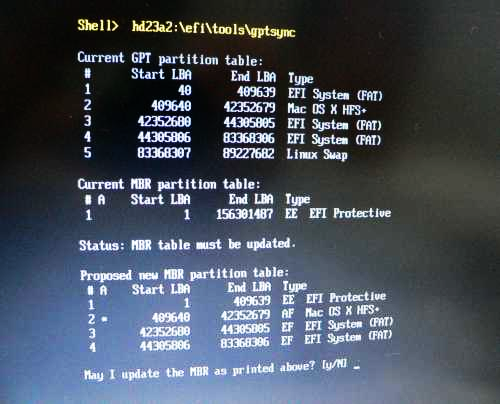
\includegraphics[width=0.9\hsize]{image200607/gptsync.png}

$B$3$N>uBV$G!"%$%s%9%H!<%i$N2hLL$K(B Alt-F1$B$GLa$j!"(BLILO $B$r(B MBR $B$G$O$J$/!"(B
Linux $BMQ$N%Q!<%F%#%7%g%s$K%$%s%9%H!<%k$7$^$9!#:F5/F0$9$k$H(BrEFIt$B$+$i(BLinux
$B$r;XDj$7$F5/F0$G$-$k$h$&$K$J$C$F$$$^$9!#(B

\subsection{$B3F<o%G%P%$%9$N@_Dj(B}
\subsubsection{X$B$N@_Dj(B}

\texttt{X} $B$O(B \texttt{i810} $B%I%i%$%P$G@_Dj$7$^$9!#(B
\texttt{915resolution} $B%Q%C%1!<%8$r%$%s%9%H!<%k$7$^$9!#(B
$B2rA|EY$O(B 1280x800 $B$G$9!#(B

\texttt{/etc/default/915resolution}$B$NNc$G$9!'(B\\
\begin{commandline}
#
# 915resolution default
#
# find free modes by  /usr/sbin/915resolution -l
# and set it to MODE
# e.g. use MODE=54 
MODE=32
#
# and set resolutions for the mode.
# e.g. use XRESO=1024 and YRESO=768
XRESO=1280
YRESO=800
#
# We can also set the pixel mode.
# e.g. use BIT=32
# Please note that this is optional,
# you can also leave this value blank.
BIT=
\end{commandline}

xorg.conf $B$NNc$G$9(B\footnote{$B%G%U%)%k%H$G30It=PNO$b$9$k$h$&$K@_Dj$7$F$"$j$^$9(B}$B!'(B

\begin{commandline}
Section "Files"
	FontPath	"/usr/share/fonts/X11/misc"
	FontPath	"/usr/X11R6/lib/X11/fonts/misc"
	FontPath	"/usr/share/fonts/X11/cyrillic"
	FontPath	"/usr/X11R6/lib/X11/fonts/cyrillic"
	FontPath	"/usr/share/fonts/X11/100dpi/:unscaled"
	FontPath	"/usr/X11R6/lib/X11/fonts/100dpi/:unscaled"
	FontPath	"/usr/share/fonts/X11/75dpi/:unscaled"
	FontPath	"/usr/X11R6/lib/X11/fonts/75dpi/:unscaled"
	FontPath	"/usr/share/fonts/X11/Type1"
	FontPath	"/usr/X11R6/lib/X11/fonts/Type1"
	FontPath	"/usr/share/fonts/X11/100dpi"
	FontPath	"/usr/X11R6/lib/X11/fonts/100dpi"
	FontPath	"/usr/share/fonts/X11/75dpi"
	FontPath	"/usr/X11R6/lib/X11/fonts/75dpi"
	# path to defoma fonts
	FontPath	"/var/lib/defoma/x-ttcidfont-conf.d/dirs/TrueType"
EndSection

Section "Module"
	Load	"i2c"
	Load	"bitmap"
	Load	"ddc"
	Load	"dri"
	Load	"extmod"
	Load	"freetype"
	Load	"glx"
	Load	"int10"
	Load	"type1"
	Load	"vbe"
EndSection


Section "InputDevice"
	Identifier	"Generic Keyboard"
	Driver		"kbd"
	Option		"CoreKeyboard"
	Option		"XkbRules"	"xorg"
	Option		"XkbModel"	"pc104"
	Option		"XkbLayout"	"us"
	Option		"XkbOptions"	"ctrl:nocaps"
EndSection

Section "InputDevice"
	Identifier	"Configured Mouse"
	Driver		"mouse"
	Option		"CorePointer"
	Option		"Device"		"/dev/input/mice"
	Option		"Protocol"		"ExplorerPS/2"
	Option		"Emulate3Buttons"	"true"
EndSection

Section "InputDevice"
	Identifier	"Synaptics Touchpad"
	Driver		"synaptics"
	Option		"SendCoreEvents"	"true"
	Option		"Device"		"/dev/psaux"
	Option		"Protocol"		"auto-dev"
	Option		"HorizScrollDelta"	"0"
EndSection


Section "Device"
	Identifier	"Generic Video Card"
	Driver		"i810"
	Screen		0
	Option "MonitorLayout" "CRT,LFP"
	BusID		"PCI:0:2:0"
EndSection

Section "Device"
	Identifier	"Device1"
	Driver		"i810"
	Screen		1
	Option "MonitorLayout" "CRT,LFP"
	BusID		"PCI:0:2:0"
EndSection

\end{commandline}
\\$BB3$/(B

\begin{commandline}



Section "Monitor"
	Identifier	"Generic Monitor"
	Option		"DPMS"
	HorizSync	28-64
	VertRefresh	43-60
EndSection


Section "Monitor"
	Identifier	"External Monitor"
	Option		"DPMS"
	HorizSync	28-64
	VertRefresh	43-60
EndSection

Section "Screen"
	Identifier	"Default Screen"
	Device		"Generic Video Card"
	Monitor		"Generic Monitor"
	DefaultDepth	24
	SubSection "Display"
		Depth		1
		Modes		"1280x800" "1024x768" "800x600" "640x480"
	EndSubSection
	SubSection "Display"
		Depth		4
		Modes		"1280x800" "1024x768" "800x600" "640x480"
	EndSubSection
	SubSection "Display"
		Depth		8
		Modes		"1280x800" "1024x768" "800x600" "640x480"
	EndSubSection
	SubSection "Display"
		Depth		15
		Modes		"1280x800" "1024x768" "800x600" "640x480"
	EndSubSection
	SubSection "Display"
		Depth		16
		Modes		"1280x800" "1024x768" "800x600" "640x480"
	EndSubSection
	SubSection "Display"
		Depth		24
		Modes		"1280x800" "1024x768" "800x600" "640x480"
	EndSubSection
EndSection

Section "Screen"
	Identifier "Secondary Screen"
	Device "Device1"
	Monitor "External Monitor"
	DefaultDepth 24
	SubSection "Display"
		   Depth 1
		   Modes "1024x768" "800x600"
	EndSubSection
	SubSection "Display"
		   Depth 4
		   Modes "1024x768" "800x600"
	EndSubSection
	SubSection "Display"
		   Depth 8
		   Modes "1024x768" "800x600"
	EndSubSection
	SubSection "Display"
		   Depth 16
		   Modes "1024x768" "800x600"
	EndSubSection
	SubSection "Display"
		   Depth 24
		   Modes "1024x768" "800x600"
	EndSubSection
EndSection

Section "ServerLayout"
	Identifier "Dual-monitor Layout"
	Screen 0 "Default Screen"
	Screen 1 "Secondary Screen" LeftOf "Default Screen"
	# Option "Clone" "On"
	#Option "Xinerama" "On"
	InputDevice "Generic Keyboard"
	InputDevice "Configured Mouse"
	InputDevice "Synaptics Touchpad"
EndSection

Section "DRI"
	Mode	0666
EndSection
 
\end{commandline}

$B%-!<%P%$%s%I$O(B .xsession \footnote{$B:G6a$O%G%U%)%k%H$G$O!!(B.gnomerc$B!!$H$$(B
$B$&%U%!%$%k$,;H$o$l$k$h$&$G$9!#(B GDM$B$+$i%G%U%)%k%H$N%7%9%F%`%;%C%7%g%s$rL@(B
$B<(E*$KA*Br$9$l$P(B .xsession$B!!$r<B9T$7$F$/$l$k$h$&$G$9!#(B}$B$NCf$G<!$N$h$&$J(B
$B@_Dj$r$7$F$$$^$9!#1&$N(Bapple$B%-!<$r2!$9$HA43Q!&H>3Q%-!<$K3d$jEv$F$i$l$F$$(B
$B$^$9!#(Boption $B$H(B apple$B!!%-!<$O$h$/2!$74V0c$($k$N$G!"N>J}$r(B Alt\_L$B$H$7$F@_(B
$BDj$7$F$$$^$9!#$^$?!"%$%8%'%/%H%-!<$H%-!<%\!<%I$N2<$NItJ,$K$"$k(BENTER$B%-!<(B
$B$r%^%&%9MQ$N%-!<$H$7$FDj5A$7$F$$$^$9!#(B\footnote{xkbset$B%Q%C%1!<%8$,I,MW(B}$B!#(B
$B$^$?!"30It%^%&%9$r(BUSB$B$G@\B3$7$?>l9g$bLdBj$J$/F0:n$7$^$9!#(B

\begin{commandline}
xmodmap -e "keycode 115 = Alt_L"
xmodmap -e "keycode 116 = Zenkaku_Hankaku" # right-apple
xmodmap -e "keycode 108 = Pointer_Button3" # KP-ENTER
xmodmap -e "keycode 204 = Pointer_Button2" # eject
xkbset m
\end{commandline}

\subsubsection{lilo$B$N@_Dj(B}

$B$$$D$b$NJJ$G(Bboot(/dev/sda3, ext2)$B$H(Broot(/dev/sda4 ext3)$B$r$o$1$F$7$^$C$F$$$k$N$G$A$g$C$H$d$d$3(B
$B$7$$Nc$G$9$,!"8=:_MxMQ$7$F$$$k(Blilo.conf $B$NNc$G$9!'(B

\begin{commandline}
boot=/dev/sda3
root=/dev/sda4
map=/boot/map
delay=20
default=Linux-20060705

image=/boot/vmlinuz-2.6.17dancer-20060701
        label=Linux-20060701
        read-only

image=/boot/vmlinuz-2.6.17dancer
        label=Linux-20060705
        read-only

image=/vmlinuz
        label=Linux
        read-only

image=/vmlinuz.old
        label=LinuxOLD
        read-only
        optional
        initrd=/initrd.img.old

\end{commandline}


$B%G%U%)%k%H$G%$%s%9%H!<%k$5$l$F$$$k%+!<%M%k$,!!(B2.6.17 $B0JA0$N$b$N$G$"$l$P!"(B
$B$h$/5/F0;~$K%Q%K%C%/$r$*$3$9$N$G!"(BIntel Mac $BBP1~$N!!(B2.6.17 $B0J9_$N$b$N$K(B
$BJQ99$7$^$7$g$&!#(B

\subsubsection{$B%5%&%s%I%+!<%I@_Dj(B}

$B%5%&%s%I%+!<%I$O!!(B\texttt{snd\_hda\_intel}$B!!%I%i%$%P$GBP1~$G$-$k(B ALSA$B$N%*!<%G%#%*%G(B
$B%P%$%9$G$9!#(B

\begin{commandline}
$ cat /proc/asound/cards
 0 [Intel          ]: HDA-Intel - HDA Intel
                      HDA Intel at 0x90440000 irq 50
\end{commandline}

\subsubsection{CPU$B$NF0E*<~GH?t@_Dj(B}

cpufreq $B$O(B \texttt{speedstep\_centrino}$B!!$GF0:n$7$^$9!#(B
apt-get install cpufreqd $B$G%$%s%9%H!<%k$7$F!"(Bcpufreqd$B!!$rF0:n$5$;$F$"$2(B
$B$k$H!"F0:n$7$^$9!#(B

\subsubsection{USB$B$N@_Dj(B}

USB$B$O!!(BUHCI, EHCI$B!!$G$9!#(B
$BDL>o$OFC$K@_DjI,MW$J$$$O$:$G$9!#(B

\subsubsection{$BEE8;@_Dj(B}

$B%P%C%F%j!<$O$^$H$b$K%5%]!<%H$7$F$$$k$h$&$G$9!#(B
$B$?$@!"EE8;$NA4MFNL$,=P$F$$$J$$$N$G!"(Bgnome$B$+$iJQ$J%a%C%;!<%8$O=P$^$7$?!#(B

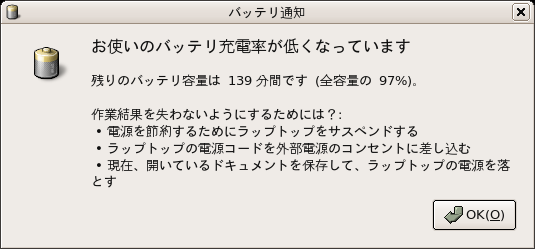
\includegraphics[width=0.8\hsize]{image200607/batterylo.png}

\subsubsection{$B%M%C%H%o!<%/$N@_Dj(B}

$BM-@~%M%C%H%o!<%/$O(B SKY2 $B$N%I%i%$%P$rMxMQ$7$^$9!#(B

$BL5@~%M%C%H%o!<%/$O!!(Bmadwifi $B$GBP1~$G$-$^$9!#(B
$B%$%s%9%H!<%kJ}K!$O2<5-$G$9!#(B

\begin{itemize}
  \item \texttt{sudo apt-get install madwifi-source madwifi-tools madwifi-doc}
  \item \texttt{sudo m-a prepare}
  \item \texttt{sudo m-a a-i madwifi}
  \item \texttt{sudo modprobe ath\_pci}
\end{itemize}

$BJ|$C$F$*$/$H(Bhotplug$B$K$h$j!"5/F0;~$K<+F0%m!<%I$5$l$FM-8z$K$J$j$^$9!#(B
\texttt{/etc/hotplug/blacklist.d/}$B$K%U%!%$%k$r:n@.$7!"2<5-$N$h$&$JFbMF$r(B
$BDI2C$7$F$*$/$H<jF0$G%m!<%I$7$J$$$HM-8z$K$J$i$J$$$h$&$K$G$-$^$9!#Ht9T5!$K(B
$B$N$k>l9g$J$I$N$?$a$K$OI,MW$+$b$7$l$^$;$s!#(B

\begin{commandline}
 ath_pci
\end{commandline}

$B0J2<!"%$%s%9%H!<%k;z$N%m%0$NNc$G$9!#(B

\begin{commandline}
 $ sudo apt-get install madwifi-source madwifi-tools madwifi-doc
 $ sudo m-a prepare
Getting source for kernel version: 2.6.17dancer
/lib/modules/2.6.17dancer/source $B$N%+!<%M%k%X%C%@$rMxMQ$G$-$^$9(B
symlink $B$r:n@.Cf(B...
apt-get install build-essential
$B%Q%C%1!<%8%j%9%H$rFI$_9~$s$G$$$^$9(B... $B40N;(B
$B0MB84X78%D%j!<$r:n@.$7$F$$$^$9(B... $B40N;(B
$B0J2<$N%Q%C%1!<%8$,?7$?$K%$%s%9%H!<%k$5$l$^$9(B:
  build-essential
$B%"%C%W%0%l!<%I(B: 0 $B8D!"?75,%$%s%9%H!<%k(B: 1 $B8D!":o=|(B: 0 $B8D!"J]N1(B: 94 $B8D!#(B
6916B $B$N%"!<%+%$%V$r<hF@$9$kI,MW$,$"$j$^$9!#(B
$BE83+8e$KDI2C$G(B 20.5kB $B$N%G%#%9%/MFNL$,>CHq$5$l$^$9!#(B
$B<hF@(B:1 http://ftp.jp.debian.org sid/main build-essential 11.2 [6916B]
6916B $B$r(B 0s $B$G<hF@$7$^$7$?(B (81.0kB/s)
$B%Q%C%1!<%8%U%#!<%k%I$rFI$_9~$s$G$$$^$9(B... $B40N;(B
$B%Q%C%1!<%8>uBV$rFI$_9~$s$G$$$^$9(B... $B40N;(B
$B%P%0%l%]!<%H$r<hF@$7$F$$$^$9(B... $B40N;(B
($B%G!<%?%Y!<%9$rFI$_9~$s$G$$$^$9(B ... $B8=:_(B 101852 $B8D$N%U%!%$%k$H%G%#%l%/%H%j$,%$%s%9%H!<%k$5$l$F$$$^$9!#(B)
(.../build-essential_11.2_i386.deb $B$+$i(B) build-essential $B$rE83+$7$F$$$^$9(B...
build-essential (11.2) $B$r@_Dj$7$F$$$^$9(B ...

$B40N;(B!
$ sudo m-a a-i madwifi
$B%Q%C%1!<%8%j%9%H$rFI$_9~$s$G$$$^$9(B... $B40N;(B
$B0MB84X78%D%j!<$r:n@.$7$F$$$^$9(B... $B40N;(B
madwifi-source $B$O$9$G$K:G?7%P!<%8%g%s$G$9!#(B
$B%"%C%W%0%l!<%I(B: 0 $B8D!"?75,%$%s%9%H!<%k(B: 0 $B8D!":o=|(B: 0 $B8D!"J]N1(B: 94 $B8D!#(B

1 $B%Q%C%1!<%8$K$D$$$F$N>pJs$r99?7$7$^$7$?(B
Extracting the package tarball, /usr/src/madwifi.tar.bz2, please wait...
\end{commandline}

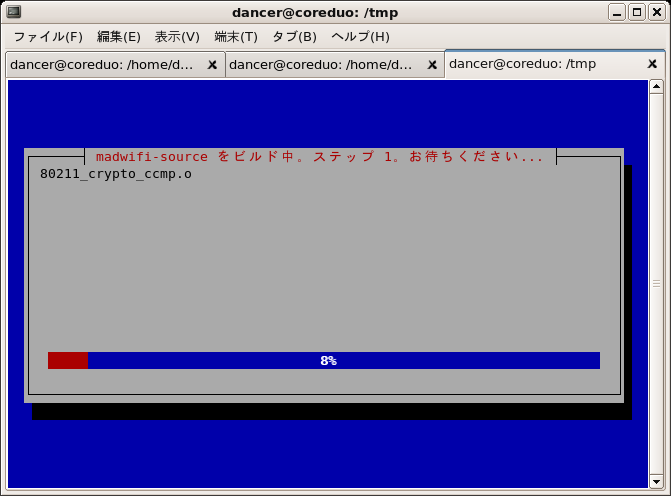
\includegraphics[width=0.8\hsize]{image200607/madwifi.png}

\begin{commandline}
/home/dancer/shared/git/madwifi-modules-2.6.17dancer_0.svnr1644.0.9.0-2+20060705_i386.deb $B$,40N;$7$^$7$?!#(B
$BL$A*Br%Q%C%1!<%8(B madwifi-modules-2.6.17dancer $B$rA*Br$7$F$$$^$9!#(B
($B%G!<%?%Y!<%9$rFI$_9~$s$G$$$^$9(B ... $B8=:_(B 101861 $B8D$N%U%!%$%k$H%G%#%l%/%H%j$,%$%s%9%H!<%k$5$l$F$$$^$9!#(B)
(.../madwifi-modules-2.6.17dancer_0.svnr1644.0.9.0-2+20060705_i386.deb $B$+$i(B) madwifi-modules-2.6.17dancer 
$B$rE83+$7$F$$$^$9(B...
madwifi-modules-2.6.17dancer (0.svnr1644.0.9.0-2+20060705) $B$r@_Dj$7$F$$$^$9(B ...

$ sudo modprobe ath_pci
$ lsmod | grep ath_pci
ath_pci                82212  0
ath_rate_sample        11776  1 ath_pci
wlan                  167132  4 wlan_scan_sta,ath_pci,ath_rate_sample
ath_hal               192208  3 ath_pci,ath_rate_sample
$ dmesg | tail -20
eth1: no IPv6 routers present
ath_hal: module license 'Proprietary' taints kernel.
ath_hal: 0.9.17.2 (AR5210, AR5211, AR5212, RF5111, RF5112, RF2413, RF5413)
wlan: 0.8.4.2 (svn r)
ath_rate_sample: 1.2 (svn r)
ath_pci: 0.9.4.5 (svn r)
Device `[PXS2]is not power manageable<6>ACPI: PCI Interrupt 0000:02:00.0[A] -> GSI 17 (level, low) -> IRQ 169
PCI: Setting latency timer of device 0000:02:00.0 to 64
wifi0: 11a rates: 6Mbps 9Mbps 12Mbps 18Mbps 24Mbps 36Mbps 48Mbps 54Mbps
wifi0: 11b rates: 1Mbps 2Mbps 5.5Mbps 11Mbps
wifi0: 11g rates: 1Mbps 2Mbps 5.5Mbps 11Mbps 6Mbps 9Mbps 12Mbps 18Mbps 24Mbps 36Mbps 48Mbps 54Mbps
wifi0: H/W encryption support: WEP AES AES_CCM TKIP
wifi0: mac 10.3 phy 6.1 radio 10.2
wifi0: Use hw queue 1 for WME_AC_BE traffic
wifi0: Use hw queue 0 for WME_AC_BK traffic
wifi0: Use hw queue 2 for WME_AC_VI traffic
wifi0: Use hw queue 3 for WME_AC_VO traffic
wifi0: Use hw queue 8 for CAB traffic
wifi0: Use hw queue 9 for beacons
wifi0: Atheros 5424: mem=0x90100000, irq=169

$ /sbin/ifconfig ath0
ath0      $B%j%s%/J}K!(B:$B%$!<%5!<%M%C%H(B  $B%O!<%I%&%'%"%"%I%l%9(B 00:16:CB:BA:76:E7 
          inet$B%"%I%l%9(B:192.168.22.42 $B%V%m!<%I%-%c%9%H(B:192.168.22.255 $B%^%9%/(B:255.255.255.0
          inet6$B%"%I%l%9(B: fe80::216:cbff:feba:76e7/64 $BHO0O(B:$B%j%s%/(B
          UP BROADCAST RUNNING MULTICAST  MTU:1500  Metric:1
          RX packets:1176 errors:0 dropped:0 overruns:0 frame:0
          TX packets:1607 errors:0 dropped:0 overruns:0 carrier:0
      $B>WFM(B(Collisions):0 TX$B%-%e!<D9(B:0 
          RX bytes:230678 (225.2 KiB)  TX bytes:1306390 (1.2 MiB)

\end{commandline}




\subsubsection{$B%j%b%3%s(B}

$B@V30@~$N%j%b%3%s$O;H$($k$h$&$G$9!#%+!<%M%kMQ$N%G%P%$%9%I%i%$%P$,B8:_$7$^(B
$B$9!#(B2.6.18$B0J9_$K$H$j$3$^$l$k$N$G$O$J$$$G$7$g$&$+!)(B
$B%f!<%66u4V$GMxMQ$G$-$k%I%i%$%P$O:n@.$7$F$*$-$^$7$?!#(B
\footnote{\url{http://www.netfort.gr.jp/~dancer/diary/daily/2006-Jul-12.html.ja}}

\subsubsection{iSight}

iSight $B$O(B linux-uvc$B%G%P%$%9$G$9!#(B
$B%U%!!<%`%&%'%"$N%m!<%I$,I,MW$G$9!#(B
$B<!$N<j=g$G%$%s%9%H!<%k$,$G$-$^$9!#(B

\begin{itemize}
 \item \texttt{apt-get install linux-uvc-tools linux-uvc-source}
 \item \texttt{module-assistant auto-install linux-uvc}
\end{itemize}

$B%"%W%j%1!<%7%g%s$O(Bekiga$B$J$I$rMxMQ$7$^$7$g$&!#(B
v4l2$B%G%P%$%9$J$N$G!"(Bv4l2$BBP1~$N%=%U%H%&%'%"$,I,MW$G$9!#(B

\begin{itemize}
 \item \texttt{apt-get install ekiga libpt-plugins-v4l2}
\end{itemize}

$B<B:]$K%m!<%I$9$k$K$O!"(BMac OS X$B$N%G%P%$%9%I%i%$%P$KF~$C$F$$$k%U%!!<%`%&%'(B
$B%"$r%m!<%I$7$F$+$i%b%8%e!<%k$r%m!<%I$7$^$9!#%I%i%$%P$N$"$k>l=j$N%G%#%l%/(B
$B%H%j3,AX$,?<$$$N$GCm0U!#(B

\begin{itemize}
 \item \texttt{sudo mount /dev/sda2 /mnt/macosx}
 \item \texttt{sudo macbook-isight-firmware-loader \\
       /mnt/mac/System/Library/Extensions/IOUSBFamily.kext/Contents/PlugIns($B<!$N9T$KB3$/(B)\\/AppleUSBVideoSupport.kext/Contents/MacOS/AppleUSBVideoSupport}
 \item \texttt{modprobe uvcvideo}
\end{itemize}


\subsubsection{$BL$3NG'$N%G%P%$%9!"<jK!(B}

Debian$B$r<+F05/F0$5$;$kJ}K!$,$o$+$j$^$;$s!"(BrEFIt$B$O%G%U%)%k%H$G$O!"(BMacOSX
$B$b$7$/$O(BeLILO$B$r5/F0$7$h$&$H$7$F$7$^$$$^$9!#(BeLILO$B$r5/F0$9$k$H5/F0$G$-$J$$!#(B
$BM%@hEY$NJQ99$O$I$&$d$C$?$i$h$$$N$+!"$H$$$&$N$,$$$^$$$AITL@$G$9!#(B

$B%5%9%Z%s%I$NJ}K!!#(B

$B%9%j!<%W$NJ}K!!#(B

CD-R$B$NF0:n$O$^$@3NG'$7$F$$$^$;$s!#(BPATA$B%Q%C%A$,I,MW$H$$$&1=$G$9!#(B

\begin{commandline}
 
 # cdrecord -scanbus
 scsibus0:
        0,0,0     0) *
        0,1,0     1) 'ATA     ' 'ST98823AS       ' '7.01' Disk
        0,2,0     2) *
        0,3,0     3) *
        0,4,0     4) *
        0,5,0     5) *
        0,6,0     6) *
        0,7,0     7) *
\end{commandline}

$B%P%C%/%i%$%H$N@)8f$,$G$-$k%I%i%$%P$O:n@.$5$l$F$$$k$N$G!"(B2.6.18$B$+(B19$B$/$i$$(B
$B$K$OF~$k$N$G$O$J$$$G$7$g$&$+!#(B

bluetooth$B$K$D$$$F$OL$D4::!#(B

\subsection{$BH/I=MzNr(B}

$BK\;qNA$O2<5-$N>l=j$G$NH/I=;qNA$H$7$F:n@.$5$l$?$b$N$G$9!#(B
$BFbMF$K$D$$$F$O?o;~99?7$7$J$,$i!"$$$/$D$+$N>l=j$GH/I=$7$F$$$^$9!#(B

\begin{itemize}
 \item 2006$BG/(B7$B7n(B2$BF|(B $B=)MU86!"(BCodeFestAkihabara  2006:$B!!:G=*Js9p(B
 \item 2006$BG/(B7$B7n(B6$BF|(B $B7CHf<w!"(BSGI$B%[!<%k!"%+!<%M%kFI=q2q(B: mixi.jp $B$NOC$NA0:B(B
 \item 2006$BG/(B7$B7n(B15$BF|(B $BKL3$F;!"(BOSC-Do 2006: $B!V(BDebian$BJY6/2q!W$N%;%C%7%g%s(B
 \item 2006$BG/(B7$B7n(B29$BF|(B $BF|!9C+!"(BTLUG: $B!V(BMacBook$B$K(BMac OS X$B$H(BDebian$B$r(B
       dual-boot$B$G%$%s%9%H!<%k!W(B
\end{itemize}

\subsection{$B;29MJ88%(B}

$B%U%!!<%`%&%'%"$N(B bootcamp$B!!$^$o$j$N3+H/$N1F6A$G!"$[$H$s$I$N(Bweb$B>e$N<j=g$r(B
$B=q$$$F$"$kJ88%$O8=:_$N;~E@$G<j=g$,8E$/$J$C$F$$$k$N$G!";29M$K$J$i$J$$>l9g(B
$B$,B?$$$G$9$,!":#8e99?7$5$l$k$+$b$7$l$^$;$s!#(B

\begin{itemize}
 \item MacBook Developer Note: MacBook$B$NO@M}9=@.?^!"%O!<%I%&%'%"$N354Q$,2r@b$5$l$F$$$^$9!#!!(B
       \url{http://developer.apple.com/documentation/HardwareDrivers/Conceptual/MacBook_0605/index.html}
 \item $B@V30@~%j%b!<%H%3%s%H%m!<%kMQ!"(BIR Receiver$B!!%Q%C%A(B
       \url{http://sourceforge.net/mailarchive/message.php?msg_id=16309282}
       \url{http://www.madingley.org/macmini/kernel/ir.patch}
 \item $B@V30@~%j%b!<%H%3%s%H%m!<%k$G(BXPDF$B%W%l%<%s%F!<%7%g%s$9$k%Q%C%A!#(B
       \url{http://www.netfort.gr.jp/~dancer/diary/daily/2006-Jul-12.html.ja#2006-Jul-12-00:00:06}
 \item MacBook $B$N;EMM!'!!4JC1$K35MW$@$1$,@bL@$5$l$F$$$^$9!#(B
       \url{http://support.apple.com/specs/macbook/macbook.html}
 \item iSight (IEEE1394 $B30It%G%P%$%9(B)$B$N%W%m%0%i%_%s%0%,%$%I!!(B
       \url{http://developer.apple.com/documentation/Hardware/Conceptual/iSightProgGuide/
iSightProgGuide.pdf}
 \item bluetooth $B$N%I%-%e%a%s%H!'!!(B\url{http://developer.apple.com/documentation/HardwareDrivers/Conceptual/HWTech_Bluetooth/index.html#//apple_ref/doc/uid/TP40003032}
 \item mactel linux$B$N%Z!<%8!!(B\url{http://mactel-linux.org/}$B!"(B
       $B$3$3$+$i$?$I$l$k%a!<%j%s%0%j%9%H$GM-MQ$J>pJs$,8r49$5$l$F$$$^$9!#(B
 \item rEFIt$B$N%Z!<%8!!(B\url{http://refit.sourceforge.net/}
 \item \url{http://sharealike.org/index.php?m=200605}
 \item $B%P%C%/%i%$%H@)8f(B
       \url{http://modular.math.washington.edu/macbook/backlight/}
 \item Ubuntu$B$N%$%s%9%H!<%k$K$D$$$F$N$^$H$a%Z!<%8(B
       \url{http://desrt.mcmaster.ca/macbook.xhtml}
 \item Gentoo $B$N>pJs%Z!<%8!!(B
       \url{http://gentoo-wiki.com/HARDWARE_Apple_MacBook}
 \item MadWifi Wiki
       \url{http://madwifi.org/wiki/UserDocs/Distro/Debian/MadWifing}
 \item Macbook Pro build-in iSight
       \url{http://blogs.gnome.org/view/rbultje/2006/07/08/0}
 \item linux usb video class, linux-uvc
       \url{http://linux-uvc.berlios.de}
 \item Debian wiki MacBook \url{http://wiki.debian.org/MacBook}
\end{itemize}

\dancersection{$B$"$J$?$,CN$i$J$$$&$A$K;H$C$F$$$k(BDebian specific}{$B_7ED$5$s(B}
\label{sec:sawadadebianspecific}

\subsection{$B$O$8$a$K(B}

Debian$B%Q%C%1!<%8$r4IM}$9$k$?$a$N%D!<%k$G$"$k(Bapt$B$d(Bdpkg$B$J$I$O0lL\$G(B
Debian specific$B$H$o$+$j$^$9!#(B
$B$7$+$7!"F|>oE*$KMxMQ$7$F$$$k%3%^%s%I!"@_Dj%U%!%$%k$J$I(B
$B$G$b<B$O(BDebian$B8GM-$N$b$N$G$"$C$?$j(B
$B%Q%C%1!<%82=$9$k:]$KJQ99$,2C$($i$l$F$$$?$j$9$k$b$N$,$"$j$^$9!#(B
$B$3$3$G$O$=$N$h$&$J$"$J$?$NCN$i$J$$(BDebian specific$B$r>R2p$7$^$9!#(B

\subsection{adduser}

Debian$B$G(B

\begin{commandline}
# adduser hoge
\end{commandline}

$B$r<B9T$9$k$H(Bhoge$B%f!<%6$,:n$i$l%Q%9%o!<%I$NF~NO$,5a$a$i$l$^$9!#(B
Fedora$B$GF1$8%3%^%s%I%i%$%s$r<B9T$7$?>l9g!"(Bhoge$B%f!<%6$O:n$i$l$^$9$,(B
$B%Q%9%o!<%IF~NO$O5a$a$i$l$^$;$s!#%Q%9%o!<%I$OJLES(Bpasswd$B%3%^%s%I$G@_Dj$9$k(B
$BI,MW$,$"$j$^$9!#(B

$B$3$N0c$$$O(BDebian$B$N(Badduser$B$H(BFedora$B$G(Badduser$B$N<BBN$N0c$$$K$h$k$b$N$G$9!#(B
Fedora$B$N(Badduser$B$O(Buseradd$B$X$N%7%s%\%j%C%/%j%s%/$G$9!#(B
Debian$B$N(Badduser$B$O(BPerl$B%9%/%j%W%H$G!"(Buseradd$B!"(Bpasswd$BEy$r(B
$B8F$S=P$7$F%f!<%6$r:n@.$7$F$$$^$9(B\footnote{$B%Q%9%o!<%IF~NO$N%W%m%s%W%H$O(B
passwd$B%3%^%s%I$,I=<($7$F$$$^$9(B}$B!#(B

$B$A$J$_$K!"(BFreeBSD$B$N(Badduser$B$O%7%'%k%9%/%j%W%H$G=q$+$l$F$*$j!"(Bpw$B$H$$$&%3%^(B
$B%s%I$r8F$S=P$9$3$H$G%f!<%6$NDI2C$r9T$C$F$$$k$h$&$G$9!#(B
Debian GNU/kFreeBSD$B$O(BFreeBSD$B%+!<%M%k$N>e$K(BGNU$B$N%D!<%k$d(Bglibc$B!"(BDebian$B$N%D!<(B
$B%k$r>h$;$?$b$N$G$"$k$?$a!"(BDebian$B$N(Badduser$B$,;H$o$l$F$*$j!"(Buseradd$B$H(Bpasswd
$B$G%f!<%6$NDI2C$r9T$C$F$$$^$7$?!#(B

\subsection{ifup}

$B%M%C%H%o!<%/$N@_Dj$rJQ$($?$N$G%$%s%?!<%U%'!<%9$r:F5/F0$7$?$$$H$$$&>l9g!"(B
Debian$B$G$O0J2<$N%3%^%s%I%i%$%s$r<B9T$9$k$H(Bauto$B$K@_Dj$5$l$F$$$k(B
$B%$%s%?!<%U%'!<%9$r$9$Y$F:F5/F0$9$k$3$H$,$G$-$^$9!#(B

\begin{commandline}
# ifdown -a \&\& ifup -a
\end{commandline}

$B0lJ}(BFedora$B$G$O(B-a$B%*%W%7%g%s$O;H$($:!"$^$?!"J#?t$N%$%s%?!<%U%'!<%9$r;XDj$9(B
$B$k$3$H$O$G$-$^$;$s!#(B

$B%$%s%?!<%U%'!<%9$N@_Dj%U%!%$%k$b(BDebian$B$G$O(B/etc/network/iterfaces$B!"(B
Fedora$B$G$O(B/etc/sysconfig/network-scripts/ifcfg-$<$$B%$%s%?!<%U%'!<%9L>(B$>$
$B$H$J$C$F$*$j!"%U%)!<%^%C%H$O$^$C$?$/0c$$$^$9!#(B

\subsection{Xsession}

startx$B$N(Bman$B$r8+$k$H(BX$B$N5/F0;~$K<B9T$5$l$k%9%/%j%W%H$O(B~/.xinitrc$B$H$J$C$F(B
$B$$$^$9!#$7$+$7!"(BDebian$B$G$O(B~/.xsession$B$K=q$$$F$*$1$P(Bstartx$B$r<B9T$7$?$H(B
$B$-$G$b%0%i%U%#%+%k%m%0%$%s$7$?$H$-$G$bF1$84D6-$K$9$k$3$H$,$G$-$^$9!#(B

$B$3$l$O!"(BDebian$B$G$OAG$N(BX$B$KBP$7$FJQ99$r2C$($F$$$k$?$a$G$9!#(B

startx$B$7$?$H$-$N%U%m!<$O<!$N$h$&$K$J$C$F$$$^$9!#(B
\begin{enumerate}
\item /usr/bin/startx
\item ~/.xinitrc$B$,$"$C$?$i(B~/.xinitrc$B$r<B9T!#$J$+$C$?$i(B
	  /etc/X11/xinit/xinitrc(Debian$B8~$1$K=$@5$5$l$F$$$^$9(B)$B$r<B9T(B
\item /etc/X11/Xsession$B$r<B9T(B
\end{enumerate}

$B%0%i%U%#%+%k%m%0%$%s(B(xdm)$B$7$?>l9g$N%U%m!<$O<!$N$h$&$K$J$j$^$9!#(B
\begin{enumerate}
\item /etc/X11/xdm/xdm-config$B$N(BDisplayManager*session$B$K=q$+$l$?%3%^%s%I(B
	  ($BDL>o!"(B/etc/X11/xdm/Xsession(Debian$B8~$1$K=$@5$5$l$F$$$^$9(B))$B$r<B9T(B
\item /etc/X11/Xsession$B$r<B9T(B
\end{enumerate}

$B$H$$$&$o$1$G$I$A$i$N>l9g$b(B/etc/X11/Xsession$B$,<B9T$5$l$^$9!#(B
$B$3$N(B/etc/X11/Xsession$B$O(BDebian specific$B$J$b$N$G(B/etc/X11/Xsession.d$B%G%#%l(B
$B%/%H%j$K$"$k%9%/%j%W%H$r=g$K<B9T$7$^$9!#(B
$B$3$N$&$A!"(B50x11-common\_determine-startup$B$G5/F0%W%m%0%i%`$N8!=P$,9T$o$l!"(B
~/.xsession$B$,$"$k>l9g!"(B~/.xsession$B$,5/F0%W%m%0%i%`$KA*$P$l$^$9!#(B
99x11-common\_start$B$G(B50x11-common\_determine-startup$B$GA*$P$l$?%W%m%0%i%`(B
$B$,<B9T$5$l$k$3$H$G(B~/.xsession$B$K=q$+$l$?FbMF$,M-8z$K$J$j$^$9!#(B

$B$A$J$_$K!"(BFedora$B$G$O(B~/.Xclients$B$K=q$/$H(Bstartx$B$G$b%0%i%U%#%+%k%m%0%$%s$G(B
$B$b%9%/%j%W%H$r<B9T$7$F$/$l$k$h$&$G$9!#$?$@$7!"(B/etc/X11/Xsession.d$B%G%#%l(B
$B%/%H%j$N$h$&$J;EAH$_$O$J$$$h$&$G$9!#(B

\subsection{lesspipe}

less$B$G(Bgzip$B05=L$5$l$?%U%!%$%k$r3+$3$&$H$9$k$HDL>o<!$N$h$&$K$J$j$^$9!#(B

\begin{commandline}
$ less hoge.txt.gz
"hoge.txt.gz" may be a binary file.  See it anyway?
\end{commandline}

$B$R$g$C$H$7$?$i>e$N$h$&$J%a%C%;!<%8$OI=<($5$l$:$K(B
hoge.txt$B$NFbMF$,I=<($5$l$F$$$kJ}$b$$$i$C$7$c$k$+$b$7$l$^$;$s!#(B
$B$=$N>l9g!"<!$N4D6-JQ?t$,@_Dj$5$l$F$$$k$O$:$G$9!#(B

\begin{commandline}
$ printenv | grep ^LESS
LESS=-M
LESSOPEN=| /usr/bin/lesspipe '%s'
LESSCLOSE=/usr/bin/lesspipe '%s' '%s'
\end{commandline}

less$B$K$O(BLESSOPEN$B$H$$$&4D6-JQ?t$,@_Dj$5$l$F$$$k$H%U%!%$%k$rFI$_9~$`A0(B
$B$K(BLESSOPEN$B$G;XDj$5$l$?%3%^%s%I$K%U%!%$%kL>$rEO$7$F%3%^%s%I$NI8=`=PNO$r%U%!(B
$B%$%k$NFbMF$H$7$FFI$_9~$`$H$$$&5!G=$,$"$j$^$9!#(B
$B$3$l$K$h$j!"(Bgzip$B05=L$5$l$?%U%!%$%k$r(B

\begin{commandline}
$ less hoge.txt.gz
\end{commandline}

$B$H$$$&%3%^%s%I%i%$%s$GI=<($9$k$3$H$,$G$-$^$9!#(B
$B$^$?!"$3$N5!G=$r1~MQ$9$k$3$H$G(B

\begin{commandline}
$ less hoge.tar.gz
\end{commandline}

$B$H$7$?>l9g$K(Btar$B$5$l$F$$$k%U%!%$%k$N0lMw$r<hF@$9$k$H$$$C$?$3$H$b$G$-$^$9!#(B

/usr/bin/lesspipe$B$O(BDebian specific$B$J$b$N$G$9!#B>$N%G%#%9%H%j%S%e!<%7%g%s(B
$B$K$bF1MM$N5!G=$r;}$D$b$N$,4^$^$l$F$$$k$3$H$,B?$$$N$G$9$,!"(BDebian$B$N(B
lesspipe$B$OBP1~$7$F$$$k3HD%;R$N?t$,B?$$$3$H$,FCD'$G$9!#(B

language-env$B$r<B9T$9$k$H(BLESSOPEN$B$N@_Dj$r$7$F$/$l$k$?$a(B
$B5$$E$+$:;H$C$F$$$k$H$$$&J}$b$$$i$C$7$c$k$N$G$O$J$$$G$7$g$&$+!#(B

\subsection{Debian specific$B$N8+$D$1J}(B}

$B$=$l$,(BDebian specific$B$G$"$k$+CN$k$?$a$K$O(Bman$B$r;2>H$9$k$H$$$&J}K!$,$"$j$^(B
$B$9!#(Bman$B$r8+$k$H!"(B

\begin{commandline}
Debian GNU/Linux        Version 3.97        ADDUSER(8)
\end{commandline}

$B$N$h$&$K=q$+$l$F$$$k$N$G(BDebian specific$B$H?dB,$9$k$3$H$,$G$-$^$9!#(B
$B$7$+$7!"$=$l0J30$K(BDebian specific$B$+$rCN$k$h$$J}K!$O$J$$$h$&$G$9!#(B

Xsession$B$d(Blesspipe$B$N$h$&$K%*%j%8%J%k$NG[I[FbMF$+$i%U%!%$%k$,DI2C$5$l$F$$(B
$B$k>l9g!"%=!<%9%Q%C%1!<%8$N(Bdebian$B%G%#%l%/%H%j$KDI2C%U%!%$%k$,3JG<$5$l$F$$(B
$B$^$9!#(B
debian$B%G%#%l%/%H%j$K$"$k%U%!%$%k%j%9%H$+$i(Bcontrol$B$d(Bpostinst$B$J$I$N@)8f%U%!(B
$B%$%k$r=|$$$?$b$N$r<hF@$9$l$P$=$N%Q%C%1!<%8$K(BDebian specific$B$JJQ99$,$"$j(B
$B$=$&$+?dB,$9$k$3$H$,$G$-$k$H9M$($i$l$^$9!#(B

%% $B$5$o$@$5$s$3$3$^$G(B
%% $B>.NS$5$s$3$3$+$i(B
\dancersection{$BK]Lu$X$N$5$=$$(B}{$B>.NS$5$s(B}
\label{sec:honnyaku}

\subsection{$B$O$8$a$K(B}

$B9q:]2=$O(BDebian$B$N0l$D$NFCD'$G$9!#(B
$B$=$N9q:]2=$NC#@.$K$O!"(B
$B%U%l!<%`%o!<%/$N@0Hw$+$i3F%=%U%H%&%'%"$NBP1~!"(B
$B$=$7$F%a%C%;!<%8$d%I%-%e%a%s%H$NK]Lu$^$G!"(B
$BB?4t$KEO$kHs>o$KKDBg$J:n6H$rI,MW$H$7$^$9!#(B
$B$3$3$G$O!"$=$l$i$N:n6H$N$&$A!"(B
$B:G$bBgNL$N:n6H$rI,MW$H$9$k0lJ}$G0lHL%f!<%6$,:G$b<h$jAH$_$d$9$$K]Lu$K(B
$B$D$$$F!"(B
$B<g$K(BDebian JP$B$^$o$j$G9T$o$l$F$$$kF|K\8lLu:n6H$r$^$H$a$^$9!#(B

\subsection{$B6&DL$N:n6HMQ%$%s%U%i%9%H%i%/%A%c(B}

$B$^$:!"(B
$BK]Lu:n6H$G6&DL$K;H$o$l$k%$%s%U%i%9%H%i%/%A%c$r$^$H$a$F@bL@$7$^$9!#(B
$B$3$l$i$O!"8e=R$9$k3F<o:n6H$N@bL@$G$bIQHK$KEP>l$7$^$9!#(B

\subsubsection{$B:n6HMQ%a!<%j%s%0%j%9%H(B}

$BK]Lu:n6H$K4X$9$k$d$j$H$j$K$O<g$K%a!<%j%s%0%j%9%H$,;H$o$l$^$9!#(B
Debian$BK\2H$N$b$N$H(BDebian JP$B$N$b$N$,$"$j$^$9$,!"$I$A$i$K$D$$$F$b!"(B
$BK]Lu4XO"$N%a!<%j%s%0%j%9%H$OC/$G$b(B (Debian$B$*$h$S(BDebian JP$B$N%a%s%P!<$G(B
$B$J$/$F$b(B) $B<+M3$K;22C$G$-$^$9!#(B

$BF|K\8lLu4XO"$N:n6H$K4X$9$k$d$j$H$j$K$h$/;H$o$l$k$N$O!"(B
Debian JP$B$N(Bdebian-doc\footnote{\texttt{debian-doc@debian.or.jp}}$B$*$h$S(B
debian-www\footnote{\texttt{debian-www@debian.or.jp}}$B%a!<%j%s%0%j%9%H$G$9!#(B
$BEPO?$K;H$&%"%I%l%9$O!"(B
$B$=$l$>$l(B\texttt{debian-doc-ctl@debian.or.jp}$B$H(B
\texttt{debian-www-ctl@debian.or.jp}$B$G$9!#(B
$B$3$l$i$N%a!<%j%s%0%j%9%H$K4X$9$k>pJs$,!"(B
\url{http://www.debian.or.jp/MailingList.html}\footnote{%
$B=`HwCf$N?7%5%$%H$G$O(B
\url{http://www-internal.debian.or.jp/community/ml/}$B!#(B}$B$K$"$k$N$G!"(B
$B;2>H$7$F$/$@$5$$!#(B
$B2a5n$K$3$l$i$N%a!<%j%s%0%j%9%H$KEj9F$5$l$?%a!<%k$N%"!<%+%$%V$O!"(B
\url{http://lists.debian.or.jp/debian-doc/}$B$*$h$S(B
\url{http://lists.debian.or.jp/debian-www/}$B$G40A4$K8x3+$5$l$F$$$^$9!#(B

$B$5$i$K!"%Q%C%1!<%8$N99?7$KH<$&(Bdebconf-po$B$NK]Lu99?7$N0MMj$J$I!"(B
Debian$BK\2H$N3+H/<T$H$N1Q8l$G$N$d$j$H$j$K$O!"(B
$B<g$K(BDebian$BK\2H$N(Bdebian-japanese$B%a!<%j%s%0%j%9%H(B\footnote{%
\texttt{debian-japanese@lists.debian.org}}$B$,;H$o$l$^$9!#(B
$BEPO?$*$h$S%"!<%+%$%V$O(B\url{http://lists.debian.org/debian-japanese/}$B$G(B
$BMxMQ2DG=$G$9!#(B
$B%a!<%j%s%0%j%9%H$r7PM3$;$:$K!"A0$N%P!<%8%g%s$NK]Lu<T$d!"(B
$BK]Lu<T$H$7$F3hH/$K3hF0$5$l$F$$$k$+$?!"(B
$B$"$k$$$OK\2H$G3hF0$7$F$$$kF|K\?M3+H/<T$N$H$3$m$KD>@\%a!<%k$,9T$C$?$j$9$k(B
$B$3$H$b$"$j$^$9!#(B

$B$^$?!"(B
$B%I%-%e%a%s%H$NK]Lu$J$i(BDebian$BK\2H$N(Bdebian-doc$B%a!<%j%s%0%j%9%H(B\footnote{%
\texttt{debian-doc@lists.debian.org}}$B$K!"(B
$B%&%'%V%Z!<%8$NK]Lu$J$i(BDebian$BK\2H$N(Bdebian-www$B%a!<%j%s%0%j%9%H(B\footnote{%
\texttt{debian-www@lists.debian.org}}$B$K$=$l$>$lEPO?$7$F$*$/$H!"(B
$BFbMF$K4X$9$k<ALd$d4V0c$$$N=$@5$J$I$K4X$9$k$d$j$H$j$rK\2H$NJ}!9$H$G$-$^$9!#(B
$B$=$l$>$l(B\url{http://lists.debian.org/debian-doc/}$B$*$h$S(B
\url{http://lists.debian.org/debian-www/}$B$G!"(B
$BEPO?$d%"!<%+%$%V1\Mw$,$G$-$^$9!#(B

\subsubsection{$BBPLuI=(B}

$BF|K\8lLu$NBPLuI=$O!"(BDebian JP debian-doc$B%a!<%j%s%0%j%9%H$G$?$^$K(B
$BOCBj$K$J$j$^$9$,!"$J$+$J$+@0Hw$^$G$$$+$J$$$N$,8=>u$G$9!#(B
$B%a!<%j%s%0%j%9%H$GLu8l$K4X$9$kLd$$9g$o$;$r$7$?$j!"(B
$B::FI0MMj$r=P$7$F%3%a%s%H$r$b$i$C$?$j$G$-$k$N$G!"(B
$B$=$3$^$G5$$K$J$k$3$H$O$J$$$G$7$g$&!#(B
$B0l1~!"4{B8$N$$$/$D$+$NBPLuI=$r%]%$%s%?$H$7$F<($7$F$*$-$^$9!#(B
\begin{itemize}
 \item Debian JP$B$N!XN,8l$N2r@b!Y(B:
       \url{http://www.debian.or.jp/devel/abbreviation.html}
 \item Debian JP$BBPLuI=(B
       \begin{itemize}
	\item $B%=!<%9(B: \url{http://www.debian.or.jp/Documents/trans_table/}
	\item HTML$B$G$N=PNO(B:
	      \url{http://www.debian.or.jp/Documents/trans_table/trans_table.html}
	\item dict$B7A<0$G$N=PNO(B:
	      \url{http://www.debian.or.jp/Documents/trans_table/trans_table.dict}
       \end{itemize}
 \item APT, dpkg$B4XO"$NI=5-$K4X$9$kMQ8l=8(B ($BIpF#7r;V$5$s$N(BWiki):
       \url{http://kmuto.jp/open.cgi?DebianGlossary}
 \item $B$+$M$3$5$s$K$h$k!X(BSecurity$B4XO"MQ8lBPLu=8!Y(B:
       \url{http://lists.debian.or.jp/debian-www/200607/msg00120.html}
 \item $B>.NS$K$h$k(BDebian Weekly News$B4XO"$N(Bja.po\footnote{Debian Weekly
       News$BMQ(Bwml$B%U%!%$%k$N8eH>$N(BSecurity Updates$B$*$h$S(BRemoved Packages$B$+$i(B
       $BMQ8l$rCj=P$7$F(Bpo$B$H$7$?$b$N$G$9!#(B}:
       \url{http://dolphin.c.u-tokyo.ac.jp/~nori1/dwn/ja.po}
\end{itemize}

$BBPLuI=$H$$$&$o$1$G$O$"$j$^$;$s$,!"(B
$B$3$l$i$NB>$K>.NS$,Lu8l$NA*Br$K$h$/MxMQ$9$k$N$O!"(BGoogle$B$G$9!#(B
Debian$B$N%&%'%V%5%$%HA4HL$+$iLu8l$rC5$7$?$1$l$P!V(Bsite:www.debian.org$B!W$r!"(B
Debian Weekly News$B$+$iC5$7$?$1$l$P!V(Bsite:www.debian.org/News/weekly$B!W$r(B
$B$D$1$F8!:w$7!"0z$C3]$+$C$?%Z!<%8$r8+$J$,$iLu8l$r7h$a$k$H$$$&$3$H$r$h$/(B
$B$d$C$F$$$^$9!#(B

\subsection{$B3F<o%=%U%H%&%'%"$N(Bpo$B$dIUB0%I%-%e%a%s%H$NK]Lu(B}

\subsubsection{$B:n6HJ}K!(B}

$B3F<o%=%U%H%&%'%"$N%a%C%;!<%8%+%?%m%0(B (po) $B$dIUB0%I%-%e%a%s%H!"(B
manpage$B$J$I$NK]Lu$K4X$9$k5DO@$O!"(B
Debian JP$B$N(Bdebian-doc$B%a!<%j%s%0%j%9%H$G9T$o$l$F$$$^$9!#(B
$B$3$l$i$NK]Lu$O%=%U%H%&%'%"$N99?7$KH<$C$F99?7:n6H$r$9$kI,MW$,$"$k$N$G!"(B
$B<g$K3+H/85(B (upstream) $B$N%=%U%H%&%'%":n<T$J$I$H(B ($B<g$K1Q8l$G(B) $B$d$j$H$j$r(B
$B$7$J$,$i:n6H$9$k$3$H$K$J$j$^$9!#(B
$B$7$+$7!"FC$K(BDebian$B$HL)@\$K4XO"$7$?%=%U%H%&%'%"$K$D$$$F$OLu8l$,E}0l$5$l$F(B
$B$$$k$[$&$,$h$$$N$G!"(B
$BLu8lA*Br$J$I$K$D$$$F(Bdebian-doc$B%a!<%j%s%0%j%9%H$G::FI$r0MMj$9$k$3$H$,(B
$B?d>)$5$l$F$$$^$9!#(B

\subsubsection{$BK]Lu>u67$N3NG'(B}

po$B$K$D$$$F$O!"K]Lu>u67$K4X$9$k>pJs$,0J2<$N%Z!<%8$GF@$i$l$^$9!#(B
\begin{itemize}
 \item po$B%U%!%$%kK]Lu$N%Z!<%8(B (%
       \url{http://www.debian.org/international/l10n/po/})
       \begin{itemize}
	\item $BF|K\8l$NK]Lu>u67(B:
	      \url{http://www.debian.org/international/l10n/po/ja}
	\item $B8@8l$4$H$NK]Lu%i%s%-%s%0(B:
	      \url{http://www.debian.org/international/l10n/po/rank}
       \end{itemize}
 \item Debian-Installer$B$N3F8@8lK]Lu>u67(B
       \begin{itemize}
	\item $BIT0BDjHG(B (unstable):\\
	      \url{http://d-i.alioth.debian.org/l10n-stats/translation-status.html}
	\item $B%F%9%HHG(B (testing):\\
	      \url{http://d-i.alioth.debian.org/l10n-stats/translation-status-testing.html}
       \end{itemize}
\end{itemize}

\subsection{debconf-po$B4XO"(B}

\subsubsection{debconf-po$B$H$O(B}

debconf-po$B$H$O!"(B
Debian$B%Q%C%1!<%8$r%$%s%9%H!<%k$9$k:]$K$J$5$l$k@_Dj4XO"$N<ALd(B (debconf$B$N(B
$B<ALd(B) $B$KK]Lu$rDs6!$7!"(B
localize$B$5$l$?%$%s%?%U%'!<%9$G%f!<%6$,<ALd$KEz$($i$l$k$h$&$K$9$k$?$a$N(B
po$B%U%!%$%k$G$9!#(B

$BNc$($P!"(Bsarge$B$G(B\texttt{locales}$B%Q%C%1!<%8$r@_Dj$9$k>l9g!"(B
$B1Q8l$N%m%1!<%k$G$O<!$N$h$&$J2hLL$,8=$l$^$9!#(B\\
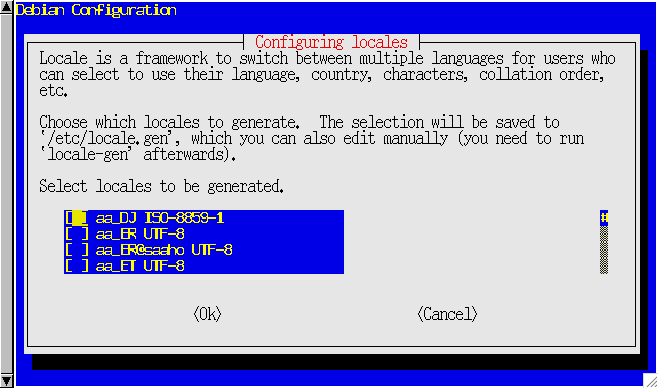
\includegraphics[width=1\hsize]{image200609/debconf-en.png}\\
$B$3$l$KBP$7$FF|K\8l$N%m%1!<%k$G$O<!$N$h$&$K$J$j$^$9!#(B\\
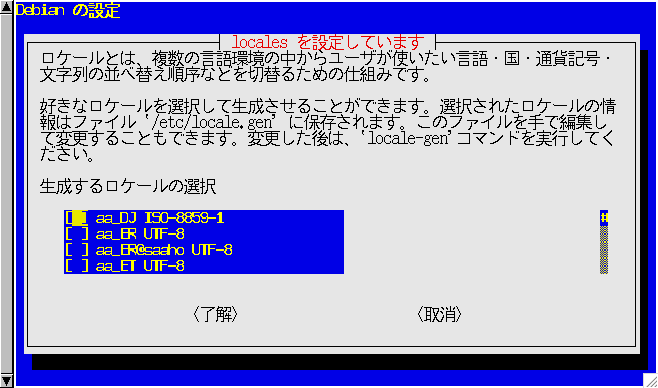
\includegraphics[width=1\hsize]{image200609/debconf-ja.png}\\
$B$3$N$h$&$K%m%1!<%k$K1~$8$?<ALd$rDs6!$9$k$N$,(Bdebconf-po$B$G$9!#(B

$B$3$N(Bdebconf$B$N<ALd<+BN$O!"<!$N$h$&$K!"%Q%C%1!<%8:n<T$K$h$C$F!"(B
$B%=!<%9%Q%C%1!<%8$N(Bdebian$B%G%#%l%/%H%j$N2<$N(B
$B%P%$%J%j%Q%C%1!<%8MQ(Btemplates$B%U%!%$%k$K1Q8l$G=q$+$l$F$$$^$9!#(B\\
\begin{commandline}
Template: locales/locales_to_be_generated
Type: multiselect
Choices: ${locales}
_Description: Select locales to be generated.
 Locale is a framework to switch between multiple languages for users who can
 select to use their language, country, characters, collation order, etc.
 .
 Choose which locales to generate.  The selection will be saved to
 `/etc/locale.gen', which you can also edit manually (you need to run
 `locale-gen' afterwards).

Template: locales/default_environment_locale
Type: select
_Choices: None, ${locales}
Default: None
_Description: Which locale should be the default in the system environment?
 Many packages in Debian use locales to display text in the correct
 language for users. You can change the default locale if you're not
 a native English speaker.
 These choices are based on which locales you have chosen to generate.
 .
 Note: This will select the language for your whole system. If you're
 running a multi-user system where not all of your users speak the language
 of your choice, then they will run into difficulties and you might want
 not to set a default locale.

\end{commandline}

$B%*%j%8%J%k$O1Q8l$G$9$,!"Hs1Q8l7w$N%f!<%6$K$H$C$F$O!"(B
$B<+J,$NJl8l$G<ALd$5$l$k$[$&$,$h$$$G$7$g$&!#(B
$B$=$3$G!"(Blocalize$B$5$l$?(Bdebconf$B<ALd$r%f!<%6$,MxMQ$G$-$k$h$&$K$9$k$N$,!"(B
$B$3$N(Bdebconf-po$B$G$9!#(B

\subsubsection{$B:n6HJ}K!(B}

$B:n6H$r3+;O$9$kA0$K!"(B
$B$^$:$O(B\ref{subsubsec:debconf-po-check}$B$G=R$Y$kK]Lu>u67D4@0%Z!<%8$G(B
$B4{$KK]Lu:n6H$,9T$o$l$F$$$J$$$+3NG'$9$k$H$h$$$G$7$g$&!#(B
$B$=$N>e$GK]LuBP>]$H$9$k%Q%C%1!<%8$r7h$a$?$i!"(B
\url{http://www.debian.org/intl/l10n/po-debconf/pot}$B$+$i$=$N%U%!%$%k$N(B
templates.pot$B%U%!%$%k$r%@%&%s%m!<%I$7$^$9!#(B
$B$b$A$m$s!"%=!<%9%Q%C%1!<%8$r<j$KF~$l!"(B
$BL\E*$N%P%$%J%j%Q%C%1!<%8$N(Btemplates$B%U%!%$%k$KBP$7$F(B
\texttt{po-debconf}$B%Q%C%1!<%8$N(B\texttt{debconf-gettextize}$B%3%^%s%I$r(B
$B<B9T$7!"(Btemplates.pot$B$r@8@.$7$F$b$+$^$$$^$;$s!#(B

templates.pot$B%U%!%$%k$r<hF@$7$?$i!"(B
$BL>A0$r(Bja.po$B$KJQ99$7$?>e$GK]Lu$7$^$7$g$&!#(B

$BK]Lu$r=*$($?$i3:Ev%Q%C%1!<%8$K(Bseverity$B$r!V(Bwishlist$B!W!"(Btags$B$r!V(Bl10n,
patch$B!W$H$7$F%P%0Js9p$7$^$7$g$&!#(B
$B$?$@!"47$l$F$$$J$$$&$A$O(BDebian JP$B$N(Bdebian-doc$B%a!<%j%s%0%j%9%H$G(B
$B::FI$7$F$b$i$&$3$H$r6/$/$*4+$a$7$^$9!#(B

% FIXME: $BM>M5$,$"$C$?$i$b$C$H=q$/(B!!

\subsubsection{$BK]Lu>u67$N3NG'(B}
\label{subsubsec:debconf-po-check}

debconf-po$B$K$D$$$F$O!"K]Lu>u67$K4X$9$k>pJs$,0J2<$N%Z!<%8$GF@$i$l$^$9!#(B
\begin{itemize}
 \item debconf-po$B%U%!%$%kK]Lu$N%Z!<%8(B (%
       \url{http://www.debian.org/international/l10n/po-debconf/})
       \begin{itemize}
	\item $BF|K\8l$NK]Lu>u67(B:
	      \url{http://www.debian.org/international/l10n/po-debconf/ja}
	\item $B8@8l$4$H$NK]Lu%i%s%-%s%0(B:
	      \url{http://www.debian.org/international/l10n/po-debconf/rank}
       \end{itemize}
 \item $BIpF#7r;V$5$s$,Ds6!$9$k(Bdebconf-po$BF|K\8lK]Lu:n6HD4@0%Z!<%8(B (%
	    \url{http://kmuto.jp/debian/po-trans/})
       $B3F%Q%C%1!<%8$N(Bdebconf-po$B$NK]Lu>u67$*$h$S:G=*Lu<T$N>pJs$r(B
       $BF@$k$3$H$,$G$-$^$9!#(B
\end{itemize}

\subsection{$B%&%'%V%Z!<%84XO"(B}

\subsubsection{Debian$B%&%'%V%Z!<%8$N;EAH$_(B}

Debian$B$N%&%'%V%Z!<%8$O(BWML$B$H$$$&%U%!%$%k7A<0$rMxMQ$7$F$$$^$9!#(B
WML$B$H$O%&%'%V%5%$%H%a%?8@8l(B (web site meta language) $B$N$3$H$G!"(B
Debian$B$G$O(B\texttt{wml}$B%Q%C%1!<%8$H$7$FDs6!$5$l$F$$$^$9!#(B
$B$3$3$G$O>\$7$/$O=R$Y$^$;$s$,!"(B
$BK]Lu$,86J8$KDI=>$G$-$F$$$k$+$N3NG'$J$I$,$3$N(BWML$B$N5!9=$rMQ$$$F(B
$B9T$o$l$F$$$k!"$H$$$&$3$H$@$1=q$$$F$*$-$^$9!#(B

$B<!$NNc$O!"(B
\url{http://www.debian.org/News/weekly/2006/35/index}$B$N%=!<%9$H$J$C$F$$(B
$B$k!"(B\texttt{cvs.debian.org}$B$N(B\texttt{webwml}$B%b%8%e!<%k(B\footnote{%
\url{http://cvs.debian.org/?root=webwml}}$B$N!"(B
\texttt{webwml/japanese/News/weekly/2006/35/index.wml}$B$G$9!#(B\\
\begin{commandline}
#use wml::debian::weeklynews::header PUBDATE="2006-08-29"
 #SUMMARY="Firmware, FrOSCon, Events, Cuba, Translations, GIT, Sarge,
 #Etch" 
#use wml::debian::translation-check translation="1.8"

<p>Welcome to this year's 35th issue of DWN, the weekly newsletter for the
Debian community.  Bug squashing parties have been announced for September 8th
to 10th in <a
href="http://lists.debian.org/debian-devel-announce/2006/08/msg00012.html">\
Vienna</a> and for September 15th to 17th in <a
href="http://lists.debian.org/debian-devel-announce/2006/08/msg00013.html">\
J&uuml;lich</a>, Germany.  OSDir has taken <a
href="http://shots.osdir.com/slideshows/slideshow.php?release=724&amp;slide=2">\
Debian installer</a>.  Petr Stehlik <a
href="http://lists.debian.org/debian-68k/2006/08/msg00234.html">reported</a>
that the installation of <a href="$(HOME)/releases/sarge/">sarge</a> and <a
href="$(HOME)/releases/etch/">etch</a> worked flawlessly in the recently <a
href="http://lists.debian.org/debian-68k/2006/08/msg00226.html">fixed</a>
version of <a href="http://packages.debian.org/aranym">ARAnyM</a>, a 32bit
Atari ST/TT/Falcon virtual machine.</p>

[snip]

#use wml::debian::weeklynews::footer editor="Sebastian Feltel, Mohammed
 Adn&egrave;ne Trojette, Tobias Toedter, Martin 'Joey' Schulze" 
\end{commandline}

$B$3$N$&$A(B\verb|#|$B$G;O$^$k9T$,(BWML$B$NL?Na$G$9!#(B
$BNc$($P!"(B\\
\begin{commandline}
#use wml::debian::translation-check translation="1.8"
\end{commandline}

$B$H$$$&9T$O!"86J8(B (\texttt{webwml/english/News/weekly/2006/35/index.wml})
$B$N(Br1.8$B$K4p$E$$$F$$$k$H$$$&0UL#$G$9!#(B

\subsubsection{$B:n6HJ}K!(B}

$BK]Lu:n6H$r3+;O$9$k$K$O!"L\E*$N%Z!<%8$N(BWML$B%U%!%$%k$rF~<j$9$kI,MW$,$"$j$^$9!#(B
CVS$B$r;H$$47$l$F$$$k>l9g$O!"(B
$B%3%^%s%I%i%$%s$+$iF|K\8l$N%D%j!<(B (\texttt{webwml/japanese}) $B$H(B
$B1Q8l$N%D%j!<(B (\texttt{webwml/english}) $B$r%A%'%C%/%"%&%H$9$k$H(B
$B$h$$$G$7$g$&!#(B
CVS$B$r;H$$47$l$F$$$J$$>l9g$O(B\url{http://cvs.debian.org/?root=webwml}$B$+$i(B
$B%j%]%8%H%j%S%e!<%"(BViewCVS$B$r;H$C$F1Q8l$^$?$OF|K\8l$NL\E*$N%U%!%$%k$r(B
$B%@%&%s%m!<%I$7$^$7$g$&!#(B
$B$?$@$7!"$3$NJ}K!$G$O8e=R$9$k(Blatin-1$BJ8;z$NCV49:n6H$,$G$-$J$$$?$a!"(B
$B%Z!<%8Fb$K(Blatin-1$BJ8;z$,4^$^$l$F$$$?>l9g$K$O<+J,$G2?$H$+$7$F(B
$BBP=h$7$J$1$l$P$J$j$^$;$s!#(B
$B$7$?$,$C$F!"$3$A$i$O$"$^$j$*4+$a$7$^$;$s!#(B

$B?75,K]Lu$N>l9g!"1Q8l$N%U%!%$%k$r<hF@$7$?$i!"(B
$B$^$:$O$=$l$rF|K\8lLuMQ$KJQ49$7$J$1$l$P$J$j$^$;$s!#(B
$B$=$l$K$O(B\texttt{webwml/copypage.pl}$B$rMQ$$$F<!$N$h$&$K<B9T$7$^$9!#(B\\
\begin{commandline}
nori1[6:12]%  DWWW_LANG=japanese ./copypage.pl english/News/weekly/2006/37/index.wml
Unable to open language.conf. Using environment variables...
Processing english/News/weekly/2006/37/index.wml...
Destination directory japanese/News/weekly/2006/37/ does not exist,
Copied News/weekly/2006/37/index.wml, remember to edit japanese/News/weekly/2006/37/index.wml
\end{commandline}

$B$3$&$9$k$H!"%*%j%8%J%k$N%U%!%$%k$N%j%S%8%g%s$r85$K$7$F!"(B
$BA0=R$N(B \texttt{wml::debian::translation-check translation} $B$NCM$,E,@Z$K(B
$B@_Dj$5$l$^$9!#(B
$B$^$?!"(Blatin-1$B$G%(%s%3!<%I$5$l$?J8;zNs$,$"$C$F$bE,@Z$JJ8;z<BBN;2>H$K(B
$BCV49$5$l!"(B
$BF|K\8l$NJ8;z$H2$JF$NJ8;z$,6&B8$G$-$k$h$&$K$J$j$^$9!#(B
$B$"$H$O<+M3$KK]Lu$7$F$/$@$5$$!#(B

$B?75,K]Lu$G$O$J$/!"K]Lu$,8E$/$J$C$?%Z!<%8$N99?7$G$"$l$P!"(B
$B1Q8l$N%Z!<%8$rF|K\8lMQ$K%3%T!<$9$kI,MW$O$"$j$^$;$s!#(B
\texttt{wml::debian::translation-check translation} $B$NCM$rE,@Z$K@_Dj$7!"(B
$B86J8$N:9J,$r8+$J$,$iK]Lu$r99?7$7$^$7$g$&!#(B

$BK]Lu$N:]$N%k!<%k$K$D$$$F$O!"(B
\url{http://www.debian.or.jp/devel/www/WebTranslation.html}$B$r;2>H$9$k$H(B
$B$h$$$G$7$g$&!#(B
$B$^$?!"(B
$B%&%'%V%Z!<%8$O(BMozilla Firefox$B$N$h$&$J(BGUI$B$N%&%'%V%V%i%&%6$G$b(Bw3m$B$N$h$&$J(B
$B%F%-%9%H%V%i%&%6$G$bH~$7$/8+$($F$[$7$$$N$G!"(B
$B2~9T0LCV$K$O5$$r$D$1$k$3$H$K$J$C$F$$$^$9!#(B
\url{http://lists.debian.or.jp/debian-www/200408/msg00046.html}$B$d(B
\url{http://lists.debian.or.jp/debian-www/200609/msg00102.html}$B$J$I$r(B
$B;29M$K$7$F$/$@$5$$!#(B

$BK]Lu$,=*$o$C$?$i!"(B
Debian JP$B$N(Bdebian-www$B%a!<%j%s%0%j%9%H$K::FI!&%3%_%C%H0MMj$r=P$7$^$9!#(B
$B8=:_$O%3%_%C%H$O<g$K:#0f?-9-$5$s$,$7$F$/$@$5$C$F$$$^$9!#(B

% FIXME: $BM>M5$,$"$C$?$i$b$C$H=q$/(B!!

\subsubsection{$BK]Lu>u67$N3NG'(B}
\label{subsubsec:www-check}

$B%&%'%V%Z!<%8$K$D$$$F$O!"K]Lu>u67$K4X$9$k>pJs$,0J2<$N%Z!<%8$GF@$i$l$^$9!#(B
\begin{description}
 \item[$B%&%'%V%5%$%HK]Lu>u67(B
	    (\url{http://www.debian.org/devel/website/stats/})] 
	    $B8@8l$4$H$NK]Lu>u67$NE}7W$,:\$C$F$$$^$9!#(B
 \item[$BF|K\8l$N%&%'%V%5%$%HK]Lu>u67(B
	    (\url{http://www.debian.org/devel/website/stats/ja.html})] 
	    $BF|K\8l$N3F%U%!%$%k$NK]Lu>u67$,$o$+$j$^$9!#(B
\end{description}

\subsection{The Debian Description Translation Project (DDTP)}

\subsubsection{DDTP$B$H$O(B}

Debian Description Translation Project (DDTP) $B$H$O!"(B
$B8=:_$9$Y$F1Q8l$GDs6!$5$l$F$$$k(BDebian$B%Q%C%1!<%8@bL@J8(B (Description) $B$K(B
$BK]Lu$rDs6!$7!"(B
$B$=$l$i$NK]Lu>pJs$,;H$($k%$%s%U%i$r@0$($h$&$H$$$&%W%m%8%'%/%H$G$9!#(B
\url{http://ddtp.debian.net/}$B$,%W%m%8%'%/%H$N%&%'%V%5%$%H$G$9!#(B

$B$*$=$i$/3'$5$s8fB8CN$G$7$g$&$,!"(B
$B%Q%C%1!<%8@bL@J8$H$O%Q%C%1!<%8IU?o>pJs$N0l$D$G!"(B
$B%Q%C%1!<%8$NFbMF$r@bL@$9$k$H$H$b$K!"(B
\texttt{aptitude search}$B$J$I$G%Q%C%1!<%8$r8!:w$9$k:]$KJXMx$K$J$k$h$&(B
$BDs6!$5$l$F$$$^$9!#(B
$B0J2<$O!"(Bsarge$B$G(B\texttt{aptitude}$B%Q%C%1!<%8$N>pJs$rI=<($5$;$?$H$-$N(B
$BMM;R$G!"!V>\:Y(B:$B!W$G;O$^$k9T(B\footnote{aptitude
0.4.2$B0J9_$G$O!V@bL@J8(B:$B!W$H$$$&Lu8l$KJQ$o$C$F$$$^$9!#(B}$B0J9_$,(B
$B%Q%C%1!<%8@bL@J8$G$9!#(B\\
\begin{commandline}
nori1[12:04]%  aptitude show aptitude            whale:~/svnwc/deb/skkdic/trunk
$B%Q%C%1!<%8(B: aptitude
$B%9%F!<%?%9(B: $B%$%s%9%H!<%k:Q$_(B
$B<+F0E*$K%$%s%9%H!<%k$5$l$k(B: no
$B%P!<%8%g%s(B: 0.2.15.9-6bpo3
$BM%@hEY(B: $BG$0U(B
$BJ,N`(B: admin
$BJ]<iC4Ev<T(B: Daniel Burrows <dburrows@debian.org>
$BE83+%5%$%:(B: 5288k
$B0MB8(B: libapt-pkg-libc6.3-5-3.11, libc6 (>= 2.3.2.ds1-21), libgcc1 (>=
      1:3.4.1-3), libncurses5 (>= 5.4-1), libsigc++-1.2-5c102, libstdc++5 (>=
      1:3.3.4-1)
$BDs0F(B: aptitude-doc-en | aptitude-doc
$B>\:Y(B: terminal-based apt frontend
 aptitude is a terminal-based apt frontend with a number of useful features,
 including: a mutt-like syntax for matching packages in a flexible manner,
 dselect-like persistence of user actions, the ability to retrieve and display
 the Debian changelog of most packages, and extreme flexibility and
 customization.

 aptitude is also Y2K-compliant, non-fattening, naturally cleansing, and
 housebroken.

\end{commandline}

$B$3$N%Q%C%1!<%8@bL@J8$N%(%s%H%j<+BN$O!"<!$N$h$&$K!"%Q%C%1!<%8:n<T$K$h$C$F!"(B
$B%=!<%9%Q%C%1!<%8$N(Bdebian/control$B%U%!%$%k$K1Q8l$G=q$+$l$F$$$^$9!#(B\\
\begin{commandline}
[snip]
Description: terminal-based apt frontend
 aptitude is a terminal-based apt frontend with a number of useful
 features, including: a mutt-like syntax for matching packages in a
 flexible manner, dselect-like persistence of user actions, the
 ability to retrieve and display the Debian changelog of most
 packages, and extreme flexibility and customization.
 .
 aptitude is also Y2K-compliant, non-fattening, naturally cleansing,
 and housebroken.
[snip]
\end{commandline}

$B@bL@J8$O!"(B\verb|Description:|$B$HF1$89T$K=q$+$l$k(Bshort description$B$H!"(B
$B$=$N8e$N(Blong description$B$KJ,$+$l$^$9!#(B

$B%*%j%8%J%k$O1Q8l$G$9$,!"Hs1Q8l7w$N%f!<%6$K$H$C$F$O!"(B
$B<+J,$NJl8l$G%Q%C%1!<%8@bL@J8$rFI$a$k$[$&$,$h$$$G$7$g$&!#(B
$B$=$3$G!"(Blocalize$B$5$l$?%Q%C%1!<%8@bL@J8$r%f!<%6$,MxMQ$G$-$k$h$&$K$9$k(B
$B$3$H$rL\E*$H$7$F:n$i$l$?$N$,$3$N(BDDTP$B$H$$$&%W%m%8%'%/%H$G$9!#(B

$B$3$N%W%m%8%'%/%H$O?tG/A0$+$iB8:_$7$F$*$j!"(B
$BF|K\8l$K$D$$$F$bF|K\8l%A!<%`%3!<%G%#%M!<%?$NEDB<0lJ?$5$s$J$I$,(B
$B@Q6KE*$K:n6H$r?J$a!"(B
$B0l;~$OK]LuN($G%H%C%W$K$J$C$?$3$H$b$"$j$^$7$?(B\footnote{%
\url{http://d.hatena.ne.jp/denson/20050315/p2}}$B$,!"(B
Debian$B$N%[%9%H$NLdBj$G;C$/Dd;_$7$F$$$^$7$?!#(B
$B40A4$K$G$O$"$j$^$;$s$,!"(B
$B:G6a$h$&$d$/I|3h$NC{$7$,8+$(;O$a$^$7$?(B\footnote{%
\url{http://www.debian.org/News/weekly/2006/31/}$B$d(B
\url{http://www.debian.org/News/weekly/2006/35/}$B$K4XO"5-;v$,$"$j$^$9!#(B
\url{http://lists.debian.org/debian-devel/2006/07/msg01323.html}$B$+$i(B
$B;O$^$k(B ``Translated packages descriptions progress'' $B$H$$$&%9%l%C%I$b(B
$B@9$j>e$,$C$F$$$^$7$?!#(B}$B!#(B
$B:G6a$O0J2<$N$h$&$J>u67$G$9!#(B
\begin{itemize}
 \item Debian$BK\2H$N%&%'%V%5%$%H$K$b(BDDTP$B$N%Z!<%8(B
       \footnote{\url{http://www.debian.org/international/l10n/ddtp}}$B$,(B
       $B:n$i$l$?!#(B
 \item $B%W%m%8%'%/%H%&%'%V%5%$%H$,I|3h$7!"K]Lu>u67$r8+$i$l$k$h$&$K$J$C$?!#(B
 \item $B%a!<%k%$%s%?%U%'!<%9(B ($B8e=R(B) $B$,I|3h$7$?!#(B
 \item $B%&%'%V%$%s%?%U%'!<%9(B ($B8e=R(B) $B$,:n$i$l$?!#(B
\end{itemize}

\subsubsection{$B:n6HJ}K!(B}

DDTP$B$N:n6HJ}K!$K$D$$$F$O!"(B
Debian JP$B$N%5%$%H$KF|K\8l$N@bL@$,$"$j$^$9(B\footnote{%
\url{http://www.debian.or.jp/devel/doc/Description-ja.html}}$B!#(B
$B$?$@$7$3$l$OI|3hA0$N$b$N$G>pJs$,$d$d8E$/$J$C$F$$$k$N$G!"(B
$B:G6a:n$i$l$?(BDebian$BK\2H$N%&%'%V%5%$%H$N(BDDTP$B$N%Z!<%8(B\footnote{%
\url{http://www.debian.org/international/l10n/ddtp}}$B$r;2>H$9$k$N$,(B
$B$h$$$G$7$g$&!#(B
$B$3$N%Z!<%8$OK\;qNA<9I.8=:_$O1Q8l$G$7$+MxMQ$G$-$J$$$N$G!"(B
$B$3$3$G$OK\2H$N@bL@$K4p$E$$$F!"4JC1$K@bL@$7$^$9(B\footnote{%
$BK\2H$N(BDDTP$B$N%Z!<%8$O6a!9F|K\8l$GMxMQ2DG=$K$J$kM=Dj$G$9!#(B
$B:#8e$O(BDebian JP$B$N%Z!<%8$G$O$J$/$=$A$i$N%Z!<%8$r%a%$%s$NF|K\8l>pJs$H$7$F(B
$B;2>H$9$k$H$h$$$G$7$g$&!#(B}$B!#(B

\subsubsubsection{$B%a!<%k%$%s%?%U%'!<%9(B}

DDTP$B$O!"C/$G$b5$7Z$K:n6H$G$-$k$h$&!"(B
$BHs>o$K4JC1$J%$%s%?%U%'!<%9$rDL$8$F:n6H$G$-$k$h$&$K$J$C$F$$$^$9!#(B
$B8=:_(BDebian$B%Q%C%1!<%8?t$O(B15000$B$rD6$($F$*$j!"(B
debconf$B$H$O0[$J$j%Q%C%1!<%8@bL@J8$O$9$Y$F$N%Q%C%1!<%8$K4^$^$l$F$$$k$N$G!"(B
$B$=$l$i$r$9$Y$F(Blocalize$B$7$h$&$H$$$&L\E*$r$b$D$3$N%W%m%8%'%/%H$O!"(B
$B$H$F$bATBg$GBgNL$N%^%s%Q%o!<$rI,MW$H$9$k$+$i$G$9!#(B
$B?7$7$$%Q%C%1!<%8$G%Q%C%1!<%8@bL@J8$,2~NI$5$l$k$3$H$,$"$k$N$G!"(B
$B$=$l$i$NJQ2=$K$bDI=>$G$-$J$1$l$P$$$1$^$;$s!#(B

$B8x<0%$%s%?%U%'!<%9$O%a!<%k$G!"(B
$B$=$l0J30$K$b%&%'%V%$%s%?%U%'!<%9$,3+H/$5$l$F$$$^$9!#(B

$B%a!<%k%$%s%?%U%'!<%9$r;H$&$K$O!"(B
$B<!$N$h$&$J7oL>(B (Subject) $B$G(B\texttt{pdesc@ddtp.debian.net}$B$K%a!<%k$r(B
$BAw$C$F$/$@$5$$!#(B\\
\begin{commandline}
GET n lang
\end{commandline}

\texttt{n}$B$O%Q%C%1!<%8@bL@J8$N?t$G!"(B9$B0J2<$N?tCM$r;XDj$7$F$/$@$5$$!#(B
\texttt{lang}$B$O8@8l%3!<%I$G!"F|K\8l$G$O(B\texttt{ja}$B$G$9!#(B
\texttt{lang}$B$N8e$m$K%I%C%H(B (\texttt{.}) $B$K7R$2$F%(%s%3!<%G%#%s%0$r(B
$B;XDj$9$k$3$H$b2DG=$G$9!#(B

$B%a!<%k$rAw$k$H!"(B
$B;XDj$5$l$??t$@$1%Q%C%1!<%8@bL@J8$,E:IU$5$l$?%a!<%k$,JV?.$5$l$^$9!#(B
$B$3$l$i$N%Q%C%1!<%8@bL@J8$O$7$P$i$/$N;~4V%m%C%/$5$l!"(B
$B%a!<%k$G<h$j4s$;$??M$N$_$,:n6H$G$-$k$h$&$K$J$k$N$G!"(B
$B0B?4$7$F$f$C$/$j:n6H$7$^$7$g$&!#(B
$B3FE:IU%U%!%$%k$O<!$N$h$&$J7A<0$K$J$C$F$$$k$N$G!"(B
$B%Q%C%1!<%8@bL@J8Cf$N(B\texttt{<trans>}$B$H5-$5$l$?ItJ,$rK]Lu$7$F$/$@$5$$!#(B\\
\begin{commandline}

# Source: aolserver4-nsopenssl
# Package(s): aolserver4-nsopenssl
# Prioritize: 45
# This Description is active
# This Description is owned
Description: AOLserver 4 module: module for SSL mode.
 This module adds SSL capabilities to aolserver, and gives Tcl scripts
 an API to access openssl functions.
 .
 This is currently a beta release! Use at your own risk.
Description-ja.euc-jp: <trans>
 <trans>
 .
 <trans>
#
# other Descriptions of the aolserver4-nsopenssl package with a translation in ja:
# 
\end{commandline}

$BK]Lu$9$k$N$O!"(B\texttt{<trans>}$B$@$1$G$9!#(B
$B1Q8l$N%Q%C%1!<%8@bL@J8$OJQ99$7$J$$$G$/$@$5$$(B\footnote{$B8m$j$rH/8+$7$?$i(B
$B$=$N%Q%C%1!<%8$N%P%0$H$7$F(BBTS$B$K%P%0Js9p$7$F$/$@$5$$!#(B}$B!#(B
$B$^$?!"%I%C%H$@$1$N9T$bCJMn$N%;%Q%l!<%?$H$7$F=EMW$J$N$G!"(B
$BJQ99$r2C$($J$$$G$/$@$5$$!#(B
$B$?$@$7!"(B
$B>e$NNc$G$O(Bshort description$B$H(Blong description$B$N3FCJMn$NFbMF$,$9$Y$F(B
\texttt{<trans>}$B$H$J$C$F$$$^$9$,!"(B
$B0lIt$NCJMn$K4{$KK]Lu$,F~$C$F$$$k>l9g$b$"$j$^$9!#(B
$B$=$l$O!"B>$N%Q%C%1!<%8$KF1$8CJMn$,4^$^$l$F$*$j$=$l$,K]Lu:Q$_$N>l9g$G$9!#(B
$B$3$l$i$O=$@5$7$F$b$+$^$$$^$;$s!#(B

$B%(%s%3!<%G%#%s%0$O@5$7$$$b$N$rMQ$$$k$h$&Cm0U$7$F$/$@$5$$!#(B
$BNc$($P!"(B
\texttt{GET 1 ja}$B$H$$$&7oL>$G%Q%C%1!<%8@bL@J8$r<h$j4s$;$k$H!"(B
\texttt{GET 1 ja.euc-jp noguide}$B$H$$$&7oL>$N%a!<%k$,JV$C$F$-$^$9!#(B
$B$3$l$O!"F|K\8l$N%G%U%)%k%H%(%s%3!<%G%#%s%0$,(BEUC-JP$B$H$J$C$F$$$k$+$i$G$9!#(B
$B$3$N>l9g!"K]Lu$7$?%U%!%$%k$N%(%s%3!<%G%#%s%0$O(BEUC-JP$B$H$7!"(B
$B%a!<%k$GAw$k:]$K$b(BISO-2022-JP$B$GAw$C$F$7$^$o$J$$$h$&5$$r$D$1$F$/$@$5$$!#(B
$B$?$@$7!">e$NNc$NK]LuIt$N%U%#!<%k%I$,(B\texttt{Description-ja.euc-jp}$B$H(B
$B$J$C$F$$$k$3$H$+$i$b$o$+$k$h$&$K!"(B
$B%(%s%3!<%G%#%s%0;XDj$OJQ992DG=$G$9!#(B
UTF-8$B$,$$$$$H$$$&$N$G$"$l$P!"(B
$B%U%#!<%k%IL>$r(B\texttt{Description-ja.UTF-8}$B$H$7$FK]LuJ8;zNs$r(BUTF-8$B$G(B
$B5-F~$7$F$/$@$5$$!#(B

$BK]Lu$r=*$($?$i%U%!%$%k$r(B\texttt{pdesc@ddtp.debian.net}$B$KAw$jJV$7$^$9!#(B
$BK]LuJ8$O(Bbase64$B%(%s%3!<%I$9$k$H$h$$$G$7$g$&!#(B
$BCfLnIpM:$5$s:n$N(Bddts-send\footnote{%
\url{http://surf.ap.seikei.ac.jp/~nakano/linux/ddts-send.ja.html}}$B$d(B
\texttt{ddtc}$B%Q%C%1!<%8(B\footnote{%
\url{http://packages.debian.org/ddtc}}$B$J$I$N%X%k%Q!<$bMxMQ2DG=$G$9!#(B

\subsubsubsection{$B%&%'%V%$%s%?%U%'!<%9(B}

Martijn van Oosterhout$B$5$s$,:n@.$7$?%&%'%V%$%s%?%U%'!<%9$O(BDDTSS$B$H8F$P$l!"(B
\url{http://kleptog.org/cgi-bin/ddtss2-cgi/xx}$B$K$"$j$^$9!#(B
$BK]Lu$H::FI!&9;@5$N:n6H$r%&%'%V$G4JC1$K9T$($k$h$&$K$J$C$F$$$^$9!#(B

% FIXME: $B$b$C$H=q$/(B!!

\subsubsection{$BK]Lu>u67$N3NG'(B}

DDTP$B$G$O!"K]Lu>u67$N3NG'$O0J2<$N%Z!<%8$G$G$-$^$9!#(B

\begin{description}
 \item[$B%W%m%8%'%/%H%&%'%V%5%$%H(B (\url{http://ddtp.debian.net/})]
	    $B%H%C%W%Z!<%8$K$O8@8l$4$H$NK]Lu>u67$NE}7W$,:\$C$F$$$^$9!#(B
	    $B%Q%C%1!<%8$4$H$K3F8@8l$X$NK]Lu>u67$rI=<($9$k$3$H$b2DG=$G$9!#(B
\end{description}

\subsubsection{$BK]LuFbMF$N<hF@(B}

DDTP$B$K$h$k%Q%C%1!<%8@bL@J8$NK]Lu$O!"(BDebian$B$N%_%i!<$N(B
\url{http://ftp.jp.debian.org/debian/dists/sid/main/i18n/}$B$J$I$+$i(B
$B<hF@2DG=$G$9!#(B
$BNc$($PF|K\8l$J$i!">e5-$N%G%#%l%/%H%j$N(BTranslation-ja.gz$B$d(B
Translation-ja.bz2$B$,MxMQ$G$-$^$9!#(B

\subsection{$B$*$o$j$K(B}

$BK\@a$G$O!"9q:]2=$N0l4D$H$7$F=EMW$JK]Lu$K$D$$$F!"(B
$B:n6HJ}K!$*$h$S3F<o>pJs$r<hF@$G$-$k%Z!<%8$r$6$C$H@bL@$7$^$7$?!#(B
$BK]Lu$OHs>o$K<j4V$,$+$+$k:n6H$G!"KDBg$J%^%s%Q%o!<$rI,MW$H$7$^$9!#(B
Debian$B$G$O$"$J$?$N;22C$r?4BT$A$K$7$F$$$^$9!#(B

\subsection{$B;29MJ88%(B}

$B0J2<$N%Z!<%8$b;29M$K$7$F$/$@$5$$!#(B

\begin{itemize}
 \item $BIpF#7r;V$5$s$N(Bblog$B$N!X(BDebian$B%I%-%e%a%s%HK]Lu<jB3$-!Y(B:
       \url{http://kmuto.jp/d/index.cgi/debian/debian-doc-procedure.htm}
\end{itemize}

%% $B>.NS$5$s$3$3$^$G(B

\dancersection{dpkg, apt $B$N%W%m%U%!%$%j%s%0(B}{$B>e@n(B}
\label{sec:dancerjapt}

apt $B$d(B dpkg $B$N$I$NItJ,$,0lHVCY$$$N$+!"<B:]$K%W%m%U%!%$%j%s%0$7$F$_$^$9!#(B
$B$3$NNc$r%1!<%9%9%?%G%#!<$H$7$F0lHLE*$K$I$&$$$&:n6H$r$9$l$P%Q%U%)!<%^%s%9(B
$B%A%e!<%K%s%0$,I,MW$JItJ,$rCj=P$G$-$k$N$+!"$r$"$-$i$+$K$7$F$_$^$7$g$&!#(B

\subsection{oprofile $B$N%$%s%9%H!<%k$H@_DjJ}K!(B}

Debian$B$N%G%U%)%k%H$N%+!<%M%k$O(Boprofile$B$r%5%]!<%H$7$F$$$^$9(B
\footnote{i386, amd64$B!!$J$I$N%"!<%-%F%/%A%c0J30$G$NMxMQ$O8=;~E@$G$OFq$7(B
$B$$2DG=@-$,$"$k$N$G3NG'$7$F$/$@$5$$!#(B} $B!#$b$7!"<+J,$G%3%s%Q%$%k$7$F$$$?$j(B
$B$7$F(B oprofile $B%5%]!<%H$rDI2C$7$F$$$J$$>l9g$O!"%+!<%M%k$r(B oprofile $B%5%]!<(B
$B%HIU$-$G%3%s%Q%$%k$7$J$*$7$^$9!#%*%W%7%g%s$O(B \texttt{CONFIG\_OPROFILE}
$B$G$9!#%a%K%e!<$G$O(B

\texttt{Intrumentation support : Profiling Support :
Oprofile system profiling (experimental)}\footnote{2.6.18-rc1 $B8=:_(B}

$B$K$"$j$^$9!#(B

$B%+!<%M%k$,%5%]!<%H$7$F$$$k>l9g!"(Boprofile$B$rMxMQ$9$k$N$KDI2C$GI,MW$J$N$O(B
\texttt{oprofile}$B%Q%C%1!<%8$G$9!#(B
\texttt{apt-get install oprofile}$B$G%$%s%9%H!<%k$7$^$7$g$&!#(B

$B%+!<%M%k$N%7%s%\%k$N%W%m%U%!%$%j%s%0(B\footnote{$BL5$$>l9g$O%+!<%M%k$NFbIt$N(B
$B$I$3$+$G<B9T$7$F$$$k$3$H$O$o$+$k$,!"<B:]$I$N4X?t$G;~4V$,$+$+$C$F$$$k$N$+!"(B
$B$H$$$&$3$H$,$o$+$i$J$$(B}$B$r$9$k$?$a$K!"(Bvmlinux$B%U%!%$%k$,I,MW$G$9!#(B
$B%+!<%M%k$r<+J,$G%3%s%Q%$%k$7$?>l9g$K$O!"%S%k%I$7$?%G%#%l%/%H%j$K(B
vmlinux $B%U%!%$%k$,$"$j$^$9!#(B make-kpkg $B$rMxMQ$7$F%S%k%I$7$?$N$G$"$l$P!"(B

\begin{commandline}
 /lib/modules/$(uname -r)/build
\end{commandline}

$B$+$iE,@Z$K%j%s%/$,$O$i$l$F$$$k$O$:$G$9!#C5$7$F$_$F$/$@$5$$!#(B
\footnote{oprofile $B%a!<%j%s%0%j%9%H$K$O(B vmlinux $B%U%!%$%k$h$j$OIa5Z$7$F$$$k(B System.map $B$rMxMQ$9$k%Q%C%A(B
$B$H$$$&$N$bB8:_$9$k$N$G!"$=$l$rE,MQ$7$F$_$k$N$b$h$$$+$b$7$l$^$;$s!#(B}

\subsection{oprofile $B$,<+J,$NMxMQ$7$F$$$k(BCPU$B$r%5%]!<%H$7$F$$$J$$>l9g(B}

$B;DG0$J$,$i(B9$B7n8=:_;~E@$N(B Debian Package $B$G$O!"(BIntel core duo CPU $B>e$G$O(B 
oprofile $B$,F0:n$7$^$;$s!#(Boprofile $B$OG'<1$G$-$F$$$J$$>l9g!"(Bcpu\_type $BJQ?t(B
$B$,(B unset $B$H$$$&CM$K$J$j$^$9!#%+!<%M%kB&$O(B cpu\_type $B$H$7$F(B i386/core $B$r(B
$B=PNO$7$F$$$k$N$G!"$3$N;~E@$G$I$&$d$i%+!<%M%kB&$N%5%]!<%H$ODI2C$5$l$F$$$k(B
$B$i$7$$$H$$$&$3$H$,$o$+$j$^$9!#(B

\begin{commandline}
$ sudo opcontrol --init
cpu_type 'unset' is not valid
$ opcontrol --list-events
Unable to open cpu_type file for reading
Make sure you have done opcontrol --init
cpu_type 'unset' is not valid
$ cat /dev/oprofile/cpu_type
i386/core
$ uname -a
Linux coreduo 2.6.18-rc1dancer #2 SMP Sun Jul 9 09:57:01 JST 2006 i686 GNU/Linux
\end{commandline}

$B%W%m%U%!%$%k$r<hF@$9$k$H$$$&L\E*$r9M$($k$H<jCJ$H$7$F$O$$$/$D$+9M$($i$l$^$9!#(B

\begin{itemize}
 \item $B%W%m%U%!%$%k$N;EAH$O$"$^$j$+$o$i$J$$$@$m$&$H8+9~$_!"(B
       \url{arch/i386/oprofile/nmi_int.c}$B$N(B ppro\_init $B$r=$@5!"(B
       piii$B$H$+$K8+$;$F$7$^$&(B

 \item $B$^$8$a$K(Boprofile$B$N%f!<%66u4V%"%W%j%1!<%7%g%s$r=$@5!"(Bcore duo$B!!$N(B
       $B;EMM=q$rFI$_!"BP1~$rDI2C(B

 \item $B$*$=$i$/$9$G$K=$@5$5$l$F$$$k$3$H$r8+1[$7$F!"(Boprofile $B$N(B CVS $B%l%](B
       $B%8%H%j$r$_$K$$$/(B       

 \item $B<B83$9$k$3$H$,L\E*$J$N$G%5%]!<%H$5$l$F$$$k(BCPU$B$N%^%7%s$r=`Hw$9$k(B

\end{itemize}

$B:#2s$O(Boprofile$B$N3+H/%a!<%j%s%0%j%9%H$r8+$?$H$3$m!"(B5$B7n$N;~E@$G$@$l$+$,%Q%C(B
$B%A$r=q$$$F$$$k$N$rH/8+$7$?$N$G!"$=$l$r$H$j$3$_$^$9!#(B
$BG0$N$?$a!":#8e:n6H$9$k?M$N$?$a$K(BBTS$B$K$bEPO?$7$^$7$?!#(B\debianbug{380462}

$B3NG'$7$F$_$k$H!"$I$&$d$iF0:n$7$F$/$l$F$$$k$3$H$,$o$+$j$^$7$?!#$3$3$G!"Ev(B
$BLL=EMW$J$N$O!"(B CPU\_CLK\_UNHALTED $B$G$7$g$&!#(BCPU$B%5%$%/%k$,$I$N4X?t$G>CHq(B
$B$5$l$F$$$k$N$+$H$$$&$3$H$r%H%i%C%-%s%0$G$-$^$9!#$^$:(BCPU$B$N=hM}Ii2Y$,$+$+$C(B
$B$F$$$kItJ,$rL\;k$7$F!"2?$+LdBj$,$J$$$+$rD/$a$F$_$F!"2?$bLdBj$J$/!"$=$l$J(B
$B$j$KLdBj$,DI5a$G$-$K$/$/$J$C$?8e$K!"(BL2$B%-%c%C%7%e$N%$%Y%s%H$NH/@8EY9g$H$+(B
$B$r3NG'$7$F$$$1$P$h$$$G$7$g$&!#(B

\begin{commandline}
$ sudo opcontrol --init
$ sudo opcontrol --list-events
oprofile: available events for CPU type "Core Solo / Duo"

See Intel Architecture Developer's Manual Volume 3, Appendix A and
Intel Architecture Optimization Reference Manual (730795-001)

CPU_CLK_UNHALTED: (counter: all)
        Unhalted clock cycles (min count: 6000)
        Unit masks (default 0x0)
        ----------
        0x00: Unhalted core cycles
        0x01: Unhalted bus cycles
        0x02: Unhalted bus cycles of this core while the other core is halted
INST_RETIRED: (counter: all)
        number of instructions retired (min count: 6000)
L2_RQSTS: (counter: all)
        number of L2 requests (min count: 6000)
        Unit masks (default 0xf)
        ----------
        0x08: (M)odified cache state
        0x04: (E)xclusive cache state
        0x02: (S)hared cache state
        0x01: (I)nvalid cache state
        0x0f: All cache states
        0x10: HW prefetched line only
        0x20: all prefetched line w/o regarding mask 0x10.

[$B>JN,(B]

\end{commandline}

\subsection{$B%G%P%C%0%7%s%\%k$r<}=8$9$k!'(Bdpkg $B$H(B apt $B$r%3%s%Q%$%k$7$J$*$9(B}

$B$^$:!"%G%P%C%0>pJs$,$9$G$K$"$k%Q%C%1!<%8$K$D$$$F$O!"%$%s%9%H!<%k$7$^$9!#(B
$B:#2s$G$O!"Bg$-$$$b$N$H$7$F!"(Blibc6-dbg $B%Q%C%1!<%8$,$"$k$N$G!"$=$l$O%$%s%9(B
$B%H!<%k$7$^$9!#%W%m%U%!%$%k$N7k2L!"%$%a!<%8$,>e0L$K=P8=$9$k$J$I$G!"I,MW$=(B
$B$&$G$"$l$P!"$"$H$GB>$N%i%$%V%i%j$J$I$K$D$$$F$b%G%P%C%0>pJs$N$"$k%P!<%8%g(B
$B%s$rDI2C$7$^$7$g$&!#(B

$B:#2s%W%m%U%!%$%kBP>]$N(B dpkg $B$H(B apt $B$O%G%U%)%k%H$G$O%G%P%C%0>pJs$,$"$j$^$;(B
$B$s!"%W%m%U%!%$%k=PNO$r3NG'$7$d$9$$$h$&$K!"%G%P%C%0%7%s%\%k$rDI2C$7$F%3%s(B
$B%Q%$%k$7$J$*$7$^$9!#(B

\begin{commandline}
 $ debuild -e DEB_BUILD_OPTIONS=nostrip
\end{commandline}
%$

$B$=$N8e!"%$%s%9%H!<%k$7$^$9!#(B

$B$^$:!"(Boprofile$B$r<B9T$9$k$N$rJXMx$K$9$k$?$a$K!"%9%/%j%W%H$r;E9~$_$^$9!#(B
$BF~NO$5$l$?%3%^%s%I$r(B10$B2s<B9T$7$F$=$N%W%m%U%!%$%k$r<hF@$9$k$H$$$&$b$N$G$9!#(B

\begin{commandline}
 read CMD
 sudo opcontrol --shutdown
 sudo opcontrol --reset
 sudo opcontrol --setup \
  --vmlinux=/lib/modules/$(uname -r)/build/vmlinux \
    --event=CPU_CLK_UNHALTED:180000:0:1:1 --separate=library
    sudo opcontrol --start
 for A in $(seq 1 10); do
   $CMD
 done
 opcontrol --dump && \
 opreport -l -p /lib/modules/$(uname -r)/kernel 2>/dev/null \
  | head -30
\end{commandline}

$B$^$:!"%G%P%C%0MQ$N%P%$%J%j$,@5>o$K:n@.$G$-$F$$$k$+4JC1$K3NG'$7$^$9!#$^$:!"(B
apt-get update $B$r%k!<%W$G$^$o$7$F$_$^$9!#(Blibapt-pkg$B$N%7%s%\%k%l%Y%k$G3N(B
$BG'$G$-$F$$$k$N$G!"%G%P%C%0%7%s%\%k$,B8:_$7$F$$$k$H$$$&$3$H$,$o$+$j$^$9!#(B

\begin{commandline}
sudo apt-get update
[$BCfN,(B]
CPU: Core Solo / Duo, speed 1833 MHz (estimated)
Counted CPU_CLK_UNHALTED events (Unhalted clock cycles) with a unit mask of 0x00 (Unhalted core cycles) count 180000
samples  %        image name               app name                 symbol name
23823    46.3519  libapt-pkg-libc6.3-6.so.3.11.0 apt-get                  
SHA1Transform(unsigned int*, unsigned char const*)
12732    24.7724  libapt-pkg-libc6.3-6.so.3.11.0 apt-get
 MD5Transform(unsigned int*, unsigned int const*) 
4282      8.3314  processor.ko             processor                acpi_processor_idle
2584      5.0276  libc-2.3.6.so            apt-get                  (no symbols)
2012      3.9147  vmlinux                  vmlinux                  __copy_to_user_ll
503       0.9787  gpgv                     gpgv                     (no symbols)
222       0.4319  vmlinux                  vmlinux                  timer_interrupt
166       0.3230  libapt-pkg-libc6.3-6.so.3.11.0 apt-get
 MD5Summation::Add(unsigned char const*, unsigned long) 
160       0.3113  vmlinux                  vmlinux                  page_fault
158       0.3074  libapt-pkg-libc6.3-6.so.3.11.0 apt-get
 SHA1Summation::Add(unsigned char const*, unsigned long) 
140       0.2724  libstdc++.so.6.0.8       apt-get                  (no symbols)
134       0.2607  vmlinux                  vmlinux                  find_get_page
125       0.2432  ld-2.3.6.so              http                     do_lookup_x
123       0.2393  vmlinux                  vmlinux                  sysenter_past_esp
95        0.1848  libapt-pkg-libc6.3-6.so.3.11.0 apt-get                  .plt
94        0.1829  ld-2.3.6.so              gpgv                     do_lookup_x
89        0.1732  libc-2.3.6.so            http                     (no symbols)
89        0.1732  vmlinux                  vmlinux                  do_generic_mapping_read
88        0.1712  ld-2.3.6.so              file                     do_lookup_x
87        0.1693  vmlinux                  vmlinux                  memcpy
72        0.1401  ld-2.3.6.so              http                     strcmp
69        0.1343  vmlinux                  vmlinux                  _spin_lock
65        0.1265  vmlinux                  vmlinux                  vfs_read
64        0.1245  ld-2.3.6.so              gpgv                     _dl_elf_hash
62        0.1206  vmlinux                  vmlinux                  __handle_mm_fault
60        0.1167  ld-2.3.6.so              http                     _dl_elf_hash
58        0.1128  oprofiled                oprofiled                (no symbols)
\end{commandline}

dpkg$B$K$D$$$F$b%W%m%U%!%$%j%s%0$7$F$_$^$9!#(B\footnote{$B$3$3$GLdBj$,=P$^$7$?!#(B
libc6 $B$N(B dbg$B!!%Q%C%1!<%8$N>pJs$r(B oprofile $B$,=hM}$G$-$F$$$J$$$h$&$G$9!#(B
strace$B$G2r@O$7$F$_$^$7$?$,!"%U%!%$%k$r$R$i$/$H$3$m$^$G$O2?$+$G$-$F$$$k$h(B
$B$&$G$9!#$3$l$OJLES%P%0Js9p$7$F$_$^$9!#(B\debianbug{385704}}

\begin{commandline}
sudo dpkg -i ../dselect_1.13.22_i386.deb
[$BCfN,(B]
CPU: Core Solo / Duo, speed 1833 MHz (estimated)
Counted CPU_CLK_UNHALTED events (Unhalted clock cycles) with a unit mask of 0x00 (Unhalted core cycles) count 180000
samples  %        image name               app name                 symbol name
41009    32.6009  libc-2.3.6.so            dpkg                     (no symbols)
27485    21.8497  processor.ko             processor                acpi_processor_idle
14863    11.8156  dpkg                     dpkg                     parsedb
4845      3.8516  dpkg                     dpkg                     findnamenode
2691      2.1393  dpkg                     dpkg                     findpackage
1994      1.5852  dpkg                     dpkg                     f_dependency
1742      1.3848  vmlinux                  vmlinux                  get_page_from_freelist
1660      1.3196  dpkg-deb                 dpkg-deb                 inflate_fast
1552      1.2338  dpkg                     dpkg                     iterpkgnext
1520      1.2084  dpkg                     dpkg                     .plt
1500      1.1925  dpkg                     dpkg                     varbufaddbuf
1192      0.9476  dpkg                     dpkg                     filesdbinit
1080      0.8586  dpkg                     dpkg                     w_dependency
1001      0.7958  dpkg                     dpkg                     varbufdependency
988       0.7854  dpkg                     dpkg                     nfmalloc
884       0.7028  dpkg                     dpkg                     illegal_packagename
849       0.6749  vmlinux                  vmlinux                  page_fault
802       0.6376  vmlinux                  vmlinux                  __copy_from_user_ll_nocache_nozero
687       0.5461  dpkg                     dpkg                     ensure_packagefiles_available
633       0.5032  dpkg                     dpkg                     varbufaddc
568       0.4515  dpkg                     dpkg                     f_filecharf
516       0.4102  vmlinux                  vmlinux                  __copy_to_user_ll
473       0.3760  dpkg                     dpkg                     copy_dependency_links
458       0.3641  dpkg                     dpkg                     parseversion
427       0.3395  dpkg                     dpkg                     ensure_package_clientdata
406       0.3228  dpkg                     dpkg                     nfstrsave
384       0.3053  dpkg                     dpkg                     varbufrecord
\end{commandline}

$B%Q%C%1!<%8$r%$%s%9%H!<%k$7$F:o=|$9$k!"$H$$$&%k!<%W$r2s$7$F$_$^$7$g$&!#(B
\texttt{apt-listbugs}$B$H(B\texttt{apt-listchanges}$B$,4^$^$l$F$*$j!"(Bruby $B$H(B
python$B$N=hM}Ii2Y$,9b$$$3$H$,$o$+$j$^$9!#$^$?!"(Blibc6$B$N$J$+$G2?$+=E$?$$=h(B
$BM}$r$7$F$$$k$N$,$o$+$j$^$9!#(B

\begin{commandline}
 sudo apt-get install -y dsh; sudo apt-get remove -y libdshconfig1
[$BCfN,(B]
Counted CPU_CLK_UNHALTED events (Unhalted clock cycles) with a unit mask of 0x00 (Unhalted core cycles) count 180000
samples  %        image name               app name                 symbol name
195383   24.3783  processor                processor                (no symbols)
114285   14.2595  libc-2.3.6.so            dpkg                     (no symbols)
67157     8.3793  libruby1.8.so.1.8.4      ruby1.8                  (no symbols)
48893     6.1005  libc-2.3.6.so            dpkg-query               (no symbols)
41537     5.1826  dpkg                     dpkg                     parsedb
30685     3.8286  perl                     perl                     (no symbols)
28353     3.5377  dpkg-query               dpkg-query               parsedb
26135     3.2609  python2.4                python2.4                (no symbols)
13951     1.7407  libc-2.3.6.so            ruby1.8                  (no symbols)
10023     1.2506  libc-2.3.6.so            apt-get                  (no symbols)
9138      1.1402  dpkg                     dpkg                     findnamenode
7914      0.9874  vmlinux                  vmlinux                  get_page_from_freelist
7656      0.9553  dpkg                     dpkg                     findpackage
5963      0.7440  vmlinux                  vmlinux                  read_hpet
5777      0.7208  libc-2.3.6.so            perl                     (no symbols)
5465      0.6819  dpkg                     dpkg                     f_dependency
5108      0.6373  dpkg-query               dpkg-query               findpackage
4525      0.5646  dpkg                     dpkg                     filesdbinit
4452      0.5555  libapt-pkg-libc6.3-6.so.3.11.0 apt-get
 pkgDepCache::CheckDep(pkgCache::DepIterator, int,
 pkgCache::PkgIterator&) 
4237      0.5287  vmlinux                  vmlinux                  page_fault
4182      0.5218  dpkg                     dpkg                     .plt
4101      0.5117  dpkg                     dpkg                     varbufaddbuf
3874      0.4834  dpkg-query               dpkg-query               f_dependency
3744      0.4671  dpkg                     dpkg                     iterpkgnext
3645      0.4548  libstdc++.so.6.0.8       apt-get                  (no symbols)
3287      0.4101  libapt-pkg-libc6.3-6.so.3.11.0 apt-get
 pkgProblemResolver::MakeScores() 
3277      0.4089  vmlinux                  vmlinux                  delay_tsc
\end{commandline}

\subsection{$B%F%9%H4D6-$N:n@.(B}

$B%F%9%HMQ$N4D6-$r:n@.$7$^$9!#:#2s$O(Bchroot$B!!FbIt$GBgNL$N(B apt-get update,
apt-get install $B$H(B apt-get remove $B$r%k!<%W$G<B9T$7$F%Y%s%A%^!<%/$r$H$C$F(B
$B$_$^$7$g$&!#(B

dpkg$B$H(Bapt$B$rJQ99$9$k$H:G0-%7%9%F%`$,F0:n$7$J$/$J$k$?$a!"%F%9%HMQ$K4D6-$r(B
$B=`Hw$9$k$3$H$OBg@Z$G$9!#(B

chroot$B!!FbIt$G$O!"(Bchroot$B30It$N%U%!%$%k$K%"%/%;%9$9$k$3$H$,$G$-$^$;$s!#$=(B
$B$N$?$a!"(Bbind-mount $B$r9T$$!"30It$N%U%!%$%k$rCf$K8+$;$^$9!#Cf$GI,MW$K$J$k(B
$B%U%!%$%k$H$7$F$O!"(Bapt/dpkg$B$N%G%P%C%0HG!"(Boprofile$B$N=$@5HG%Q%C%1!<%8!J$"$l(B
$B$P!K!"$=$7$F<B9TCf$N(BLinux$B!!(Bkernel $B$KBP1~$9$k(Bvmlinux $B%U%!%$%k$G$9!#(B

\begin{commandline}
 $ sudo cowbuilder --login --bindmount $(pwd)
 # apt-get install gnupg
 # apt-get update
 # apt-get install oprofile libc6-dbg
 # dpkg -i (bind-moumt$B$7$?$H$3$m$K$*$$$?;vA0=`Hw$7$?(B apt/dpkg/oprofile)
 # apt-get -y install gnome; apt-get -y remove libglib2.0-0
 # unset LD_PRELOAD
 # unset COWDANCER_ILISTFILE
 # mount -t oprofilefs nodev /dev/oprofile >/dev/null
\end{commandline}

chroot$B!!$GD4$Y$F$_$k$H!"(Bperl$B$,0lHV=E$?$$=hM}$r$7$F$$$k$H$$$&$3$H$,$o$+$j(B
$B$^$7$?!#$3$j$c%A%e!<%K%s%0$7$K$/$$$G$9$M!#0MB84X78$N2r7h$J$I$N=hM}$K;~4V(B
$B$,$+$+$C$F$$$k$+$H2>@b$r$?$F$F$$$?$N$G$9$,!"FC$KO*9|$KL\N)$C$FIi2Y$N9b$$(B
$B4X?t$H$$$&$N$O8+IU$1$k$3$H$O$G$-$^$;$s$G$7$?!#(B

\begin{commandline}
apt-get install -y dsh; apt-get remove -y libdshconfig1
[$BCfN,(B]
CPU: Core Solo / Duo, speed 1833 MHz (estimated)
Counted CPU_CLK_UNHALTED events (Unhalted clock cycles) with a unit mask of 0x00 (Unhalted core cycles) count 180000
samples  %        image name               app name                 symbol name
51258    32.2132  processor                processor                (no symbols)
7929      4.9830  libc-2.3.6.so            apt-get                  (no symbols)
7321      4.6009  libc-2.3.6.so            dpkg                     (no symbols)
5239      3.2925  vmlinux                  vmlinux                  read_hpet
4377      2.7507  libc-2.3.6.so            perl                     (no symbols)
4282      2.6910  libapt-pkg-libc6.3-6.so.3.11.0 apt-get
 pkgDepCache::CheckDep(pkgCache::DepIterator, int,
 pkgCache::PkgIterator&) 
2888      1.8150  libstdc++.so.6.0.8       apt-get                  (no symbols)
2570      1.6151  libapt-pkg-libc6.3-6.so.3.11.0 apt-get
 debVersioningSystem::CmpFragment(char const*, char const*, char const*,
 char const*) 
2548      1.6013  libapt-pkg-libc6.3-6.so.3.11.0 apt-get
 pkgProblemResolver::MakeScores() 
2045      1.2852  dpkg                     dpkg                     parsedb
2019      1.2688  libapt-pkg-libc6.3-6.so.3.11.0 apt-get
 debVersioningSystem::DoCmpVersion(char const*, char const*, char
 const*, char const*) 
1722      1.0822  libapt-pkg-libc6.3-6.so.3.11.0 apt-get
 pkgDepCache::Update(OpProgress*) 
1571      0.9873  dpkg                     dpkg                     findnamenode
1558      0.9791  perl                     perl                     Perl_sv_gets
1461      0.9182  perl                     perl                     Perl_yyparse
1408      0.8849  libapt-pkg-libc6.3-6.so.3.11.0 apt-get
 debVersioningSystem::CheckDep(char const*, int, char const*) 
1222      0.7680  vmlinux                  vmlinux                  __copy_to_user_ll
1181      0.7422  vmlinux                  vmlinux                  get_page_from_freelist
1129      0.7095  perl                     perl                     S_hv_fetch_common
1055      0.6630  perl                     perl                     Perl_yylex
1054      0.6624  ldconfig                 ldconfig                 (no symbols)
1051      0.6605  libapt-pkg-libc6.3-6.so.3.11.0 apt-get
 OpProgress::CheckChange(float) 
1050      0.6599  vmlinux                  vmlinux                  page_fault
911       0.5725  libapt-pkg-libc6.3-6.so.3.11.0 apt-get
 pkgPolicy::GetCandidateVer(pkgCache::PkgIterator) 
816       0.5128  dpkg                     dpkg                     filesdbinit
815       0.5122  libapt-pkg-libc6.3-6.so.3.11.0 apt-get
 pkgDepCache::DependencyState(pkgCache::DepIterator&) 
793       0.4984  libapt-pkg-libc6.3-6.so.3.11.0 apt-get                  .plt
\end{commandline}

$B$^$:!"(Bopreport$B$N7k2L$r3NG'$7$^$9!#%+!<%M%k6u4V$G(B16\%, apt-get $B$G(B 10\%,
perl$B!!$G(B 7\%$B!!$G$"$k$3$H$,$o$+$j$^$9!#$3$3$G=EMW$J$N$O!"$3$N;~E@$G(B dpkg 
$B$r%A%e!<%K%s%0$7$F$bBg$7$F7k2L$KH?1G$7$J$5$=$&$@$H$$$&$3$H$,L@3N$K$J$C$?(B
$B$3$H$G$9!#(B

\begin{commandline}
# opreport 
CPU: Core Solo / Duo, speed 1833 MHz (estimated)
Counted CPU_CLK_UNHALTED events (Unhalted clock cycles) with a unit mask of 0x00 (Unhalted core cycles) count 180000
CPU_CLK_UNHALT...|
  samples|      %|
------------------
   182440 51.3356 processor
    59664 16.7885 vmlinux
    38517 10.8380 apt-get
        CPU_CLK_UNHALT...|
          samples|      %|
        ------------------
            25578 66.4070 libapt-pkg-libc6.3-6.so.3.11.0
             7929 20.5857 libc-2.3.6.so
             2888  7.4980 libstdc++.so.6.0.8
             1701  4.4162 apt-get
              381  0.9892 ld-2.3.6.so
               12  0.0312 anon (tgid:31689 range:0xb7f47000-0xb7f48000)
               11  0.0286 anon (tgid:31917 range:0xb7f49000-0xb7f4a000)
                9  0.0234 anon (tgid:31841 range:0xb7fcb000-0xb7fcc000)
                8  0.0208 anon (tgid:31765 range:0xb7f9d000-0xb7f9e000)
    27091  7.6230 perl
        CPU_CLK_UNHALT...|
          samples|      %|
        ------------------
            22216 82.0051 perl
             4377 16.1567 libc-2.3.6.so
              273  1.0077 libpthread-2.3.6.so
              214  0.7899 ld-2.3.6.so
                3  0.0111 libnss_compat-2.3.6.so
                2  0.0074 libdl-2.3.6.so
                2  0.0074 Fcntl.so
                1  0.0037 libnss_files-2.3.6.so
                1  0.0037 libnss_nis-2.3.6.so
                1  0.0037 IO.so
                1  0.0037 gettext.so
    23916  6.7296 opreport
        CPU_CLK_UNHALT...|
          samples|      %|
        ------------------
            14091 58.9187 opreport
             5445 22.7672 libc-2.3.6.so
             4119 17.2228 libstdc++.so.6.0.8
              257  1.0746 ld-2.3.6.so
                3  0.0125 libgcc_s.so.1
                1  0.0042 libpopt.so.0.0.0
    16010  4.5049 dpkg
        CPU_CLK_UNHALT...|
          samples|      %|
        ------------------
             8611 53.7851 dpkg
             7321 45.7277 libc-2.3.6.so
               74  0.4622 ld-2.3.6.so
 
\end{commandline}

$B$3$N8e;n9T:x8m$7$F(B apt-get update $B$N=hM}$K$D$$$F$O%A%e!<%K%s%0$G$-$=$&$@!"(B
$B$H$$$&$3$H$,$o$+$C$?$N$G$9$,!"$=$l$O$^$?JL$N5!2q$K!#(B

\subsection{$B$^$H$a(B}

$B$3$NJ8>O$G$O(B Debian $B$G!!(Boprofile $B$rMxMQ$7$F%\%H%k%M%C%/$r8!=P$9$k:n6H$r$9(B
$B$k$?$a$N<j=g$K$D$$$F$^$H$a$^$7$?!#(B

\subsection{$B;29MJ88%(B}

\begin{itemize}
 \item rpm$B$N%W%m%U%!%$%j%s%0(B \url{https://www.redhat.com/magazine/012oct05/features/oprofile/}
\end{itemize}

\dancersection{apt$B$r:GE,2=$7$F$_$k(B}{$B>e@n(B}

$BA02s$^$G$G!"(Boprofile $B$rMxMQ$7$F(B apt$B$N%W%m%U%!%$%j%s%0$r$7$F$_$^$7$?!#$=(B
$B$l$G$O!"<B:]$K$I$&$$$&9M$(J}$G9bB.2=$r8!F$$9$k$+!"$r9M$($F$_$^$7$g$&!#(B

\subsection*{$B:GE,2=$NI,MW$JItJ,$N2r@O(B}

$B%W%m%U%!%$%k7k2L$rMxMQ$7$F!"2r@O$7$^$9!#(B

\texttt{apt-get update}$B$N7k2L$r3NG'$7$?$H$3$m!"2<5-$N$h$&$K$J$k$H$$$&$3$H(B
$B$,$o$+$j$^$7$?!#$I$&$b!"(BSHA1Transform$B!!$H(B MD5Transform $B$H$$$&4X?t$NIi2Y(B
$B$,9b$$$h$&$G$9!#(B

\begin{commandline}
sudo apt-get update
[$BCfN,(B]
CPU: Core Solo / Duo, speed 1833 MHz (estimated)
Counted CPU_CLK_UNHALTED events (Unhalted clock cycles) with a unit mask of 0x00 (Unhalted core cycles) count 180000
samples  %        image name               app name                 symbol name
23823    46.3519  libapt-pkg-libc6.3-6.so.3.11.0 apt-get                  
SHA1Transform(unsigned int*, unsigned char const*)
12732    24.7724  libapt-pkg-libc6.3-6.so.3.11.0 apt-get
 MD5Transform(unsigned int*, unsigned int const*) 
4282      8.3314  processor.ko             processor                acpi_processor_idle
2584      5.0276  libc-2.3.6.so            apt-get                  (no symbols)
2012      3.9147  vmlinux                  vmlinux                  __copy_to_user_ll
503       0.9787  gpgv                     gpgv                     (no symbols)
222       0.4319  vmlinux                  vmlinux                  timer_interrupt
166       0.3230  libapt-pkg-libc6.3-6.so.3.11.0 apt-get
 MD5Summation::Add(unsigned char const*, unsigned long) 
\end{commandline}

\subsection*{$B:GE,2=J}K!$N8!F$(B}

$B%W%m%U%!%$%k7k2L2r@O$r$r$&$1$FE,MQ$G$-$k:GE,2=J}K!$r8!F$$7$^$9!#(B

\texttt{apt-pkg/contrib/sha1.cc}, \texttt{apt-pkg/contrib/md5.cc} $B$r8+$k(B
$B$H(B md5 $B$K$D$$$F$O!"(B dpkg $B$N<BAu$r!"(B sha1$B$K$D$$$F$O$I$3$+$i$+=&$C$F$-$?<B(B
$BAu$rMxMQ$7$F$*$j!"(B C++ $B$G=q$+$l$?HFMQ$N%3!<%I$rMxMQ$7$F$$$k$H$$$&$3$H$,(B
$B$o$+$j$^$9!#2>@b$H$7$F!"%"%C%;%s%V%j$G$P$j$P$j$K%A%e!<%K%s%0$7$?<BAu$rMx(B
$BMQ$9$l$P9bB.$K$J$k$N$G$O$J$$$+!"$H9M$($F$_$^$9!#(B

GPL$B!!8_49$N4{B8$N(B sha1 $B$H(B md5 $B$N9bB.$J<BAu$rC5$7$F$_$^$9!#(B

$BBeI=E*$J(B GPL $B8_49$N<BAu$G$"$k(B GNUTLS $B$K4^$^$l$F$$$k(B sha1 / md5$B!!$N<BAu$O!"(B 
\texttt{gl/sha1.c}, \texttt{gl/md5.c} $B$K$"$^$9!#3NG'$7$?$H$3$m!"FC$K9bB.(B
$B2=$5$l$F$$$J$$$h$&$G$9!#(B

$B$=$3$G!"(B git $B$N%=!<%9$r8+$F$_$^$9!#(Bppc $B$H(B arm $BMQ$N:GE,2=$5$l$F$$$k(B sha1 
$B$N<BAu$,4^$^$l$F$$$^$9$,!"(B i386 $BMQ$O$J$$$h$&$G$9!#(B

$BM=Hw;n83$r$7$F$_$^$9!#(B600MB$BDxEY$N(B iso $B%U%!%$%k$N(B sha1 $B$r$H$k$N$K!"(B
mozilla $B<BAu$H(B openssl $B<BAu$G$I$i$/$i$$0c$&$N$+$rHf3S$7$F$_$^$7$?!#(B
mozilla $B<BAu$G!!(B14 $BICDxEY!"(B openssl $B<BAu$G!!(B12$B!!ICDxEY$G$9!#(B

$B$3$3$^$G$G!"4{B8$N<BAu$r1~MQ$9$k8B$j$K$*$$$F!";n834D6-$K$*$$$F7`(B
$BE*$K9bB.2=$G$-$kJ}:v$OL5$$$H$$$&$3$H$,$o$+$j$^$7$?!#;DG0!#(B


\dancersection{Jamon, tinto vino, por favor. $B!A%9%Z%$%s(BExtremadura$B=#(BDebian i18n$B2q5DJs9p(B}{$BIpF#(B $B7r;V(B \texttt{<kmuto@debian.org>}}
\label{sec:extremadura}

$B5n$k(B2006$BG/(B9$B7n(B7$BF|!A(B9$B7n(B9$BF|$N4|4V!"%9%Z%$%s(BExtremadura$B=#(BCasar de C\'{a}ceres($B?^(B\ref{fig:casar})$B$K$*$$$F3+:E$5$l$?!VBh(B1$B2s(BDebian$B9q:]2=2q5D(B (\emph{The first Debian internationalisation meeting})$B!W$NLOMM$r!"5;=Q%H%T%C%/$rCf?4$K>R2p$9$k!#(B

\begin{figure}[htbp]
  \begin{center}
    \includegraphics[width=6cm]{image200610/cesar.eps}
    \includegraphics[width=6cm]{image200610/creofonte.eps}
  \end{center}
  \caption{Extremadura$B=#(BC\'{a}ceres(39$^{\circ}$.28'15.72"N/6$^{\circ}$22'18.87"W) CREOFONTE}
  \label{fig:casar}
\end{figure}

\subsection{$B35MW(B}
\label{sec:extremadura-abstract}

$B%9%Z%$%s(BExtremadura$B=#$O!";Y=P$N05=L$N$?$a$K418xD#$d650i5!4X$K(BDebian GNU/Linux$B%Y!<%9$N%G%#%9%H%j%S%e!<%7%g%s(B\textbf{LinEx}(\url{http://www.linex.org/})$B$NF3F~$r?J$a$F$$$k$,!"$=$N2aDx$G!"(BDebian Project$B$X$N<U0U$*$h$S!":#8e$N3+H/$H2~NI$r7QB3$X$N4|BT$r9~$a$F!"(BDebian Project$B$,I,MW$H$9$k3F<o2q5D$r;Y1g$7$F$$$k!#:#2s$N2q5D$b!"$3$N0l4D$H$7$F9T$o$l!"3F9q$+$i=8$^$C$?;22C<T$?$A$N9R6u7t!"?);v!"=IGq7s2q5D>l!V(BCREOFONTE$B!W$NDs6!$H$$$C$?$9$Y$F$,F1=#$N;Y1g$K$h$C$FOE$o$l$?!#(B

$BK\2q5D$O!"(BDebian$B8x<03+H/<T$G$"$j(BDebian$B%$%s%9%H!<%i$J$I$NK]Lu$N$H$j$^$H$a$d%I%-%e%a%s%H@0Hw$G%j!<%@!<%7%C%W$rH/4x$7$F$$$k!"%U%i%s%9$N(BChristian Perrier$B;a$N8F$S$+$1$G3+:E$K;j$C$?$b$N$G!"@$3&3F9q$+$i9q:]2=$K4X$7$F@Q6KE*$J3hF0$r9T$C$F$$$k(B23$BL>(B\footnote{\url{http://wiki.debian.org/I18n/Extremadura2006}$B$r;2>H!#=P?H9q$O%9%Z%$%s!"%k!<%^%K%"!"%j%H%"%K%"!"%U%i%s%9!"%*!<%9%H%j%"!"%Y%k%.!<!"%I%$%D!"%$%?%j%"!"%$%.%j%9!"%$%9%i%(%k!"Fn%"%U%j%+!"%V%i%8%k!"JF9q!"%$%s%I!"%+%s%\%8%"!"%P%s%0%i%G%7%e!"F|K\$HI}9-$$!#(B}$B$,=8$^$j!"(B3$BF|4V$K$o$?$C$F=<<B$7$?5DO@$r9T$C$?!#(B

$B<g$J5DBj$K$D$$$F$O<!$N$H$*$j$G$"$k!#(B

\begin{itemize}
\item Pootle$BK]Lu;Y1g%7%9%F%`$N:NMQ?d?J(B
\item DDTP/DDTSS$B$NK\3JE*$J3hMQ(B
\item i18n$B%?%9%/%U%)!<%9$N7k@.$H3hF0$N3+;O(B
\item Debian$B%$%s%9%H!<%i$*$h$S0BDjHG$K$*$1$k9q:]2=$N=tLdBj$H$=$NBP:v(B
\item $BHs%i%F%sJ8;z7w$K$*$1$k!"%U%)%s%H$*$h$SF~NO%a%=%C%I$N35MW>R2p$H%I%-%e%a%s%H2=$NI,MW@-(B
\item $B$=$NB>9q:]2=:n6H$K8~$1$?%$%s%U%i%9%H%i%/%A%c@0Hw(B
\end{itemize}

$B0J9_$G!"$=$l$>$l$N5;=Q>\:Y$r=R$Y$F$$$3$&!#(B

\begin{screen}
  \paragraph*{$B%-!<%o!<%I(B}
  \begin{wrapfigure}{r}{3cm}\includegraphics[width=3cm]{image200610/jamon.eps}\end{wrapfigure}
  \begin{description}
  \item[i18n] $B!V(BInternationalization\footnote{-sation$B$H(Bz$B$NBe$o$j$K(Bs$B$GI=5-$5$l$k$3$H$b$"$k!#(B}$B!W(B($B9q:]2=(B)$B$NN,>N!#0lHL$K!"%"%W%j%1!<%7%g%s$r!"5;=QE*$KBg$-$JJQ99$rMW$9$k$3$H$J$/!"FCDj$N8@8l!&CO0h!&J82=$K0MB8$9$kItJ,(B($B%a%C%;!<%8!"%"%$%3%s$J$I(B)$B$rJ,N%$7$F$[$+$N8@8l!&CO0h!&J82=$KBP1~$G$-$k$h$&$K$7$?@_7W$*$h$S$=$N:n6H$r;X$9!#(B
  \item[l10n] $B!V(BLocalization$B!W(B($BCO0h2=(B)$B$NN,>N!#FCDj$N8@8l!&CO0h!&J82=$K9g$o$;$?:n6H$*$h$S$=$N@.2L$r;X$9!#$?$H$($PK]Lu$O!"(Bl10n$B3hF0$N(B1$B$D$G$"$k!#(B
%  \item[m17n] $B!V(BMultilingualization$B!W(B($BB?9q8l2=(B)$B$NN,>N!#(B1$B$D$N%"%W%j%1!<%7%g%s%$%s%9%?%s%9>e$GJ#?t$N8@8l$rF1;~$KMxMQ$9$k@_7W$*$h$S$=$N:n6H$r;X$9!#(BEmacs/Mule$B$OB?9q8lI=8=<BAu$NBeI=Nc!#(B
  \item[po] $B!V(BPortable Object$B!W$NN,>N!#(BGNU gettext$B$G<BAu$5$l$?(Bi18n$B%U%l!<%`%o!<%/$K$*$1$k!"%a%C%;!<%8%+%?%m%0%U%!%$%k!#86J8%a%C%;!<%8$HBPLu$,(B1$BBP(B1$B$G9=@.$5$l!"C;$$K]Lu$K$D$$$F$O:n6H$d:FMxMQ$,MF0W$G$"$k!#>\$7$/$O8e=R!#(B
  \end{description}
\end{screen}

\subsection{gettext$B$G<B8=$5$l$k(Bi18n$B$H(Bpo$B%U%!%$%k$N35MW(B}
\label{sec:extremadura-po}

$BK\Bj$KF~$kA0$K!"(BDebian$B$N%"%W%j%1!<%7%g%s$N(Bi18n$B$*$h$S(Bl10n$B$G7g$+$9$3$H$N$G$-$J$$!"(BGNU gettext$B$N(Bi18n$B%U%l!<%`%o!<%/$H!"$=$NCf$G=EMW$JLr3d$rC4$&(Bpo$B%U%!%$%k$K$D$$$F4JC1$K@bL@$7$F$*$/!#(B

\textbf{GNU gettext}$B$O!"(BGNU$B%"%W%j%1!<%7%g%s8~$1$K3+H/$5$l$?!"%a%C%;!<%8%+%?%m%08~$1(Bi18n$B%U%l!<%`%o!<%/$G!"(BGNU libc$B$GA4LLE*$K%5%]!<%H$5$l$F$$$k(B($B?^(B\ref{fig:extremadura-gettext})$B!#85!9$N35G0$O!"(BUniforum$B$K$h$C$F(BNLS$BI8=`$H$7$FH/0F$5$l!"(BSun$B$N(BSolaris$B$G<BAu$5$l$?$b$N$@!#(B

% * GNU gettext
%  GNU Internationalization utilities
%  Interesting for authors or maintainers of other packages or programs
%  which they want to see internationalized.

\begin{figure}[h]
  \begin{center}
    \includegraphics[width=8cm]{image200610/gettext.eps}
  \end{center}
  \caption{GNU gettext$B$N;EAH$_$N35N,(B}
  \label{fig:extremadura-gettext}
\end{figure}

GNU gettext$B$NF0:n$NN.$l$OBg$^$+$K<!$N$h$&$K$J$k!#$^$:!"(Bi18n$B2=BP>]$N%"%W%j%1!<%7%g%s$N%3!<%I$+$i(B\texttt{xgettext}$B$J$I$N%D!<%k$rMxMQ$7$F%a%C%;!<%8ItJ,$r%F%-%9%H7A<0$N(B\textbf{pot$B%U%!%$%k(B}(\emph{Portable Object Template})$B$H$7$FH4$-=P$7!"%3!<%I$r(Bgettext$B%U%l!<%`%o!<%/$rMxMQ$9$k$h$&2~JQ$9$k(B\footnote{$B4pK\E*$K$O(B\texttt{\_("$B%a%C%;!<%8(B")}$B$N$h$&$K%"%s%@!<%9%3%"(B1$BJ8;z$N4X?t$G0O$`!#$=$NB>@_Dj$N>\:Y$K$D$$$F$O(BGNU gettext$B$N(BInfo$B%U%!%$%k$r;2>H!#(B}$B!#(B

$B@8@.$5$l$?(Bpot$B%U%!%$%k$O86J8%a%C%;!<%8$N%^%9%?!<%U%!%$%k$H$J$k!#$3$N%U%!%$%k$r(B\textbf{$<$$B8@8l%3!<%I(B$>$.po}$B$NL>A0$r;}$D(B\textbf{po}$B%U%!%$%k(B(\emph{Portable Object})$B$H$7$F%3%T!<$7!"<B:]$NK]Lu$r?J$a$k$3$H$K$J$k!#$?$H$($PF|K\8l$G$"$l$P!"(B\texttt{ja.po}$B$,(Bpo$B%U%!%$%kL>$H$J$k!#(Bpo$B%U%!%$%k$K$OK]Lu%U%!%$%k<+BN$N%(%s%3!<%G%#%s%0$d!"Lu<TL>!"F|IU$J$I$r5-$7$?$$$/$D$+$N%X%C%@$N8e$K!"86J8$H$J$k(B\texttt{msgid}$B$H$=$NBPLu;XDj2U=j$H$J$k(B\texttt{msgstr}$B$N%Z%"$,MeNs$5$l$k!#<!$K$$$/$D$+$NNc$r<($9!#(B

\begin{screen}
\begin{verbatim}
# msgid$B$K86J8J8;zNs!"(Bmsgstr$B$KLu$r5-=R$9$k(B
msgid "Japanese"
msgstr "$BF|K\8l(B"

# plural$B;X<($GC1?t7?$HJ#?t7?$rJ,$1$k$3$H$,$G$-$k(B
msgid "an apple"
msgid_plural "apples"
msgstr[0] "1$B8D$N%j%s%4(B"
msgstr[1] "$BJ#?t$N%j%s%4(B"

# $BJ#?t7?$rL5;k$9$k>l9g$O(Bmsgstr[1]$B$KF1$8J8;zNs$rJB$Y$k$N$G$O(B
# $B$J$/!"(B[0]$B$@$1$K$9$k(B
msgid "an apple"
msgid_plural "apples"
msgstr[0] "$B%j%s%4(B"

# printf$B=q<0$NJQ49;XDj;R$r;H$&(B($B<BAu0MB8(B)
msgid "user %s has %d files"
msgstr "$B%f!<%6(B %s $B$O(B %d $B8D$N%U%!%$%k$r;}$C$F$$$k(B"

# printf$B=q<0J8;zNs$r;H$$!"=g=x$rF~$lBX$($k(B($B<BAu0MB8(B)
# $B=g=x$r;XDj$9$k>l9g!"$9$Y$F$NJQ49;XDj;R$KHV9fIU$1$9$kI,MW$,$"$k(B
msgid "%d files in %s directory"
msgstr "%2$s $B%G%#%l%/%H%j$K(B %1$d $B8D$N%U%!%$%k(B"
\end{verbatim}
\end{screen}

GNU gettext$B$N>l9g!"(Bpo$B%U%!%$%k$N$^$^$G$O(B\texttt{msgid}$B$+$i$N%a%C%;!<%8<h$j=P$7$,J#;((B($B;~4V$,$+$+$k(B)$B$K$J$k$N$G!"(B\texttt{msgfmt}$B%3%^%s%I$rMxMQ$7$F%P%$%J%j7A<0$N(B\textbf{mo$B%U%!%$%k(B}(\emph{Machine Object})$B$KJQ49$9$k!#$5$i$K!"(Blibc$B$N(Bgettext$B%5%]!<%H$r;H$C$F$3$N(Bmo$B%U%!%$%k$rFI$^$;$k$?$a$K!"(B\texttt{/usr/share/locale/$<$$B8@8l(B$>$/LC\_MESSAGES/}$BG[2<$K!V(B$<$$B%"%W%j%1!<%7%g%sL>(B$>$.mo$B!W(B($B@53N$K$O!V%I%a%$%sL>!W(B)$B$GG[CV$7$F$*$/!#(B

$B$3$l$G=`Hw$O40N;$G$"$k!#%"%W%j%1!<%7%g%sB&$G%"%W%j%1!<%7%g%sL>(B($B%I%a%$%sL>(B)$B$r@k8@$7$F%P%$%s%G%#%s%0$7$?8e!"K]LuBP>]$N(B\texttt{msgid}$BJ8;zNs$H!"8=:_$N%a%C%;!<%8%m%1!<%k(B(\texttt{LC\_MESSAGES}$B4D6-JQ?t!#Dj5A$5$l$F$$$J$$>l9g$O(B\texttt{LANG}$B4D6-JQ?t(B)$B$GLd$$9g$o$;$k$H!"%m%1!<%k$K4p$$$?>e=R$N%G%#%l%/%H%j$+$i8!:w$5$l!"BP1~$9$k(B\texttt{msgstr}$BJ8;zNs$,JV$5$l$k!#$3$N$H$-!"%a%C%;!<%8%m%1!<%k$N%(%s%3!<%G%#%s%0>pJs$K4p$$$F%(%s%3!<%G%#%s%0JQ49$b9T$o$l$k!#(B

GNU gettext$B$O$3$N$h$&$K(Bmo$B%U%!%$%k$H(Blibc$B$N%5%]!<%H$rMxMQ$7$F$$$k$,!"(Bpo$B%U%!%$%k$N9=@.<+BN$OHf3SE*C1=c$G$"$j!"(BDebian$B$K$*$1$k3F(Bi18n$B%U%l!<%`%o!<%/$G$bN.MQ$5$l$F$$$k!#$?$H$($P!"%Q%C%1!<%8$N9=@.$K$D$$$F$N<ALd$d%$%s%9%H!<%i$N<ALd$r;J$k(Bdebconf$B%$%s%?!<%U%'%$%9%F%s%W%l!<%H$NK]Lu$K$O(Bpo$B$rN.MQ$7$?(Bpo-debconf$B5!9=$,;H$o$l$F$*$j!"$3$l$+$i@bL@$9$k(BPootle$B$d(Bpo4a$B$O!"(Bpo$B$r%Y!<%9$K$7$?$h$jHFMQE*$J(Bi18n$BK]Lu<jK!$G$"$k!#(B

po$B%U%!%$%k$O%F%-%9%H%U%!%$%k$J$N$G!"$I$N$h$&$J%F%-%9%H%(%G%#%?$G$bA`:n2DG=$G$"$k$,!"L$K]Lu$"$k$$$O(B\texttt{msgid}$B$,99?7$5$l$?$?$a$K[#Kf(B(fuzzy)$B$K$J$C$?K]Lu$J$I$r=g$KDI$C$F$$$C$?$j!"Lu8l8uJd$rDs6!$7$?$j$G$-$k;Y1g%D!<%k$r;H$&$3$H$G!"@8;:@-$r8~>e$G$-$k!#$3$N$h$&$J%*%U%i%$%s$N(Bpo$BK]Lu;Y1g%D!<%k$H$7$F$O!"(BEmacs$B$N(Bpo-mode$B!"(BKDE$B$N(BKBabel$B!"(BGNOME$B$N(BGtranslator$B$J$I$,$"$k(B($B?^(B\ref{fig:extremadura-assist})$B!#(B

\begin{figure}[htbp]
  \begin{center}
    \includegraphics[height=3cm]{image200610/emacs-po.eps}
    \includegraphics[height=3cm]{image200610/kbabel.eps}
    \includegraphics[height=3cm]{image200610/gtranslator.eps}
  \end{center}
  \caption{Emacs po-mode$B!"(BKBabel$B!"(BGtranslator}
  \label{fig:extremadura-assist}
\end{figure}

\subsection{Pootle$BK]Lu;Y1g%7%9%F%`(B}
\label{sec:extremadura-pootle}

$B$5$F!":#2s$N2q5D$G$N<gMW$J5DO@$N(B1$B$D$,!"(BPootle$BK]Lu;Y1g%7%9%F%`$G$"$k!#(B\textbf{Pootle}(\url{http://pootle.wordforge.org/})$B$O!"(BWordForge Project(\url{http://www.wordforge.org/})$B$G3+H/$,?J$a$i$l$F$$$k(BWeb$B%Y!<%9$N%*%s%i%$%sK]Lu4IM}%5!<%P!<$@!#(BGNU GPLv2$B$G%i%$%;%s%9$5$l$F$*$j!"(BDebian$B$G$b(Bpootle$B%Q%C%1!<%8$r%$%s%9%H!<%k$9$k$3$H$G<+?H$N%5!<%P!<$r9=C[$G$-$k!#$J$*!"%a%$%s%W%m%0%i%`$O(BPython$B$G5-=R$5$l$F$$$k!#(B

% Pootle is:
% Web-based translation and translation management tool
%  Pootle provides a rich set of features for managing a translation
%  project.  It integrates components of the Translate Toolkit to provide
%  error checkers for translation messages and the ability to download files
%  in a number of formats: PO, XLIFF, CSV.  Pootle can also provide compiled
%  PO files for download. You can use it to assign work to translators in
%  your team, and you can define goals to help focus the efforts of your
%  translation.  Pootle can run without a Web server or be proxied through
%  your existing Apache server.  The Translate Toolkit is a set of software
%  and documentation designed to help make the lives of localizers both more
%  productive and less frustrating.

$BN`;w$N$b$N$H$7$F$O!"(BCanonical$B<R(B(Ubuntu GNU/Linux$B$N3+H/85(B)$B$N%3%i%\%l!<%7%g%s%5%$%H(BLaunchpad.net(\url{https://launchpad.net/})$B$G;H$o$l$F$$$k(B\textbf{Rosetta}$B%7%9%F%`(B(\url{https://launchpad.net/rosetta})$B$,$"$k$,!"(BRosetta$B$O$^$@(BDebian$B%U%j!<%=%U%H%&%'%"%,%$%I%i%$%s$K1h$C$?%=!<%9%3!<%I8x3+$O$J$5$l$F$$$J$$(B\footnote{$B!V(B\emph{Rosetta is not Open or Free Software at the moment. Rosetta will become open source sometime in the future but we don't have a date, although some parts of the Launchpad have already been released under the GPL by Canonical Ltd.}$B!W(B}$B$H$$$&LdBj$,$"$j!"(BDebian$B$G$N@Q6KE*$J:NMQ$K$OH?BP$N@<$,Bg$-$$!#(B

% * launchpad (https://launchpad.net/)
% Launchpad is a collection of services for products in the open source universe.
% You can register your product, then collaborate with the open source community
% on translations, bug tracking and code. For more information, see our
% Frequently Asked Questions.
% * Rosetta (https://launchpad.net/rosetta)
% Rosetta is a Web-based translation system. You can easily collaborate
% with translators for your software through Rosetta.
% Rosetta is a Web-based system for translating open source software into any
% language. All you need to start translating is a Web browser, a good knowledge
% of the application you are translating, and a knowledge of English.

\begin{wrapfigure}{l}{3.5cm}\includegraphics[width=3.5cm]{image200610/pootle.eps}\end{wrapfigure}

$B2q5D$G$O!"(BWordforge Project$BAO@_<T$N(BJavier Sol\'{a}$B;a!"(BPootle$B3+H/<T$N(BFriedel Wolff$B;a!"(BGoogle Summer of Code(GSoC)$B$G(BPootle$B$N2~A1$r?J$a$k(BGintautas Milauskas$B;a!"$=$l$K(BDebian$B$G$N%Q%C%1!<%8%a%s%F%J(BNicolas Francois$B;a$rCf?4$K!"(BPootle$B$N<BAu$H:#8e$N2~NIJ}?K$K$D$$$F5DO@$,9T$o$l$?!#(B

Pootle$B$O!"$=$NL>$N$H$*$j(Bpo$B7A<0$rCf3K$H$7$FK]Lu$r4IM}$7$F$*$j(B($BFbItI=8=$O(BUTF-8$B%(%s%3!<%G%#%s%0(B)$B!"(Bpo$B$NFC@-$r@8$+$7$F%G!<%?%Y!<%9Fb$KB8:_$9$kF10l%a%C%;!<%8$N:FMxMQ$,2DG=$H$J$C$F$$$k!#(Bpo$B7A<0$N$[$+$K!"(BXLIFF$B7A<0(B(\emph{XML Localization Interchange File Format})$B!"(BQt.ts$B7A<0(B(XML$B%+%?%m%0(B)$B!"(BCSV$B7A<0$G$NF~=PNO$r%5%]!<%H$7$F$$$k!#(B

$B<B:]$K(BPootle$B$N%5%$%H$K9T$-!";H$C$F$_$l$P$o$+$k$h$&$K!"(BPootle$B$O$^$@3+H/Cf$G$"$j!"<BMQ$KBQ$(F@$k$[$I$N=PMh$G$O$J$$!#FC$K(BWeb$B%$%s%?!<%U%'%$%9$NG=NO$,IT==J,$G$"$j!"$3$l$r%/%i%$%"%s%H$H$7$FMxMQ$9$k$K$O$+$J$j$N6lFq$,M=A[$5$l$k!#(BWeb$B%$%s%?!<%U%'%$%9$N8~>e$O:#8e$NBg$-$J2]Bj$G$O$"$k$,!"(BGSoC$B$N;Y1g$G(BMilauskas$B;a$,%G!<%?%Y!<%9%P%C%/%(%s%I$H(BWeb$B%U%m%s%H%(%s%I$NJ,N%(B($BCj>]2=(B)$B$K@.8y$7$?$H2q5D$K$*$$$FI=L@$7$?$3$H$b$"$j!":#8e$O4{B8$N%*%U%i%$%s%U%m%s%H%(%s%I$H$NO"7H$d!"?7$?$J%*%s%i%$%s%U%m%s%H%(%s%I$N3+H/$,?J$a$i$l$k$+$b$7$l$J$$(B\footnote{$B$J$*!"(BPootle$B$N<B83Bf$*$h$S8e=R$N(Bi18n$B%?%9%/%U%)!<%9$N$?$a$N%$%s%U%i%9%H%i%/%A%c$H$7$F!"(Bi18n.debian.net$B$,%;%C%H%"%C%W$5$l!"(BExtremadura$B$N%G!<%?%;%s%?!<$G%[%9%F%#%s%0$5$l$F$$$k!#(B}$B!#(BPootle$B$K$D$$$F$N%I%-%e%a%s%H$N@0Hw$O$^$@DI$$$D$$$F$$$J$$$,!"(BPootle$B$N3+H/%a!<%j%s%0%j%9%H$G$OF|!93hH/$J5DO@$,9T$o$l$F$*$j!"2f$H;W$o$sJ}$O$<$R;22C$7$FD:$-$?$$!#(B

$B$^$?!"2q5D$K$*$$$FDs0F$5$l8=:_7QB35DO@Cf$NOCBj$H$7$F!"(BPootle$B$K!VK]Lu$NK]Lu!W$r<BAu$7$F$[$7$$$H$$$&4uK>(B(wishlist)$B$,$"$k!#K:$l$,$A$J$3$H$G$"$k$,!"@$3&3FCO$NK]Lu=>;v<T$NC/$b$,1Q8l$rM}2r$G$-$k$o$1$G$O$J$$!#$?$H$($PJl9q8l0J30$NBhFs8@8l$H$7$F%9%Z%$%s8l!&%U%i%s%98l!&%m%7%"8l$H$$$C$?8@8l$r;H$C$F$$$k9q$OB8:_$7!"$3$&$$$C$?9q!9$G1Q8l$r2r<a$7L5=~$G:n6H$K=>;v$9$kK]Lu<T$r8+$D$1$k$N$OMF0W$G$J$$!#$?$H$($P(BPootle$BB&$G1Q8l$N$[$+$K;XDj$NBhFs8@8l$,Lu=P:Q$_$G$"$l$P!"<!$N$h$&$K$=$l$rDs<($9$l$P!"Lu<T$OBhFs8@8l$K=>$C$FK]Lu$G$-$k!#(B

\begin{screen}
\begin{verbatim}
  msgid "English"
  msgid[es] "Spanish"
  msgstr "$B%9%Z%$%s8l$rFI$s$@>e$G$NK]Lu(B"
\end{verbatim}
\end{screen}

$B>-MhE*$K$O(BDebian$B$K$*$1$kA4K]Lu$r(BPootle$B$GOE$&$H$$$&ATBg$J9=A[$,M=Dj$5$l$F$$$k$,!"$=$N>e$GI,MW$H$J$k$N$,4{B8$N3F<o%U%)!<%^%C%H$H!"(BPootle$B$G;H$&(Bpo$B7A<0$H$NAj8_JQ49$G$"$k!#(B

Debian$B%Q%C%1!<%8$N<ALd%$%s%?!<%U%'%$%9$G$"$k(Bdebconf$B$NK]Lu%F%s%W%l!<%H$KBP$7$F$O!"(BDenis Barbier$B;a$N3+H/$7$?(B\textbf{po-debconf}$B$H$$$&%F%s%W%l!<%H(B$\leftrightarrow$po$B4V$NAj8_JQ49$N;EAH$_$,$"$k(B($B%F%s%W%l!<%HMxMQ$N:]$K$O(Bpo-debconf$B$NMxMQ$r6/@)$9$k$h$&$J%]%j%7!<2~D{$bK\2q5D$GDs0F$5$l$?(B)$B!#(B

$B$=$NB>$N%U%)!<%^%C%H$X$NBP1~$H$7$F$O!"(B\textbf{poxml}$B$H(B\textbf{po4a}(\emph{po for anything})$B$,$"$k!#(Bpoxml$B$O(BXML$\leftrightarrow$po$B4V$NAj8_JQ49%D!<%k$G$"$j!"(Bpo4a$B$O!"(BXML$B!"(BSGML$B!"(BLaTeX$B!"(BDia$B%@%$%"%0%i%`!"(BPOD(Perl$B$N(B\emph{Plain Old Document})$B!"(Bman$B%Z!<%8!"%+!<%M%k%X%k%W%a%C%;!<%8$HB?<o$KBP1~$7$?Aj8_JQ49%D!<%k$G$"$k!#$?$H$($P!"(BDebian$B%$%s%9%H!<%i$N%I%-%e%a%s%H$K$O(Bpoxml$B$,:NMQ$5$l$F$*$j!"8=:_(BXML$B%U%!%$%k$rD>@\07$C$F$$$kF|K\8l$K$D$$$F$b$$$:$l$O:NMQ$,5a$a$i$l$k$3$H$K$J$k$@$m$&!#(Bpo4a$B$O3F<o%^%K%e%"%k$d(Baptitude$B$N%I%-%e%a%s%H$J$I$K;H$o$l$F$*$j!"<B:]$N;H$$J}$K$D$$$F$O!">.NS576);a$NF|5-$K>\$7$$(B(\texttt{http://dolphin.c.u-tokyo.ac.jp/\textasciitilde nori1/w/?cmd=view;name=Log200610})$B!#(B

% * po4a
%  tools for helping translation of documentation
%  The po4a (po for anything) project goal is to ease translations (and
%  more interestingly, the maintenance of translations) using gettext
%  tools on areas where they were not expected like documentation.
%  .
%  This package contains the main libraries of po4a, and the following
%  sub-modules:
%  .
%    - KernelHelp: Help messages of each kernel compilation option.
%    - Man: either roff or mdoc format.
%    - Pod: Perl documentation format.
%    - Sgml: either debiandoc or docbook DTD.
%    - Dia: uncompressed Dia diagrams.
%    - LaTeX: generic TeX or LaTeX format.
%    - XML: very configurable, docbook DTD preconfigured.

% po-debconf
% manage translated Debconf templates files with gettext
%  This package is an alternative to debconf-utils and provide tools
%  to manage translated Debconf templates files with common gettext
%  utilities.

$B$J$*!"B??t$N(Bpo$B%U%!%$%k$r3JG<$7$FK]Lu$N:FMxMQ$dMQ8l=8(B(glossary)$B:n@.$,2DG=$G$"$k$3$H$,(BPootle$B$=$NB>$N4IM}%D!<%k$K$*$1$k:GBg$N%a%j%C%H$G$"$k$,!"(Bdebian-www@debian.or.jp$B%a!<%j%s%0%j%9%H$K$*$$$F(BSeiji Kaneko$B;a$,5?G0$rDh$7$?$H$*$j!"FC$KF|K\8l$K$*$$$F$O1QJ8$NC18l$H%f%K!<%/$K(B1$BBP(B1$BBP1~$G$-$k$3$H$,>/$J$/!"Lu<T$NCx:n8"$rG'$a$i$lF@$kJ8$,9=@.$5$l$k$?$a!"K]Lu$N%i%$%;%s%9$N>WFM$KCm0U$rJ'$&I,MW$,$"$k!#$?$H$($P$"$kMQ8l=8$dK]Lu$,(BGNU GPL$B$H>WFM$9$k%i%$%;%s%9$N%=%U%H%&%'%"$KM3Mh$9$k>l9g!"(BGNU GPL$B$N%=%U%H%&%'%"$NK]Lu$K$*$$$F$=$l$rMxMQ$9$k$3$H$O!"%i%$%;%s%9>e$NLdBj$rJz$($+$M$J$$!#$3$l$K$D$$$F$O!"8uJdDs6!;~$K%i%$%;%s%9>WFM$N2DG=@-$r7Y9p$7$?$j!":#8eK]Lu<T$K2?$i$+$N(B($BK]Lu$K$D$$$F$N07$$$r$G$-$k$@$1<+M3$K$9$k$?$a$N(B)$B!VK]Lu%i%$%;%s%9F10U=q!W$r5a$a$F$$$/$H$$$C$?I,MW$,=P$F$/$k$@$m$&!#(B

% $B$?$H$($P(BSun$B%0%m%C%5%j$J$I!#(B
% Fedora US$B$N(BWarren Togami$B;a$HAjCL$7$?7k2L!#"*K]Lu<T$K%i%$%;%s%9F10U=q(B(Licence Agreement)$B$r5a$a$kI,MW$,$"$k$@$m$&(B
% Pootle$B$G$O$[$+$N(Bpo$B$GF10l$N$b$N$,$"$C$?>l9g$OKd$a$k$N$G$O$J$/8uJd$r=P$9(B


\subsection{DDTP/DDTSS$B$NE8K>(B}
\label{sec:extremadura-ddtp}

\textbf{DDTP}(\emph{Debian Description Translation Project})$B$O!"(BMichael Bramer$B;a$i$K$h$C$FD9$i$/3+H/$H:n6H$,?J$a$i$l$F$-$?!"(BDebian$B$N3F%Q%C%1!<%8$N(B1$B9T@bL@$*$h$SD9J8@bL@(B(Description)$B$NK]Lu%$%s%U%i%9%H%i%/%A%c$G$"$k!#:F@_7W$r9T$C$?$j%5!<%P!<$,%/%i%C%7%e$7$?$j$HD94|$K$o$?$k3hF0Dd;_$r$?$S$?$S5/$3$7$F$$$?$,!"$h$&$d$/4J0W$+$D7x8G$J%5!<%P!<%7%9%F%`$,<BAu$5$l!"3hF0$,:F3+$7$?!#F|K\$G$O8=:_3QED?50l;a$HEDB<0lJ?;a$,(B``\textbf{$B$b$N$9$4$$@*$$$G(B}''(\copyright tsuno$B;a(B)$BK]Lu$r?J$a$F$*$j!"(B1$B0L$N%I%$%D$K<!$0K]Lu?t$rC!$-=P$7$F$$$k(B(\url{http://svana.org/kleptog/temp/ddts-stats.html})$B!#(B

\begin{wrapfigure}{r}{5cm}\includegraphics[width=5cm]{image200610/grisu.eps}\end{wrapfigure}

$B8=:_$N(BDDTP$B$O!"%a!<%k%$%s%?!<%U%'%$%9$r;H$C$FK]LuBP>]$NMW5a$*$h$SDs=P$r9T$&$h$&$K$J$C$F$*$j!"FbItI=8=$O(BUTF-8$B%(%s%3!<%G%#%s%0$GE}0l$5$l$F$$$k!#>\$7$/$O(BWeb$B$N(BDDTP$B$N@bL@(B(\url{http://www.debian.org/international/l10n/ddtp})$B$r;2>H$5$l$?$$!#(B

\textbf{DDTSS}(\emph{Debian Distributed Translation Server Satelite}$B!#(B\url{http://kleptog.org/cgi-bin/ddtss2-cgi/xx})$B$O!"(BDDTP$B$N(BWeb$B%U%m%s%H%(%s%I$G!"%a!<%k%$%s%?!<%U%'%$%9F1MM$KK]LuBP>]$NMW5a$HDs=P!"$[$+$NLu<T$K$h$C$FDs=P$5$l$?K]Lu$N%l%S%e!<$*$h$S%3%a%s%HE:IU$r(BWeb$B%V%i%&%6>e$GMF0W$K9T$&$3$H$,$G$-$k!#(B
% DDTSS It provides facilities to request translations, enter a translation and review other peoples translations. Afterwards the updated translation can be sent via email to the DDTS server.

$B$3$N$h$&$K!"(BDDTP/DDTSS$B$O6/NO$G!"$+$D6(NO<T$N;2F~>cJI$NDc$$%7%9%F%`$@$,!"M#0l$NFqE@$OK]Lu%G!<%?$r<B:]$KMxMQ$G$-$k>lLL$,6K$a$F8B$i$l$F$$$k$3$H$G$"$k!#K]Lu%G!<%?$O3F(BDebian$B%_%i!<$K$O$+$D$FEAGE$5$l$F$$$?$b$N$N!"8=:_$O(Bddtp.debian.net$B%[%9%H$N$_$G$NDs6!$H$J$C$F$$$k>e(B($B%_%i!<$K$"$k$b$N$O8E$/$F99?7$5$l$F$$$J$$(B)$B!"8=;~E@$G%f!<%6!<4D6-$GMxMQ$9$k$K$O!"<!$N$h$&$K(Bexperimental$BHG$+$i(BAPT$B%Q%C%1!<%8$r<hF@$7$J$1$l$P$J$i$J$$!#(B

\begin{enumerate}
\item unstable$B$^$?$O(Btesting$B4D6-$K$*$$$F!"(Bexperimental$BHG$N(BAPT$B%j%]%8%H%j$r2C$($k!#(B

  \begin{screen}
\begin{verbatim}
deb http://ftp.jp.debian.org/debian experimental main
\end{verbatim}
  \end{screen}
\item \texttt{apt-get update; apt-get install apt/experimental\return}$B$r<B9T$7!"(Bexperimental$BHG$N(BAPT$B$r%$%s%9%H!<%k$9$k!#$3$N$H$-!"%i%$%V%i%j%P!<%8%g%s$,(Bunstable$B$N$b$N$H0[$J$k$?$a!"(Baptitude$B$J$I$N(BAPT$B%i%$%V%i%j$rMxMQ$7$F$$$k%Q%C%1!<%8$O0lC6(Bremove$B$5$l$k$3$H$K$J$k!#(B
\item ddtp.debian.net$B$N(BAPT$B%j%]%8%H%j$r2C$($k(B(\texttt{etch}$B$bB8:_(B)$B!#(B

  \begin{screen}
\begin{verbatim}
deb http://ddtp.debian.net/debian sid main
\end{verbatim}
  \end{screen}
\item $B4D6-JQ?t(B\texttt{LANG}$B$K(B\texttt{ja\_JP.UTF-8}($B$"$k$$$O(B\texttt{ja\_JP.EUC-JP})$B$r@_Dj$7$?>uBV$G!"(B\texttt{apt-get update\return}$B$r<B9T$9$k(B\footnote{$B%G%U%)%k%H$H$J$C$F$$$k(BAPT$B@_Dj(B\texttt{APT::Acquire::Translation "environment";}$B$r(B\texttt{environment}$B$NBe$o$j$K(B\texttt{ja}$B$J$I$H$9$l$P4D6-JQ?t$K4s$i$:$H$b@_Dj$G$-$k$O$:$J$N$@$,!"8=;~E@$G$O(B\texttt{environment}$B$,M%@h$5$l$k$3$H$rHr$1$i$l$J$$$h$&$@!#(B}$B!#$3$l$K$h$j!"(BDDTP$BF|K\8lK]Lu%G!<%?$G$"$k(B\texttt{$<$$B8x<0%_%i!<(B$>$/dists/sid/main/i18n/Translation-ja.\\gz}($B8E$$!#(B5$B7n(B16$BF|0JMh99?7$5$l$F$*$i$:!"%(%s%3!<%G%#%s%0$O(BEUC-JP)$B!"$*$h$S(B\texttt{http://ddtp.debian.net/\\dists/sid/main/i18n/Translation-ja.gz}($B:G?7!#%(%s%3!<%G%#%s%0$O(BUTF-8)$B$,%@%&%s%m!<%I$5$l$k!#(B% FIXME:$B$3$N9T!"6/@)2~9T$rF~$l$F$$$k(B
\item $B4D6-JQ?t(B\texttt{LANG}$B$K(B\texttt{ja\_JP.UTF-8}($B$"$k$$$O(B\texttt{ja\_JP.EUC-JP})$B$r@_Dj$7$?>uBV$G!"$?$H$($P(B\texttt{apt-cache show apt\return}$B$r<B9T$9$k$3$H$G!"F|K\8lK]LuJ8$,I=<($5$l$k(B($B?^(B\ref{fig:apti18n})$B!#(B

  \begin{figure}[htbp]
    \begin{center}
      \includegraphics[width=5cm]{image200610/apti18n.eps}
    \end{center}
    \caption{DDTP$B$+$i<hF@$7$?F|K\8l%a%C%;!<%8(B}
    \label{fig:apti18n}
  \end{figure}

  $B$?$@$7!"(Bddtp.debian.net$B$K(BPackages$B%U%!%$%k$,B8:_$7$J$$$?$a$K!"Kh2s7Y9p%a%C%;!<%8$,=P$F$7$^$&$H$$$&LdBj$,$"$k!#(Baptitude$B$d(Bsynaptic$B$J$I$N(BAPT$B%U%m%s%H%(%s%I$O!"(Bexperimental$BHG$N(BAPT$B%i%$%V%i%j$G%S%k%I$7D>$9$3$H$G!"F1MM$K(BDDTP$BK]Lu$r07$($k!#(B
\end{enumerate}

$B:#2s$N2q5D$K$*$$$F$O!"(BBramer$B;a<+$i8=>u$N(BDDTP/DDTSS$B$N@bL@$N8e!"(BPootle$B$H(BDDTP$B$NO"7H$K$D$$$F2DG=$+$I$&$+$N8!F$$,9T$o$l$?!#8=:_$N(BDDTP$B$O%7%s%W%k$J$,$i$=$l$J$j$K5!G=$7$F$*$j!"$"$($F(BPootle$B$N$h$&$KHf3SE*J#;($J%7%9%F%`$HO"7H$9$kI,MW$,$I$3$^$G$"$k$+$H$$$&7|G0$r(BBramer$B;a$O<($7$F$$$?$,!"MQ8l$NE}0l$dLu$N:FMxMQ$H$$$&LL$G%a%j%C%H$,$"$k$3$H$bF1;~$KG'$a$F$$$?!#$J$*!"(BDDTP$B$N;n83E*$J(BPootle$B$X$NEjF~$O$9$G$K9T$o$l$F$*$j!"(BPootle$B$K$*$$$F2~A1$9$Y$-%Q%U%)!<%^%s%9>e$NLdBj$,$"$k$3$H$,$o$+$C$F$$$k!#(B

$B4{B8$N(Bexperimental$BHG(BAPT$B$N(BDDTP$BBP1~<BAu$,0BDj$7$F$*$j!"3F<oGI@8%Q%C%1!<%8$G$b$&$^$/F0:n$7$F$$$k$3$H$+$i(BEtch$B$K%^!<%8$r;n$_$k$3$H$,2q5D$K$*$$$FDs0F$5$l$?$,!";DG0$J$,$i!"$3$N(BDDTP$BBP1~$N(BAPT$B$O!"(BABI$BJQ99$rH<$&$?$a$K8=:_%j%j!<%9%U%j!<%:Cf$N(BEtch$B$X$N<}O?$O8+Aw$i$l$k$3$H$,7hDj$7$?!#:#8e!"$h$j8!>Z$r=E$M$?>e$G!"(BDebian unstable$B$X$N%^!<%8$,9T$o$l$kM=Dj$@!#8=;~E@$G8+$k8B$j!"(Bexperimental APT$B$NF0:n$O(Bunstable$B$N$b$N$HF1DxEY$K0BDj$7$F$*$j!"(BABI$BJQ99$r<u$1$k%Q%C%1!<%8$r:F%S%k%I$7$J$1$l$P$J$i$J$$$3$H$r=|$1$P!";nMQ$7$FLdBj$K$J$k$3$H$b>/$J$$$@$m$&!#$^$?!"$;$a$F(BWeb$BHG$N%Q%C%1!<%8@bL@$G$"$k(B\texttt{http://packages.debian.org/}$B$K$*$$$F(BDDTP$B$N@.2L$r;H$($J$$$+$H$$$&Ds0F$,=P$5$l$F$*$j!"$3$A$i$b:n6H$,?J$a$i$l$k$3$H$r4|BT$7$?$$!#(B

\subsection{i18n$B%?%9%/%U%)!<%9(B}
\label{sec:extremadura-taskforce}

\begin{wrapfigure}{l}{4cm}\includegraphics[width=4cm]{image200610/taskforcemeet.eps}\end{wrapfigure}

$BK]Lu$J$I$N(Bl10n$B$d!"4XO"$9$k(Bi18n$B2~A1$r9T$&>e$G=EMW$H$J$k$N$,%Q%C%1!<%8%a%s%F%J$H$N6(D4$G$"$k!#$7$+$7IT9,$J$3$H$K!"I,$:$7$b%a%s%F%J$,$3$N$h$&$J2~A1$K@Q6KE*$G$"$k$H$O8B$i$:!"K]Lu$,J|CV$5$l$?$j$"$k$$$OM}2r$N@u$5$+$i%Q%C%A$,5q@d$5$l$?$j$9$k$3$H$,B?!9H/@8$7$F$$$k!#(B

$B%j%j!<%9:n6H$N0l4D$H$7$F!"%j%j!<%9%"%7%9%?%s%H(BLuk Claes$B;a$N9g0U$N2<!"K\2q5D$G$O(BDebian \textbf{i18n$B%?%9%/%U%)!<%9(B}$B$N7k@.$H!"(B\textbf{NMU$B%-%c%s%Z!<%s(B}$B$N<B;\$,7hDj$5$l$?!#(B

i18n$B%?%9%/%U%)!<%9$O!"(Bi18n/l10n$B$K$*$1$k3F<o$NLdBj$K$D$$$F$N%9%Z%7%c%j%9%H=8CD$H$7$F!"Ak8}$H$J$k%0%k!<%W$G$"$k!#6qBNE*$J3hF0M=Dj$H$7$F$O!"%f!<%6!<$+$i$N(Bi18n/l10n$B$K$*$1$k%P%0Js9p$NDI@W$HJVEz!"%a%s%F%J$d>eN.3+H/<T$X$NF/$-$+$1!"K]Lu<T(B/$B%A!<%`$X$NO"Mm$r9T$&(B($B?^(B\ref{fig:i18ntaskforce})$B!#(B

\begin{figure}[h]
  \begin{center}
    \includegraphics[width=5cm]{image200610/i18ntaskforce.eps}
  \end{center}
  \caption{i18n$B%?%9%/%U%)!<%9(B}
  \label{fig:i18ntaskforce}
\end{figure}

$B%a!<%j%s%0%j%9%H(B\texttt{debian-i18n@lists.debian.org}$B!"(BWiki$B%5%$%H(B\url{http://i18n.debian.net/}$B!"(BIRC$B%A%c%M%k(B\texttt{\#debian-i18n@irc.oftc.net}$B$G3hF0$9$k!#?^$+$i$bM=A[$5$l$k$h$&$K!"%?%9%/%U%)!<%9$N%a%s%P!<$NIi2Y$OCx$7$/9b$/$J$k62$l$,$"$k!#3FItJ,$G$N<+F02=$d%F%s%W%l!<%H2=!"%a%s%P!<$N4+M6$H$$$C$?$3$H$,:#8e$N2]Bj$H$J$k$@$m$&!#(B

NMU$B%-%c%s%Z!<%s$O!"(Bi18n$B%?%9%/%U%)!<%9$N:n6H$N(B1$B$D$G$"$k!#(Bi18n/l10n$B$NK]Lu!&%Q%C%A(B($BFC$K(Bpo-debconf$B4XO"$H(Bgettext 0.15$B$X$N0\9T(B)$B$r<u$1$F$$$J$,$iF0$-$N8+$i$l$J$$%a%s%F%J$N%Q%C%1!<%8$KBP$7!"0lDj$N2aDx(B\footnote{NMU campaign for pending l10n bugs (\url{http://people.debian.org/\textasciitilde lwall/i18n/})}$B$rF'$s$@8e$K(Bi18n$B%?%9%/%U%)!<%9$KB0$9$k(BDebian$B8x<03+H/<T$,!"(BNMU(\emph{Non-Maintainer-Upload})$B$H8F$P$l$k%Q%C%1!<%8$N=$@5%"%C%W%m!<%I$r9T$&!#$9$G$K$3$N%_%C%7%g%s$O3+;O$7$F$*$j!"%a!<%j%s%0%j%9%H(Bdebian-i18n$B$K$*$$$F(BNMU$B$K:]$7$FL$K]Lu8@8l$N<h$j9~$_$b9T$&;]$N@<L@$,(BPerrier$B;a$J$I$+$i$?$S$?$S=P$5$l$F$$$k!#(Bpo-debconf$BK]Lu<T!&K]Lu4uK><T$NJ}$O%a!<%j%s%0%j%9%H$G$NO"Mm$KCm0U$rJ'$C$F$*$/$H$h$$$@$m$&!#(B

\subsection{$B%$%s%9%H!<%i$*$h$S0BDjHG$NLdBj$H2r7h(B}
\label{sec:extremadura-installer}

\begin{wrapfigure}{r}{4cm}\includegraphics[width=4cm]{image200610/d-i.eps}\end{wrapfigure}

$B8=:_!"(BDebian$B%$%s%9%H!<%i$K$O@$3&?M8}$N(B67\%$B$KBP1~$9$k(B74$B<o$N8@8l$,EPO?$5$l$F$*$j!":#8e$b(BDebian$B$NIa5Z$N$?$a$KA4@$3&$N8@8l$r%+%P!<$9$Y$/$5$i$J$kA}2C$,M=A[$5$l$k(B\footnote{Sarge$B$G$O(B42$B8@8l(B(50\%)$B!"(BEtch$B$G$O8=;~E@$G(B62$B8@8l(B(61\%)$B!#(B\url{http://d-i.alioth.debian.org/i18n-doc/languages.html}$B$r;2>H!#(B}$B!#$7$+$7!"$3$N8@8l%G!<%?$NA}2C$O!"EvA3$J$,$i$=$NK]Lu$r<}O?$9$k%Q%C%1!<%8$N%5%$%:A}Bg$r0z$-5/$3$7!"<B%a%b%j$K(BRAM$B%G%#%9%/$rE83+$7$F:n6H$r9T$&(BDebian$B%$%s%9%H!<%i$K$H$C$F$O!"H4K\E*2r7h:v$,$J$$8B$j$3$l0J>e$N8@8l<}MF$O87$7$$$H$$$&%$%s%9%H!<%i%^%M!<%8%c(BFrans Pop$B;a$+$i$NHs8x<08+2r$,<($5$l$F$$$k!#$^$?!"%$%s%9%H!<%i$K8B$i$:!"3F%Q%C%1!<%8$NK]Lu%G!<%?$N<oN`$d%5%$%:$,A}Bg$9$k$3$H$O!"%$%s%9%H!<%k4D6-$G$N%G%#%9%/$N05Gw(B($BFC$KAH$_9~$_4D6-(B)$B$d!"3F8@8l$N99?7$,%Q%C%1!<%8%a%s%F%J$K$H$C$FBg$-$JIi2Y$H$J$jF@$k!#$5$i$K!"K]Lu$O:G=*%Q%C%1!<%87ABV$K$J$C$F$+$i$h$&$d$/DI=>$5$l$k$3$H$bB?$/!"0BDjHG$G$NK]Lu99?7$N%K!<%:$b$"$k!#(B


$BK\2q5D$N%V%l!<%s%9%H!<%_%s%0%;%C%7%g%s$G$3$l$i$NLdBj$,<h$j>e$2$i$l!"$$$/$D$+$NDs0F$,4s$;$i$l$?!#(B

\subsubsection{$BK]Lu%G!<%?$NJ,3d(B}
\label{sec:extremadura-shrink}

Debian$B$N%$%s%9%H!<%i$O(BDebian$B%Q%C%1!<%8$H$=$N(Bdebconf$BK]Lu$N;EAH$_$r@8$+$7$F@_7W$5$l$F$$$k!#%$%s%9%H!<%i$O(Budeb$B%Q%C%1!<%8$H$$$&%3%s%]!<%M%s%H$KJ,$1$i$l$F$*$j!"0MB84X78$r;H$C$FF0E*$K%m!<%I$5$l$k!#K]Lu$O3F(Budeb$B$4$H$K<}O?$5$l$F$$$k!#(B

$BA0=R$7$?$h$&$K!"<B%a%b%j$rMxMQ$9$k%$%s%9%H!<%i$N%5%$%:$K$O!"<BMQ>e!"8B$j$,$"$k!#$3$l$KBP=h$9$k>e$G<!$N(B2$B$D$NDs0F$,$J$5$l$?!#(B

1$B$D$O!"(BChristian Perrier$B;a$i$K$h$k!V8@8l$4$H$K%$%s%9%H!<%i$rJ,$1$k!W$H$$$&$b$N$G$"$k!#$D$^$j!"%i%F%s8l7w!"%"%i%S%"7w!"%"%8%"7w!"!D$H$$$C$?6q9g$@!#IU?o$7$F!"%$%s%9%H!<%i$NBh(B1$BCJ3,$G5/F0$7$F8@8l$rA*$s$@8e$KK\Ev$N(B($B3F8@8l$N(B)$B%$%s%9%H!<%i$r5/F0$9$k$H$$$&0F$b=P$5$l$?!#$?$@!"$$$:$l$K$7$F$b$3$NJ}K!$G$O%Q%C%1!<%8$NJ,3d$,HQ;($K$J$k>e!"$?$H$($P!V%"%8%"7w!W$H0l=o$/$?$K$G$-$k$[$I$3$l$i$N8@8l$OEy<A$G$O$J$$!#F|K\8l!&Cf9q8l!&4Z9q8l$r0l=o$K$9$k$3$H$O7k6I%"%8%"7w$N%5%$%:$,$[$+$N8@8l7w$KHf$7$F05E]E*KDBg$K$J$k>e!"FC$K(BGUI$B%$%s%9%H!<%i$N>l9g$K$OF|K\8l$HCf9q8l$N%U%)%s%H$O7A>u$N0c$$$+$i6&M-$G$-$J$$>e$KF1$8J8;z%3!<%IHV9f$G>WFM$9$k2U=j$,$"$k$J$I!"LdBj$,Bg$-$$(B($B$`$7$mF|K\8l!"Cf9q8l!"4Z9q8l$O8_$$$KFHN)$7$?4X78$K$7$?$[$&$,$^$7$G$"$m$&(B)$B!#(B

$B$b$&(B1$B$D$O!"IpF#$NDs0F$7$?!VA*Br$7$?8@8l0J30$N8@8l$K$D$$$F$O!"%$%s%9%H!<%i%3%s%]!<%M%s%H$NF0E*%m!<%I;~$K<h$j=|$/!W$H$$$&$b$N$G$"$k!#%$%s%9%H!<%i$K$O$9$G$K!V(Blowmem$B!W$H$$$&!"%a%b%j$,>/$J$$$H$-$K1Q8l0J30$N8@8l%G!<%?$r@Z$j5M$a$k5!9=$,MQ0U$5$l$F$*$j!"$3$l$rN.MQ$9$l$PHf3SE*<BAu$OMF0W$@$m$&!#(BFrans Pop$B;a$+$i$b(Bdebian-boot$B%a!<%j%s%0%j%9%H$K$*$$$FF1MM$NDs0F$H;?F1$,4s$;$i$l$F$*$j!"$*$=$i$/$3$NJ}8~$G<BAu$,?J$a$k$3$H$K$J$k8+9~$_$@!#(B


\subsubsection{$B%i%s%2!<%8%Q%C%/$H(Btdeb}
\label{sec:extremadura-langpack}

$B%$%s%9%H!<%k8e4D6-$G$NK]Lu$NA}Bg$H0BDjHG$K$*$1$k99?7$r9T$&>e$GDs0F$5$l$?$N$,!"%i%s%2!<%8%Q%C%/$H(Btdeb$B$G$"$k!#(B

\textbf{$B%i%s%2!<%8%Q%C%/(B}$B$O!"(BUbuntu$B$G$b:NMQ$5$l$F$$$kJ}<0$G!"Bg$-$/$J$j$,$A$J%Q%C%1!<%8$N(Bmo$B%U%!%$%k$r$R$H$^$H$a$K$7!"8@8l$4$H$KJL$N(Bdeb$B%Q%C%1!<%8$H$7$F0l3g2=$9$k$b$N$@!#8=9T$N(BDebian$B$K$*$1$k(BFirefox$B$d(BOpenOffice.Org$B!"(BKDE$B$J$I$G:NMQ$5$l$F$$$k8@8l%Q%C%1!<%8(B(firefox-locale-ja$B$J$I(B)$B$r!"$b$C$H%0%m!<%P%k$K$7$F!"3F%P%$%J%j%Q%C%1!<%8$NK]Lu$r(B1$B$D$N%Q%C%1!<%8$K$7$?$b$N$H9M$($l$P$h$$$@$m$&!#(BUbuntu$B$G$O(Bgcc$B$d(Baptitude$B!"(Bconsole-tools$B$J$I$NHf3SE*Bg$-$J(Bmo$B%U%!%$%k$r;}$D$b$N$,%i%s%2!<%8%Q%C%/$KJ,3d$5$l$F$*$j!"$^$?(BGNU libc$B$K%Q%C%A$rEv$F$F%i%s%2!<%8%Q%C%/$,%$%s%9%H!<%k$9$k(B\texttt{/usr/share/locale-langpack/$<$$B8@8l(B$>$/LC\_MESSAGES}$B$NCf$+$i$b%a%C%;!<%8%+%?%m%0$r;2>H$9$k$h$&$K<j$,2C$($i$l$F$$$k!#(B

% $BMxE@(B: $B%j%j!<%98e$bJQ99$G$-$k!"0[$J$k%a%s%F%J$K$h$C$F%O%s%I%j%s%0$G$-$k!"%+%9%?%`%G%#%9%H%j%S%e!<%7%g%s$G?7$7$$K]Lu$rF~$l$i$l$k(B
% $B7gE@(B: $B0MB84X78$NLdBj!#(Bmain$B%P%$%J%j$O(Bdepends$B$O$G$-$:(Brecommends$B!#<+F0E*$K:o=|$G$-$J$$!#%P!<%8%g%s0MB8!#(Bfirefox$B$N$h$&$K<+8J%"%C%W%G!<%H$G$-$k>l9g$O>WFM$N2DG=@-!#%P%.!<$JK]Lu%Q%C%1!<%8$G$N%/%i%C%7%e!#%P%$%J%j%Q%C%1!<%8$r$"$2$:$KK]Lu$@$1>e$2$k$H%/%i%C%7%e$9$k$+$b!#(B

\textbf{tdeb}(\emph{translation deb})$B$bF1MM$K!"%*%j%8%J%k$N%P%$%J%j%Q%C%1!<%8$+$iK]LuItJ,$rH4$-=P$7!"JLG[I[$H$9$k%"%$%G%"$G$"$k!#$?$@$7!"4{B8$N(Bdeb$B$G$O$J$/3F%P%$%J%j%Q%C%1!<%8$KBP1~$9$k!V(Btdeb$B!W$H$$$&?7$?$J%U%)!<%^%C%H$rDs>'$7$F$$$k!#(BAigars Mahinovs$B;a$NDs0F$7$F$$$k<j=g$O<!$N$H$*$j$@!#(B

\begin{enumerate}
\item $B%Q%C%1!<%8%a%s%F%J$N%S%k%I;~(B(debhelper$B$G$N%U%C%/(B)$B!"$^$?$O%"%C%W%m!<%I$7$F%"!<%+%$%V$KF~$k$^$G$N4V$K!"%P%$%J%j%Q%C%1!<%8$+$iK]LuItJ,$r(Btdeb$B$H$7$FCj=P$9$k!#$?$H$($PF|K\8l%G!<%?$N>l9g$K$O(Bhello-1.0-4.ja.tdeb$B$N$h$&$K$7$F!"$3$N%Q%C%1!<%8$K$OK]Lu%G!<%?$N$_$r4^$a$k!#(B
\item $B3F(BFTP$B%_%i!<$O!"(Btdeb$B%U%!%$%k$H!"(B\texttt{Translations.gz}$B$N$h$&$J%$%s%G%C%/%9%U%!%$%k$rDs6!$9$k!#%$%s%G%C%/%9%U%!%$%k$O!"!V(B\emph{$<$packagename$>$-$<$version$>$: $<$separated-lang-list$>$}$B!W$N=q<0$G!"$?$H$($P!V(B\texttt{hello-1.0-4: es,fr,ja}$B!W$N$h$&$K$J$k!#(B
\item APT$BB&$K$O!"(B\texttt{/etc/apt/languages.list}$B$N$h$&$J%U%!%$%k$G$I$N8@8l$,I,MW$+$r;XDj$7$F$*$/!#%Q%C%1!<%8$N%$%s%9%H!<%k$d%"%C%W%0%l!<%I;~$K%P%$%J%j(Bdeb$B$H9g$o$;$F(Btdeb$B$r%@%&%s%m!<%I$9$k!#(B
\item $B%Q%C%1!<%8$N<B:]$N%$%s%9%H!<%k$rC4Ev$9$k(Bdpkg$B$G$O!"%P%$%J%j%Q%C%1!<%8$,%$%s%9%H!<%k:Q$_$G$"$k$3$H$r3NG'$7$?8e!"(Btdeb$B%Q%C%1!<%8$rE83+!&%$%s%9%H!<%k$7!"$=$N%U%!%$%k0lMw>pJs$r%P%$%J%j(Bdeb$BF1MM(B\texttt{/var/lib/dpkg/info/tdebs/hello.ja.list}$B$N$h$&$J7A$GG[CV$9$k!#$=$7$F!"%7%9%F%`$N%Q%C%1!<%8>uBV$r<($9(B\texttt{/var/lib/dpkg/status}$B%U%!%$%k$N3:Ev%Q%C%1!<%8$K(B\texttt{Installed-Translations}$B%U%#!<%k%I$rDI2C$7!"$3$3$K%$%s%9%H!<%k:Q$_8@8l$r5-=R$9$k!#(B
\end{enumerate}

% $BMxE@(B: ($B%j%j!<%98e$bJQ99$G$-$k!"0[$J$k%a%s%F%J$K$h$C$F%O%s%I%j%s%0$G$-$k!"%+%9%?%`%G%#%9%H%j%S%e!<%7%g%s$G?7$7$$K]Lu$rF~$l$i$l$k!#(B) +  $BA*Br$7$?8@8l!&%Q%C%1!<%8$N$_$K$D$$$F%$%s%9%H!<%k$5$l$k(B
% $B7gE@(B: APT,DPKG$B$N2~JQ$,I,MW!#%P!<%8%g%s$K6/$$B+G{$r$D$1$9$.$k$H!"K]Lu$N99?7$,87$7$/$J$k(B(mozilla$B$NNc(B)$B!#(B+(firefox$B$N$h$&$K<+8J%"%C%W%G!<%H$G$-$k>l9g$O>WFM$N2DG=@-!#%P%.!<$JK]Lu%Q%C%1!<%8$G$N%/%i%C%7%e!#%P%$%J%j%Q%C%1!<%8$r$"$2$:$KK]Lu$@$1>e$2$k$H%/%i%C%7%e$9$k$+$b!#(B)

% dpkg --install hello-1.0-4.ja.tdeb
% dpkg$B$O%Y!<%9%Q%C%1!<%8L>$r8+$F!"3:Ev%Q%C%1!<%8$,%$%s%9%H!<%k$5$l$F$$$k$3$H$r3NG'$7!"(Btdeb$B$rE83+$9$k(B
% /var/lib/dpkg/info/tdebs/hello.ja.list$B$KDI2C$9$k(B
% Status$B$N(BInstalled-Translations$B%U%#!<%k%I$K8@8l$rDI2C(B

% APT
% /etc/apt/languages.list
% $B%Q%C%1!<%8$N%$%s%9%H!<%k$^$?$O(Bupgrade$B;~$K(Btdeb$B$r<h$j9~$_(B

% $B%_%i!<(B
% Sources$B$HF1$8$H$3$m$K(BTranslation$B%$%s%G%C%/%9%U%!%$%k$r@_CV(B
% $B%Q%C%1!<%8L>(B-version: $BMxMQ2DG=$J8@8l0lMw(B($B%+%s%^6h@Z$j(B)
% 404$B$OK]Lu$,$J$$$H$$$&$3$H(B
% debian/pool/main/s/sb/sbackup/tdebs/?

% $B3+H/<T(B
% $B4{B8$N%Q%C%1!<%8$+$iK]Lu2U=j$rJ,N%!)(B
% $BBg$-$J(Bi18n$B%7%9%F%`$r9=@.$7!"$=$3$+$iG[I[$9$Y$-$+(B
% build$B;~$+%"%C%W%m!<%I;~$+(B

$B>e5-$K<($7$?$H$*$j!"%i%s%2!<%8%Q%C%/$K$;$h(Btdeb$B$K$;$h!"<B:]$NBP1~$KEv$?$C$F$O!"(BC$B%i%$%V%i%j!"%=!<%9%Q%C%1!<%8!"(Bdpkg$B!"(BAPT$B!"%_%i!<Ey!9$H3F=j$G$NBg$-$JJQ99$,I,MW$H$J$k$?$a!"d~M>6~@^$,M=A[$5$l$k!#(Btdeb$B$N<BAu$K$D$$$F$O!"(Bdebian-i18n$B%a!<%j%s%0%j%9%H$*$h$S(BWiki(\url{http://wiki.debian.org/TranslationDebs})$B$GL\2<5DO@$,9T$o$l$F$$$k$N$G!"@Q6KE*$K$4;22CD:$-$?$$!#(B

% language-config
% GDM

\subsection{$B%U%)%s%H$HF~NO%a%=%C%I(B}
\label{sec:extremadura-font-im}

\begin{wrapfigure}{l}{4cm}\includegraphics[width=4cm]{image200610/javier.eps}\end{wrapfigure}

$BHs%i%F%s8l7w$N;22C<T$bB?$+$C$?$?$a!"$3$N5!2q$r;H$C$F%U%)%s%H$HF~NO%a%=%C%I$N@bL@$b9T$o$l$?!#(B

$B%+%s%\%8%"$N(BJavier Sol\'{a}$B;a$O!"%/%a!<%kJ8;z$NF~NO$N%G%b%s%9%H%l!<%7%g%s$r9T$C$?!#$3$NFn%$%s%IJ8;z$K;w$?I=2;J8;z$O!"Jl2;$H;R2;$NAH$_9g$o$;$GJ8;z$,$I$s$I$sJQ7A$7!"$^$?=D2#$K?-=L$7$F$$$/$b$N$G$"$j!"F~NOB&$N$[$+!"I=8=$9$k>e$G%D!<%k%-%C%HB&$NBP1~$bI,MW$H$J$k(B\footnote{$B%/%a!<%kJ8;z$N0lIt$O(BUnicode 3.0$B0J9_$K<}O?$5$l$F$$$k!#(B}$B!#%G%b$O(BWindows$B$G9T$o$l$?$,!"(B($BL$3NG'$G$O$"$k$b$N$N(B)SCIM$B$H(BOpenOffice.org$B$NAH$_9g$o$;$GF~NO$*$h$SI=8=$G$-$k$h$&$@!#(B


$B%$%s%I$N(BGuntupalli Karunakar$B;a$O!"%R%s%G%#8lF~NO$K$*$1$k%3%s%=!<%k$H(BX$B$N%-!<%\!<%I%^%C%W$N:90[$NLdBj$K$D$$$F8l$C$?!#8=:_!"%3%s%=!<%k$N%-!<%^%C%W$O(Bconsole-tools$B$K$h$C$FDs6!$5$l!"(BX$B$N%-!<%^%C%W$O(Bxkb$B$K$h$C$FDs6!$5$l$F$$$k$,!"N><T$N%G!<%?$N;}$AJ}$K8_49@-$,$J$$$?$a!"4IM}$,HQ;($K$J$C$F$$$k!#$3$l$K$D$$$F$O!"(Bxkb$BB&$r%^%9%?!<$H$7$F!"F0E*$K(Bconsole-tools$BMQ$N%G!<%?$r@8@.$G$-$J$$$+$H$$$&Ds0F$,$J$5$l$F$$$k!#(B

$B$3$N$[$+!"%$%s%I7O%"%a%j%+?M$N(BJaldhar Vyas$B;a$O(BSCIM$B$r!"IpF#$ON`;w$N;EAH$_$H$7$F(BUIM$B$r>R2p$7$?!#(B

$B$3$l$i$N%H%T%C%/$K$D$$$F$O!"3+H/85$J$I$K$h$C$F$"$kDxEY$N%I%-%e%a%s%H$OB7$($i$l$F$$$k$b$N$N!"A4BN$rPmbW$7$FBN7O$@$C$?3+H/<T8~$1!&%f!<%68~$1$NJ8=q$H$$$&$N$O$^$@ITB-$7$F$$$k!#5WJ]EDCR9-;a$NI.$K$h$k(Bi18n$B$rPmbW$7$?%I%-%e%a%s%H!X(BIntroduction to i18n$B!Y(B(\url{http://www.debian.org/doc/manuals/intro-i18n/})$B$OK\2q5D$K$*$$$F$bBg$-$J>^;?$r<u$1$F$$$?$,!"%U%)%s%H$dF~NO%a%=%C%I$K$D$$$F$N%,%$%I$N$5$i$J$k3H=<$,I,MW$G$"$m$&$H$$$&8+2r$G0lCW$7$?!#F|K\?M$K$H$C$F$b$3$l$i$N%H%T%C%/$O4X?4$N9b$$J,Ln$G$"$j!"@Q6KE*6(NO$r4|BT$9$k!#(B

\subsection{$B$^$H$a(B}
\label{sec:extremadura-conclusion}

$B>/?M?t$G7A@.$5$l$?K\2q5D$N2q4|Cf$O!"$[$\$9$Y$F$N;~4V$,5DO@$KHq$d$5$l!"?);v$N>l$G$b7cO@$,Bg$$$K7+$j9-$2$i$l$k$3$H$b$"$C$?!#$=$N9CHe$"$C$F!"?M?t$NB?$5$N$?$a$K8D!9$N!V$$$D$b$N%0%k!<%W!W$KJ,$+$l$,$A$J(BDebconf$B%+%s%U%!%l%s%9$H$O0lL#0c$C$?!"Cf?H$NG;$$!"Aj8_$N>pJs8r49$H3F<o$NM-1W$JDs0F$,@8$_=P$5$l$k$3$H$H$J$C$?!#8=CO$N%m%8%9%F%#%C%/%9$r$9$Y$FC4Ev$7$?(BC\'{e}sar G\'{o}mez Martin$B;a$NJ3F.$H!"(B $B%3!<%G%#%M!<%?Lr$N(BChristian Perrier$B;a$N9*$_$J5D;v?J9T$K$h$j!"5DO@$K=8Cf$G$-$k4D6-$,@0$C$F$$$?$3$H$bBg$-$$$@$m$&!#(B

\begin{center}
  \includegraphics[width=12cm]{image200610/full.eps}
\end{center}

i18n/l10n$B3hF0$O(B1$B?M$@$1$G9T$&$b$N$G$O$J$$$7!"$^$?$3$J$7@Z$l$k$b$N$G$b$J$$!#F1;~$K!"$3$N3hF0$O%W%m%0%i%_%s%0$d%O%C%+!<NQM}$K=OCN$7$J$/$H$b;2F~$7$d$9$/8z2L$N8+$($d$9$$J,Ln$N$R$H$D$G$"$k!#$G$-$k$@$1B?$/$N?M!9$r3hF0$K>7$-F~$l!"(BDebian$B$K$*$1$kF|K\8l$r4^$a$?(Bi18n/l10n$B$N<A$HNL$N8~>e$r?^$C$F$$$3$&$G$O$J$$$+!#(B

$B$J$*!"K\2q5D$N@.8y$KH<$$!"MhG/$b!V(BDebian$B9q:]2=2q5D!W$O3+:E$5$l$kM=Dj$G$"$k!#$3$NBh(B2$B2s$K$O!"$d$O$j(BDebian$B$G$N(Bi18n/l10n$B3hF0$r?J$a$F$*$i$l$kFiB@O:(B(KURASAWA Nozomu)$B;a$K%P%H%s$rEO$7!"?ML.$N7A@.$d5DO@$X$N@Q6KE*$J;22C$r$*4j$$$9$kM=Dj$@!#(B

\begin{flushright}
  $BN;(B\\
  ---\emph{October 16th, 2006 Kenshi Muto}
\end{flushright}



\dancersection{Debian$B$G(BFlash$B$7$?$$(B}{$B>>;3(B}

\subsection{Debian$B$N(BFlash$B;v>p(B}
Debian$B$N(BFlash$B;v>p$O!":F@8!":n@.$H$b$K>/$7<d$7$$>u67$N$h$&$G$9!#(B
$B:F@8$K4X$7$F$O!"(BDebian$B$G$O%P!<%8%g%s$,8E$$$b$N$N(B($B%P!<%8%g%s(B7.Windows$BHG$O%P!<%8%g%s(B9)$B!"(BFlash Player$B$,$5$l$F$$$k$N$G!"$3$l$r%$%s%9%H!<%k$9$l$P!"(BFlash$B$,:F@82DG=$G$9!#(B
Debian unstable$B$K$O(Bgnash$B$H$$$&%W%l!<%d$N%Q%C%1!<%8$,$"$j!"%U%j!<$N$b$N$G$O$3$l$,>/$7M-L>$J$h$&$G$9!#(B
$B$^$?!"(Bswf-player$B$H$$$&%Q%C%1!<%8$b$"$j!"$$$/$i$+@)8B$,$"$k$b$N$N!"$3$l$G$b(BFlash$B$,:F@82DG=$G$9!#(B
$B$3$N$h$&$K!"(BDebian$B$G$O!"(BFlash$B$r2?$H$+:F@8$9$k4D6-$O$"$k$b$N$N!"(BFlash$B$r:n@.$9$k4D6-$K$D$$$F$O$+$J$j<d$7$$>u67$K$J$C$F$$$k$h$&$G$9!#(B

\subsection{Debian$B$G(BFlash$B$r:n@.$7$?$$(B}
$B?M$,(BFlash$B$r:n@.$7$?$$M}M3$K$O$$$m$$$m$"$k$H;W$$$^$9$,!"$H$K$+$/(BDebian$B$K$O(BFlash$B$r:n@.$9$k$?$a$N%D!<%k$H$$$&$b$N$,$[$H$s$I$J$$$h$&$G$9!#(B
Debian$B$G$J$s$H$+(BFlash$B$r:n@.$G$-$J$$$+$HC5$7$F$$$k$H!"(Bming$B$H$$$&%i%$%V%i%j$K=P2q$$$^$7$?!#(B
$B$3$l$O!"(BFlash$B%U%!%$%k$r:n@.$9$k%W%m%0%i%`$N$?$a$N%i%$%V%i%j$G$9!#(B
$B$D$^$j!"(Bming$B$H$$$&%i%$%V%i%j$r;HMQ$7$F%W%m%0%i%`$r:n@.$7!"$=$N:n@.$7$?%W%m%0%i%`$r<B9T$9$k$H(BFlash$B%U%!%$%k$,=PNO$5$l$^$9!#(B
$B$3$N$"$?$j$,>/$7$d$d$3$7$$$N$G$9$,!":#$N$H$3$mC1$J$k%i%$%V%i%j$H$7$FDs6!$5$l$F$$$k$@$1$J$N$G!"(BFlash$B$r:n@.$9$k$N$,:$Fq$G$"$k$H$$$&LdBj$,$"$k$b$N$N!";dC#$,D>@\:n@.$9$k$N$O!V(BFlash$B$r:n@.$9$k%W%m%0%i%`!W$J$N$G!":n@.(BFlash$B$rF0E*$KJQ99$9$k$H$$$&%a%j%C%H$b$"$j$^$9!#(B
ming$B$O%3%"ItJ,$O(BC$B$G$G$-$F$$$F!"(BC++$B!"(BPerl$B!"(BPHP$B!"(BPython$B!"(BJava$B$J$I$K3HD%$5$l$F$$$k$h$&$G$9!#(B
ming$B4XO"$N%Q%C%1!<%8$O(Boldstable$B$d(Bunstable$B!"(Btesting$B$K$O$"$k$h$&$G$9$,!"(Bstable$B$K$O$J$$$h$&$G$9!#(B
$B$3$l$OEv;~$N%a%s%F%J(B Erich Schubert$B$,(B orphan $B$7$?7k2L(B 2002 $BG/$K:o=|$5$l(B
$B$?1F6A$G$9!#(B\debianbug{166973}
$B$3$N$h$&$K!"(Bming$B$O$A$g$C$H2x$7$$J70O5$$,$"$j$^$9$,!":#2s$O$3$l$r8!>Z$7$F$_$^$7$?!#(B

\subsection{ming$B$N8!>Z(B}
ming$B$OC1$J$k%i%$%V%i%j$G$9!#(B
$BJLES(BGUI$B$J%i%C%Q!<%"%W%j$r:n@.$9$l$P!"$-$C$H(BDebian$B$N%-%i!<%"%W%j$K$J$k$H;W$$$^$9!#(B
$B$?$@!";d$N5$NO$dNONL$b$"$j!"$^$?!"$H$K$+$/EZBf$H$J$k(Bming$B<+BN!"$I$s$J(BFlash$B$G$b:n@.$G$-$k$N$+$I$&$+$r3NG'$7$F$*$/I,MW$,$"$k$H;W$$!":#2s$O(Bming$B$N8!>Z$r$7$F$_$^$7$?!#(B
$B8!>Z:n6H$O!"!V(Bming$B$r;H$C$F$3$s$J(BFlash$B$O:n$l$k$N$+$J(B?$B!W$H$$$&$$$/$D$+$N4QE@$KN)$C$F<B:]$K(Bming$B$r;HMQ$7$?(BFlash$B$r:n@.$9$k%W%m%0%i%`$r:n@.$7!"$G$-$?(B/$B$G$-$J$$$H$$$&7kO@$r$D$1$F$$$-$^$7$?!#(B
\footnote{$B$G$-$?>l9g$K$O$=$l$G$h$$$N$G$9$,!"$G$-$J$$>l9g$O;d$,(BFlash$B$K$D$$$F$h$/$o$+$C$F$$$J$/$F$G$-$J$$$N$+!"(Bming$B$NLdBj$G$G$-$J$$$N$+$N@Z$jJ,$1$,$G$-$F$$$^$;$s!#(B}

\begin{table}[h]
\begin{center}
\caption{ming$B$N8!>Z7k2L(B}
\begin{tabular}{|l|p{7em}|p{3em}|c|p{10em}|}
\hline
$BJ,N`(B & $B4QE@(B && $B7k2L(B & $BHw9M(B \\
\hline
\hline
$BIA2h(B & $B%F%-%9%H(B && $B2D(B & $B%U%)%s%H$NKd$a9~$_$,I,MW(B? \\
\cline{2-5}
     & $B@~(B && $B2D(B & \\
\cline{2-5}
     & $B2hA|(B && $B2D(B & PNG$B2hA|!"(BJPEG$B2hA|$N<h$j9~$_$,2DG=!#(B \\
\hline
$BF02h(B & $B2;3Z:F@8(B && $B0lIt2D(B & WAV$B%U%!%$%k$NFI$_9~$_$O2D!#(B
                  MP3$BFI$_9~$_$N(BAPI$B$O$"$k$,!"2;$,DY$l$k!#(B \\
\cline{2-5}
     & $BF02hKd9~(B && $BIT2D(B & mpeg$BEy$NF02h$rKd$a9~$`(BAPI$B$,$J$$!#(B \\
\cline{2-5}
     & $BF02h:F@8(B && $B2D(B & $B%U%l!<%`$N35G0$O$"$k!#(B
                       $B@~$d%F%-%9%HEy$r%W%m%0%i%`$K$h$C$F0\F0$5$;$k$3$H$,2DG=!#(B \\
\hline
$B%$%s%?%i%/%F%#%V(B & $B%\%?%sA`:n(B && $B0lIt2D(B & $B%F%-%9%H$r%\%?%s$H$9$k$3$H$,2DG=!#(B
                                       $B2hA|!"F02h$O%\%?%s$K$G$-$J$$!#(B \\
\cline{2-5}
     & $B%F%-%9%H%U%#!<%k%I(B ($B%\%C%/%9(B) && $B2D(B & $BF~NOCM$r(BActionScript$B$G<h$j9~$`J}K!$,$h$/$o$+$i$J$$!#(B \\
\cline{2-5}
     & $B%^%&%9A`:n(B && & \\
\hline
$B%G!<%?(B & XML && & \\
\cline{2-5}
      & HTTP && & \\
\hline
\end{tabular}
\end{center}
\end{table}

\clearpage

\dancersection{rpmstrap$B$r3hMQ$9$k(B}{$B4d>>(B}
\label{sec:iwamatsurpmstrap}

\subsection{$B;O$a$K(B}
$B$_$J$5$s!"(Brpmstrap $B$r8fB8$8$G$7$g$&$+!#!V$3$l$O(B Debian $BJY6/2q$J$s$8$c$J$$$N!)(BRPM $B$NOC$J$s$F(B
$B4X78$M!<$8$c$M!<$+!*!W$H;W$C$??M$b$*$i$l$k$H;W$$$^$9$,!":#2s$O(B Debian $B4D6->e$G(B RPM$B$J(Bchroot$B4D6-$r(B
$B9=C[$9$k$3$H$,$G$-$k(Brpmstrap $B$K$D$$$F@bL@$7$h$&$H;W$$$^$9!#(B

\subsection{rpmstrap $B$H$O!)(B}
Debian $B$G$O(B chroot $B4D6-Ey$r9=C[$9$k%D!<%k$H$7$F!"(Bdebootstrap\footnote{http://packages.debian.org/unstable/admin/debootstrap}
$B$,$"$j$^$9$,!"(BRPM$B$r;H$C$F!"(Bchroot$B4D6-$r9=C[$9$k%D!<%k$H$7$F(Brpmstrap $B$H$$$&$b$N$,$"$j$^$9!#(B
debootstrap $B$HF1MM!"(Bwget\footnote{http://packages.debian.org/unstable/web/wget}$B$r;H$C$F!"(B
http/ftp $B7PM3$G%Q%C%1!<%8$r<hF@$7$^$9!#$J$N$G!"4pK\E*$K%$%s%?!<%M%C%H$K$D$J$,$C$?4D6-$,I,MW$K$J$j$^$9!#(B

Debian $B$G$O(B testing $B$H(B sid $B$K$"$j!"(Bsarge $B$K$O$"$j$^$;$s!#<!4|%j%j!<%9$N(B $B%3!<%I%M!<%`(B  Etch $B$K$O<}O?$5$l$kM=Dj$G$9!#(B

\subsection{$B%$%s%9%H!<%k(B}

\begin{commandline}
# apt-get install rpmstrap
\end{commandline}

$B$G%$%s%9%H!<%k$G$-$^$9!#(B
\subsection{$B;H$$J}(B}

rpmstrap $B$O(B root $B8"8B$,I,MW$G$9!#(Broot$B8"8B$r;}$C$?%f!<%6!<Ey$G<B9T$9$kI,MW$,$"$j$^$9!#(B

\subsubsection{$B$H$j$"$($:!"(Bchroot$B4D6-$r9=C[$7$F$_$k(B}

rpomstrap $B$r;H$C$F!"(BCentOS 4.0 $B$N4D6-$r9=C[$7$F$_$^$9!#(B
chroot $B$r9=C[$9$k$K$O0J2<$N%3%^%s%I$G9T$$$^$9!#(B

\begin{commandline}
# rpmstrap centos4 install_path
\end{commandline}


$BBh(B1$B0z?t$KBP>]%G%#%9%H%j%S%e!<%7%g%s!"Bh(B2$B0z?t$K$O%$%s%9%H!<%k@h$r;XDj$7$^$9!#(B

$B<B9T$9$k$H!"%M%C%H%o!<%/7PM3$G(B RPM $B%Q%C%1!<%8$r%@%&%s%m!<%I$7$F$-$^$9!#(B

\begin{commandline}
iwamatsu@rahute:~/rpm # rpmstrap --verbose centos4 ./centos/
rpmstrap: debug: Preparing variables
rpmstrap: debug: Loading /usr/lib/rpmstrap/scripts/centos4 suite
rpmstrap: debug: Working out mirror
rpmstrap: debug: Work out RPMS
rpmstrap: debug: setup_env()
rpmstrap: debug: Install RPMS
rpmstrap: debug: setup_env()
rpmstrap: debug: get_rpms(): Getting RPM from http://mirror.centos.org/centos/4/os/i386/CentOS/RPMS/
rpmstrap: debug: wget  http://mirror.centos.org/centos/4/os/i386/CentOS/RPMS/setup-2.5.37-1.3.noarch.rpm
--21:56:09--  http://mirror.centos.org/centos/4/os/i386/CentOS/RPMS/setup-2.5.37-1.3.noarch.rpm
           => `setup-2.5.37-1.3.noarch.rpm'
mirror.centos.org $B$r(BDNS$B$KLd$$$"$o$;$F$$$^$9(B... 72.21.40.10
mirror.centos.org|72.21.40.10|:80 $B$K@\B3$7$F$$$^$9(B... $B@\B3$7$^$7$?!#(B
HTTP $B$K$h$k@\B3MW5a$rAw?.$7$^$7$?!"1~Ez$rBT$C$F$$$^$9(B... 200 OK
$BD9$5(B: 31,051 (30K) [application/x-rpm]

100%[===================================================================>] 31,051        64.83K/s

21:56:10 (64.69 KB/s) - `setup-2.5.37-1.3.noarch.rpm' $B$rJ]B8$7$^$7$?(B [31051/31051]

rpmstrap: debug: get_rpms(): Getting RPM from http://mirror.centos.org/centos/4/os/i386/CentOS/RPMS/
rpmstrap: debug: wget  http://mirror.centos.org/centos/4/os/i386/CentOS/RPMS/filesystem-2.3.0-1.i386.rpm
--21:56:10--  http://mirror.centos.org/centos/4/os/i386/CentOS/RPMS/filesystem-2.3.0-1.i386.rpm
           => `filesystem-2.3.0-1.i386.rpm'
mirror.centos.org $B$r(BDNS$B$KLd$$$"$o$;$F$$$^$9(B... 72.21.40.10
mirror.centos.org|72.21.40.10|:80 $B$K@\B3$7$F$$$^$9(B... $B@\B3$7$^$7$?!#(B
HTTP $B$K$h$k@\B3MW5a$rAw?.$7$^$7$?!"1~Ez$rBT$C$F$$$^$9(B... 200 OK
$BD9$5(B: 15,608 (15K) [application/x-rpm]

100%[===================================================================>] 15,608        48.90K/s

21:56:11 (48.77 KB/s) - `filesystem-2.3.0-1.i386.rpm' $B$rJ]B8$7$^$7$?(B [15608/15608]

.............$B!JCfN,!K(B

rpmstrap: debug: Installing pass number 53...
rpmstrap: debug: Installing nano-1.2.4-1.i386.rpm to /home/iwamatsu/rpm/./centos...
$B7Y9p(B: nano-1.2.4-1.i386.rpm: Header V3 DSA signature: NOKEY, key ID 443e1821
rpmstrap: debug: Installing pass number 54...
rpmstrap: debug: Installing openldap-2.2.13-4.i386.rpm cyrus-sasl-2.1.19-5.EL4.i386.rpm 
 cyrus-sasl-md5-2.1.19-5.EL4.i386.rpm to /home/iwamatsu/rpm/./centos...
$B7Y9p(B: openldap-2.2.13-4.i386.rpm: Header V3 DSA signature: NOKEY, key ID 443e1821
rpmstrap: debug: Installing pass number 55...
rpmstrap: debug: Installing libuser-0.52.5-1.el4.1.i386.rpm to /home/iwamatsu/rpm/./centos...
$B7Y9p(B: libuser-0.52.5-1.el4.1.i386.rpm: Header V3 DSA signature: NOKEY, key ID 443e1821
rpmstrap: debug: Installing pass number 56...
rpmstrap: debug: Installing passwd-0.68-10.1.i386.rpm to /home/iwamatsu/rpm/./centos...
$B7Y9p(B: passwd-0.68-10.1.i386.rpm: Header V3 DSA signature: NOKEY, key ID 443e1821
rpmstrap: debug: Installing pass number 57...
rpmstrap: debug: ...nothing left to do.
rpmstrap: debug: Done

\end{commandline}

$B$3$l$G9=C[$N40N;$G$9!#(B

\subsection{chroot $B4D6-$K%m%0%$%s$9$k(B}
chroot $B4D6-$K%m%0%$%s$9$k$?$a$K$O(B root $B8"8B$G(B chroot$B$r<B9T$7$^$9!#(B

\begin{commandline}
# chroot ./centos
\end{commandline}

\subsubsection{RPM $B%G!<%?%Y!<%9$r:n@.(B}

chroot $B8e$K:G=i$7$J$$$H$$$1$J$3$H$G$9!#(B
/var/lib/rpm $B$K(B RPM $B$N%G!<%?%Y!<%9$,9=C[$5$l$F$$$J$$$N$G!"9=C[$9$kI,MW$,$"$j$^$9!#(B

\begin{commandline}
# rpm --rebuilddb
\end{commandline}

\subsection{rpmstrap $B$N;EAH$_(B}

rpmstrap $B$N;EAH$O0J2<$NDL$j$G$9!#(B
\begin{itemize}
\item /usr/lib/rpmstrap/scripts $B0J2<$N@_Dj%U%!%$%k$r%Q!<%5$9$k!#(B
\item wget $B$G%Q!<%5$7$?%U%!%$%k$r<hF@$9$k!#(B
\item rpm $B%3%^%s%I$G(B $B<hF@$7$?(B RPM $B%U%!%$%k$r%$%s%9%H!<%k$9$k!#(B

	\begin{commandline}
		rpm--install --root $B%$%s%9%H!<%k@h(B --dbpath $B%$%s%9%H!<%k$9$k(B RPM $B%Q%C%1!<%8(B 
	\end{commandline}
\end{itemize}
 $B$H$$$&46$8$G9T$o$l$^$9!#(B

\subsection{$B@_Dj%U%!%$%k(B}
RPM $B$r<hF@$9$k%Q%C%1!<%8$N%l%]%8%H%jEy$N@_Dj$r9T$C$F$$$k%U%!%$%k$,(B

\begin{commandline}
/usr/lib/rpmstrap/scripts/
\end{commandline}

$B$K$"$j$^$9!#(B
rpmstrap$B$G<hF@2DG=$J%l%]%8%H%j$O$3$N%G%#%l%/%H%j2<$N%U%!%$%k$N$_$K$J$j$^$9!#(B
$B?7$7$$%G%#%9%H%j%S%e!<%7%g%s$rDI2C$9$k>l9g$O@_Dj%U%!%$%k$rDI2C$9$kI,MW$,$"$j$^$9!#(B
$B8=:_$O(B

\begin{itemize}
\item centos3 ( Cent OS 3 )
\item heidelberg( Fedora Core 3 )  
\item sl402 ( Scientfic Linux 4.02 )       
\item suse10.0  ( Suse 10.0 )
\item tettnang ( Fedora Core 2 )
\item centos4  (Cent OS 4 )   
\item mandriva10 ( Mandriva 10 )
\item sl304  ( Scientfic Linux 3.04 )    
\item stentz ( Fedora Core 4 )  
\item suse9.3  ( Suze 9.3 )   
\item yellowdog4 ( YelloDog Linux 4.0)
\end{itemize}

$B$r%5%]!<%H$7$F$$$^$9!#(B
pdk $B$H$$$&%U%!%$%k$G@_Dj%U%!%$%k$N?w7?$,$"$k$N$G!"$=$l$r8+$F@_Dj%U%!%$%k$r:n@.$9$k$H$h$$$G$7$g$&!#(B
$B:#2s$OF|K\$G?M5$$N$"$k(BRPM$B$r;H$C$?%G%#%9%H%j%S%e!<%7%g%s$N$R$H$D$G$"$k!"(B VineLinux \footnote{http://www.vinelinux.org} 
$B$,%5%]!<%H$5$l$F$$$J$$$h$&$J$N$G!"DI2C$7$F%Q%C%A(B\footnote{http://bugs.debian.org/cgi-bin/bugreport.cgi?bug=392942}$B$rAw$j$^$7$?!#(B

\subsection{rpmstrap $B$N5$$K$J$k$H$3$m(B}

rpmstrap $B$r;H$C$F$_$F!"5$$K$J$k$H$3$m$,$"$j$^$7$?!#(B
\begin{itemize}
\item $B9=C[$^$G$K;~4V$,$+$+$k!#(B

	$BL5BL$J%U%!%$%k$,B?$/!"9=C[$^$G$K(B30$BJ,$[$I;~4V$,$+$+$j$^$9!#(B
	$B@_Dj%U%!%$%k$K5-=R$9$k(B RPM $B$r6cL#$9$k$H$$$$$+$b$7$l$^$;$s!#(B

\item $B@_Dj%U%!%$%k$,=q$-$E$i$$!#(B

	RPM $B$r;H$C$?%G%#%9%H%j%S%e!<%7%g%s$OB?$$$N$G$9$,!"Aj8_$G%P!<%8%g%s$,0lCW$7$F$$$J$/!"@_Dj%U%!%$%k$K%P!<%8%g%s(B
	$B$b5-=R$7$J$$$H$$$1$^$;$s!#$h$C$F!"(BRPM $B$,$R$H$D$G$b%"%C%W%G!<%H$5$l$k$H=q$-D>$9I,MW$,$"$j$^$9!#(B
	Debian $B$N>l9g$O%U%!%$%kL>$@$1$J$N$G$3$N$h$&$JLdBj$OH/@8$7$^$;$s!#(B
	$B$^$?!"%G%#%9%H%j%S%e!<%7%g%s$,A}$($kKh$K@_Dj%U%!%$%k$,A}$($F$$$/$H$$$&LdBj$b$"$j$^$9!#(B

\item $B%@%&%s%m!<%I$G$-$J$$%U%!%$%k$,$"$k(B
	$B$H$3$m$I$3$m%@%&%s%m!<%I$,$G$-$J$$(BRPM$B%Q%C%1!<%8$,$"$j$^$9!#(B
	$B%@%&%s%m!<%I$G$-$J$$%Q%C%1!<%8$,$"$k$?$a!"4D6-$r9=C[$9$k$3$H$,$G$-$J$$%G%#%9%H%j%S%e!<%7%g%s$b$"$j$^$9!#(B
	
	$B%F%9%H$7$?$H$3$m!"0J2<$N$h$&$J7k2L$K$J$j$^$7$?!#(B
\begin{table}[h]
\begin{center}
\caption{rpmstrap $B%F%9%H7k2L(B}
\label{tbl:a1}
\begin{tabular}{|c|c|}
\hline
$B%G%#%9%H%j(B & $B9=C[(B $B2D(B/$BIT2D(B \\
\cline{1-2}
 centos3  ( Cent OS 3 ) & $BIT2D(B \\
 \hline
 heidelberg( Fedora Core 3 )  & $B2D(B \\
 \hline
 sl402 ( Scientfic Linux 4.02 )   & $BIT2D(B \\
 \hline
 suse10.0  ( Suse 10.0 )& $B2D(B \\
\hline
 tettnang ( Fedora Core 2 )& $B2D(B \\
\hline
 centos4  (Cent OS 4 )   & $BIT2D(B \\
\hline
 mandriva10 ( Mandriva 10 )& $B2D(B \\
\hline
 sl304  ( Scientfic Linux 3.04 )  & $B2D(B \\ 
\hline 
 stentz ( Fedora Core 4 )  & $B2D(B \\
\hline 
 suse9.3  ( Suze 9.3 )   & $B2D(B\\		
\hline 
 yellowdog4 ( YelloDog Linux 4.0)& $BITL@(B \\
\hline
\end{tabular}
\end{center}
\end{table}
\end{itemize}


\subsection{Debian$B%f!<%6$+$i8+$?(Brpmstrap$B$N;H$$$I$3$m(B}

Debian $B%f!<%6$H$7$F(B rpmstrap $B$r$I$N$h$&$K;H$($P$$$$$N$+9M$($F$_$^$7$?!#(B
\begin{itemize}

\item Debian $B$,F0:n$7$F$$$k%^%7%s$G(B RPM $B$N%Q%C%1!<%8$r%3%s%Q%$%k$9$k$?$a$K(Bchroot$B4D6-$r9=C[$7$?$j(B...$B!#(B
\item RPM $B$r;H$C$F$$$k(B $B%G%#%9%H%j%S%e!<%7%g%s>e$GJL$N(BRPM$B%G%#%9%H%j%S%e!<%7%g%s$r9=C[$7$?$j(B...$B!#(B

\end{itemize}


\dancersection{gentoo chroot}{$B>e@n(B}
\label{sec:gentoo-chroot}

Debian $B>e$G!"(B gentoo $B$r(B chroot $B$K%$%s%9%H!<%k$9$kJ}K!$K$D$$$F@bL@$7$^$9!#(B
$BJQBVEY9g$,EA$o$l$P9,$$$G$9!#(B
$B$3$N<j=g!"$D$/$C$F$+$i5$$E$-$^$7$?$,!"<B$O$"$^$j(B Debian $B4X78$J$$$G$9!#(B


\subsection{gentoo $B$N:GDc8B$N%$%s%9%H!<%k(B}

$B$^$:!"(Bgentoo $B$N(B stage1 $B$N(B tarball $B$r<hF@$7$F$-$^$9!#E,Ev$J%_%i!<$K$*$$$F(B
$B$"$j$^$9!#$3$3$G$O(B
\url{http://mirror.datapipe.net/gentoo/releases/amd64/2006.0/stages/}$B$+(B
$B$i<hF@$7$F$-$^$7$?!#(B
$BE,Ev$J>l=j$K%$%s%9%H!<%k@h$N%G%#%l%/%H%j$r:n@.$7!"$=$3$G(B stage1 $B$N(B
tarball $B$rE83+$7$^$9!#(B
$B%"%W%j%1!<%7%g%s$NF0:n$K:GDc8BI,MW$J(B proc $B%U%!%$%k%7%9%F%`$r%^%&%s%H$7!"(B
 resolv.conf $B$r(B chroot $BFbIt$K%3%T!<$7!"(Bchroot $B$7$^$9!#(B
$B$3$l$G(B emerge $B$,$G$-$k>u67$K$J$C$?$N$G!"(B emerge $B$7$^$/$k$h$&$G$9!#(B

\begin{commandline}
Debian$ sudo tar xfjp stage1-amd64-2006.0.tar.bz2 
Debian$ sudo mount -t proc proc/ proc/
Debian$ sudo cp /etc/resolv.conf etc/resolv.conf
Debian$ sudo chroot . 
Gentoo# env-update 
>>> Regenerating /etc/ld.so.cache...
Gentoo# source /etc/profile
Gentoo# emerge --sync 

$B$3$3$GBgNL$N=PNO(B

Gentoo# emerge portage
\end{commandline}

\subsection{gentoo $B<+?H$N%V!<%H%9%H%i%C%W(B}

wiki$B$N<j=g$G$O2<5-$N$h$&$K$9$k$H=gHV$K%V!<%H%9%H%i%C%W$7$F$/$l$k$h$&$G$9!#(B
$B$"$i$f$k%W%m%0%i%`$r%3%s%Q%$%k$7$F%$%s%9%H!<%k$9$k$N$G;~4V$,Hs>o$K$+$+$j(B
$B$^$9!#8D?ME*$K$O$9$G$KK0$-$F$7$^$C$?$N$G$b$&8!>Z$7$F$$$^$;$s!"B3$-$O$^$?(B
$BC/$+$,8e$G$d$C$F$/$l$k$3$H$r4|BT$7$D$D!#(B

\begin{commandline}
Gentoo# env-update && source /etc/profile && emerge --oneshot --nodeps
 gcc-config && USE="-* build bootstrap" emerge linux-headers && \ 
/usr/portage/scripts/bootstrap.sh && emerge -O libperl && emerge -O
 python && emerge --deep system && \ 
emerge syslog-ng xinetd grub hotplug coldplug vixie-cron reiserfsprogs
 reiser4progs sysfsutils udev dhcpcd && \ 
emerge --nodeps acpid ntp && rc-update add syslog-ng default &&
 rc-update add net.eth0 default && rc-update add vixie-cron default && \ 
rc-update add xinetd default && rc-update add sshd default && rc-update
 add hotplug default && rc-update add coldplug default && \ 
rc-update add acpid default
\end{commandline}

\subsection*{$B;29MJ88%(B}

\begin{itemize}
 \item Gentoo wiki \url{http://gentoo-wiki.com/HOWTO_Install_Gentoo_-_The_Gentoo_Developers_Method_with_NPTL_and_2.6_from_Stage1}
\end{itemize}



\newpage
\dancersection{Debian Weekly News trivia quiz}{$B>e@n=c0l(B}

$B$H$3$m$G!"(BDebian Weekly News (DWN)$B$OFI$s$G$$$^$9$+!)(B
Debian $B3&7($G$*$-$F$$$k$3$H$K$D$$$F=q$$$F$$$k(BDebian Weekly News.
$BKh2sFI$s$G$$$k$H$$$m$$$m$HJ,$+$C$FMh$^$9$,!"0l?M$GFI$s$G$$$F$b!"2r@b$,>/(B
$B$J$$$N$G!"(B
$B0UL#$,$o$+$i$J$$$H$3$m$b$"$k$+$bCN$l$^$;$s!#$_$s$J$G(BDWN$B$rFI$s$G$_$^$7$g$&!#(B

$BL!A3$HFI$`$@$1$G$O$*$b$7$m$/$J$$$N$G!"(BDWN$B$N5-;v$+$i=PBj$7$?0J2<$N<ALd$K$3$?$($F$_$F$/$@$5$$!#(B
$B8e$GFbMF$O2r@b$7$^$9!#(B



\subsection{2006$BG/(B25$B9f(B}
\url{http://www.debian.org/News/weekly/2006/25/}
$B$K$"$k(B6$B7n(B20$BF|HG$G$9!#(B

\santaku
{Isaac Clerencia $B$5$s$O!"%9%Z%$%s(B
$B$N%5%i%4%5;TEv6I$,!"(B6 $B%v=j$"$k>l=j$K(B Debian $B%Y!<%9$N%7%s%/(B
$B%i%$%"%s%H$r@_CV$7$?$HJs9p$7$^$7$?!#$=$N>l=j$H$O$I$3$G$7$g$&$+(B}
{$B%i!<%a%s20(B}
{$B%3%s%S%K%(%s%9%9%H%"(B}
{$BO7?M%[!<%`(B}
{C}

\santaku
{Yaroslav Halchenko$B$5$s$,(B Debian Packge $BFb$N$"$k%U%!%$%k$,05=L$5$l$F$$$F!"FI$`$3$H$,=PMh$J$$$H5$$,$D$-$^$7$?!#(B
$B$=$N%U%!%$%k$H$O2?$G$7$g$&$+!#(B}
{Word $B%U%!%$%k(B}
{PDF $B%U%!%$%k(B}
{SREC $B%U%!%$%k(B}
{B}

\subsection{2006$BG/(B26$B9f(B}
\url{http://www.debian.org/News/weekly/2006/26/}
$B$K$"$k(B6$B7n(B27$BF|HG$G$9!#(B

\santaku
{9$B7n$K%$%?%j%"$N$"$kET;T$G(BDebian $B%3%_%e%K%F%#%+%s%U%!%l%s%9$,$*$3$J$o$l$^$9!#(B
$B$=$N$"$kET;T$H$O$I$3$G$7$g$&!#(B}
{$B%Y%K%9(B}
{$B%G%;%s%D%!!<%N!&%G%k!&%,%k!<%@(B}
{$B%+%j%VEg(B}
{A}

\santaku
{$B:G6a%;%-%e%j%F%#%A!<%`$N%a%s%P!<$,A}$($^$7$?!#$=$l$O$@$l$G$7$g$&$+!#(B}
{Steve Kemp}
{Hidehazu Koiwa}
{Andreas Barth}
{A}

\subsection{2006$BG/(B27$B9f(B}
\url{http://www.debian.org/News/weekly/2006/27/}
$B$K$"$k(B7$B7n(B4$BF|HG$G$9!#(B
\santaku
{$B:G6a$^$??7$7$$(BOS$B$K(BDebian$B$r0\?"$7$F$$$k1=$,$"$k$i$7$$!#$=$l$O$I$N(BOS$B$+!)(B}
{Plan9}
{Minix3}
{Mona}
{B}

\santaku
{Paul Wise $B$5$s$,$"$?$i$7$$%0%k!<%W$r:n@.$7$^$7$?!#$=$l$O$I$N%0%k!<%W$+!)(B}
{debian-smoker}
{debian-soccer}
{debian-flash}
{C}


\subsection{2006$BG/(B28$B9f(B}
\url{http://www.debian.org/News/weekly/2006/28/}
$B$K$"$k(B7$B7n(B11$BF|HG$G$9!#(B

\santaku
{Matthew Garret $B$O$J$K$rCG8@$7$?$+(B}
{Debian $B$K9W8%$7$F$$$J$$<T$K$O(B Debian $B$KMW5a$9$k8"Mx$OL5$$(B}
{$B$"$l$2$O$"$l$2(B}
{$B?M@8$$$m$$$m(B}
{A}

\subsection{2006$BG/(B29$B9f(B}
\url{http://www.debian.org/News/weekly/2006/29/}
$B$K$"$k(B7$B7n(B18$BF|HG$G$9!#(B

\santaku
{7$B7n$KIT@5?/F~$5$l$?%5!<%P$O$I$l$+!)(B}
{gluck.debian.org}
{ftp-master.debian.org}
{hanzubon.jp}
{A}

\santaku
{$B>e@n$,H/I=$7$?$N$O2?$+!)(B}
{$B$"$l$2%O%C%/(B}
{pbuilder $B$d$a$^$9@k8@(B}
{Intel Mac $B8~$1$N(B Debian $B%5%]!<%H$N?JD=(B}
{C}


\subsection{2006$BG/(B30$B9f(B}
\url{http://www.debian.org/News/weekly/2006/30/}
$B$K$"$k(B7$B7n(B25$BF|HG$G$9!#(B

\santaku
{$B%V!<%?%s$N8xMQ8l8~$1$N(BDebian$B$O(B}
{HondaLinux}
{BongaLinux}
{DzongkhaLinux}
{C}
\subsection{2006$BG/(B31$B9f(B}
\url{http://www.debian.org/News/weekly/2006/31/}
$B$K$"$k(B8$B7n(B1$BF|HG$G$9!#(B

\santaku
{Debian$B%Q%C%1!<%8Fb$N%I%-%e%a%s%H$O%S%k%I;~$K%S%k%I$9$k$Y$-$+!)(B}
{$B%S%k%I$9$k$N$K;~4V$+$+$k$+$i%3%s%Q%$%k:Q$N$b$N$r$$$l$k$Y$-(B}
{$B%"!<%-%F%/%A%cHs0MB8$H$7$F%S%k%I$9$k$Y$-(B}
{$B%"!<%-%F%/%A%c0MB8$H$7$F%S%k%I$9$k$Y$-(B}
{B}

\subsection{2006$BG/(B32$B9f(B}
\url{http://www.debian.org/News/weekly/2006/32/}
$B$K$"$k(B8$B7n(B8$BF|HG$G$9!#(B

\santaku
{SPI$B$NM};vD9$O!)(B}
{Neil McGovern }
{Bdale Garbee}
{Michael Schultheiss}
{B}

\subsection{2006$BG/(B33$B9f(B}
\url{http://www.debian.org/News/weekly/2006/33/}
$B$K$"$k(B8$B7n(B15$BF|HG$G$9!#(B

\santaku
{Martin Krafft $B$,%"!<%+%$%V%=%U%H%&%'%"$K$D$$$FH/I=$7$?$N$O!)(B}
{$B%A%k%@$,%5%]!<%H$5$l$?(B}
{$B8E$$%P!<%8%g%s$O<+F0$G:o=|$9$k$h$&$K$J$C$?(B}
{$B%;%-%e%j%F%#!<%"%C%W%G!<%H$NB.EY$,$O$d$/$J$C$?(B}
{A}

\subsection{2006$BG/(B34$B9f(B}
\url{http://www.debian.org/News/weekly/2006/34/}
$B$K$"$k(B8$B7n(B22$BF|HG$G$9!#(B

\santaku
{Debian $B$r%5%]!<%H$9$k$H$$$&%W%l%9%j%j!<%9$r=P$7$?2q<R$O!)(B}
{HP}
{IBM}
{Ubuntu}
{A}

\subsection{2006$BG/(B35$B9f(B}
\url{http://www.debian.org/News/weekly/2006/35/}
$B$K$"$k(B8$B7n(B29$BF|HG$G$9!#(B

\santaku
{Alexander Wirt$B$,(BFrOSCon$B$N$?$a$K=`Hw$7$?$N$O!)(B}
{$B$0$k$0$k$N7A$r$7$?6b%a%@%k(B}
{$B$0$k$0$k$N7A$r$7$?%W%l%C%D%'%k(B}
{$B$0$k$0$k$N7A$r$7$?$0$k$0$k(B}
{B}

\subsection{2006$BG/(B36$B9f(B}
\url{http://www.debian.org/News/weekly/2006/36/}
$B$K$"$k(B9$B7n(B5$BF|HG$G$9!#(B

\santaku
{Joerg Jaspert$B$,H/I=$7$??7$7$$%D!<%k$O(B}
{cdrkit}
{cdrecord}
{dvdrecord}
{A}
\subsection{2006$BG/(B37$B9f(B}
\url{http://www.debian.org/News/weekly/2006/37/}
$B$K$"$k(B9$B7n(B12$BF|HG$G$9!#(B

\santaku
{Anthony Towns $B$,Ds0F$7$?$N$O(B}
{BTS$B$G$N%i%$%;%s%94XO"$NLdBj$K$D$$$F%?%0$r$D$1$k$3$H(B}
{$B$"$i$f$k%i%$%;%s%9LdBj$O$J$+$C$?$3$H$K$9$k$3$H(B}
{$B%i%$%;%s%9$J$s$F=jA'$?$@$NJ8>O$5(B}
{A}


\subsection{2006$BG/(B38$B9f(B}
\url{http://www.debian.org/News/weekly/2006/38/}
$B$K$"$k(B9$B7n(B19$BF|HG$G$9!#(B

\santaku
{Josselin Mouette $B$,(B GNOME 2.16 $B$K$D$$$F@bL@$7$?$N$O(B}
{stable $B$X$N%P%C%/%]!<%H(B}
{experimental $B$X$NEjF~(B}
{unstable $B$X$NEjF~(B}
{B}

\santaku
{Russel Coker $B$,5DO@$9$k:]$NF;6q$H$7$FDs0F$7$?$N$O!)(B}
{$B0UL#$NL5$$5DO@$r%Y%$%8%"%s%U%#%k%?$G$O$8$/(B}
{killfile $B$N@Q6KE*$J3hMQ(B}
{$B5DO@$N%5%^%j$r$^$H$a$k$?$a$N(Bwiki$B$NMxMQ(B}
{C}

\santaku
{$B:G6a(B Debian $B$K$O$$$C$?%Q%C%1!<%8$G$"$k!V(Bttf-vlgothic$B!W$N(Bvl$B$O$I$&$$$&0UL#$+!)(B}
{$B%G%#%9%H%j%S%e!<%7%g%s$NL>A0(B}
{$B;d$NL>A0$O$d$^$M$G$9!#(B}
{very local }
{A}


\subsection{2006$BG/(B39$B9f(B}
\url{http://www.debian.org/News/weekly/2006/39/}
$B$K$"$k(B9$B7n(B26$BF|HG$G$9!#(B

\santaku
{$B%W%m%8%'%/%H%j!<%@!<$rHmLH$9$k7h5D$,=P$?$N$O$J$<$+!)(B}
{Dunk-Tank $B%W%m%8%'%/%H$rH/B-$7$?$+$i(B}
{$B$d$k$-$,$^$C$?$/$_$i$l$J$$$+$i(B}
{$B%?%$$N@/JQ$N1F6A(B}
{A}

\santaku
{$B0lHL7h5D$K4X$7$F$N5,B'$,$+$o$C$?$N$O$J$<$+(B}
{$B8=:_B??tDs5/$5$l$F$$$k$+$i(B}
{$B$/$@$i$J$$$b$N$,Ds5/$5$l$9$.$@$+$i(B}
{Dunk-Tank $B$,5$$KF~$i$J$$$+$i(B}
{A}

%$B0J>e(B 10$B7n$^$G(B

\newpage{}

\dancersection{Debian Weekly News $BLdBj2sEz(B}{$B>e@n(B}
\twocolumn

Debian Weekly News $B$NLdBj2sEz$G$9!#(B
$B$"$J$?$O2?Ld$o$+$j$^$7$?$+!)(B
%$B2sEz$O(Bdebianmeetingresume2006-fuyu.jqz$B$H$$$&%U%!%$%k$K@8@.$5$l$k$N$G!"(B
%$B$=$l$r<jF0$G%3%T%Z$7$F;H$&!#(B
\\
% $B$3$3$+$i%3%T%Z(B
1. C\\
2. B\\
3. A\\
4. A\\
5. B\\
6. C\\
7. A\\
8. A\\
9. C\\
10. C\\
11. B\\
12. B\\
13. A\\
14. A\\
15. B\\
16. A\\
17. A\\
18. B\\
19. C\\
20. A\\
21. A\\
22. A\\

\onecolumn
\newpage

\vspace*{15cm}
\hrule
\vspace{2mm}

\includegraphics[width=2cm]{image200502/openlogo-nd.eps}
\noindent \Large \bf $B$"$s$I$-$e$a$s$F$C$I(B $B$G$S$"$s(B 2006$BG/E_9f(B\\ \\
\noindent \normalfont 2006$BG/(B12$B7n(BXX$BF|(B \hspace{5mm}  $B=iHGBh(B1$B:~H/9T(B\\
\noindent \normalfont $BEl5~%(%j%"(B Debian $BJY6/2q(B $B!JJT=8!&0u:~!&H/9T!K(B\\
\hrule

\end{document}
